%   Dong Liu --- first author
%   Prof. Chuan Wu --- corresponding author
\documentclass{article}

\usepackage{microtype}
\usepackage{graphicx}
\usepackage{booktabs}
\usepackage{xcolor}
\usepackage{colortbl}
\usepackage{hyperref}
\newcommand{\theHalgorithm}{\arabic{algorithm}}

\usepackage[accepted]{mlsys2026}
\makeatletter
\renewcommand{\mlsys@appearing}{%
  \textit{Working draft in the MLSys 2026 format.}}
\makeatother
\setcitestyle{numbers,square,comma}

% Macros and drawing packages. Page geometry, fonts, and citations
% come from mlsys2026.sty; do not reload them here.
\usepackage{amsmath,amssymb,amsthm}
\usepackage{mathtools}
\usepackage{bm}
\usepackage{multirow}
\usepackage{xspace}
\usepackage{pifont}
\usepackage[capitalize,noabbrev]{cleveref}
\usepackage{tikz}
\usetikzlibrary{arrows.meta, positioning, calc, fit, backgrounds, decorations.pathreplacing}

\definecolor{fsblue}{HTML}{1F4E79}
\definecolor{fsorange}{HTML}{C45911}
\definecolor{fsgreen}{HTML}{1B7A3A}
\definecolor{fspurple}{HTML}{5B2C6F}
\definecolor{fsgray}{HTML}{5D6D7E}
\definecolor{fslight}{HTML}{E8F1F8}
\definecolor{fsspec}{HTML}{FDEBD0}
\definecolor{fscommit}{HTML}{E5F6EA}
\definecolor{fsmiss}{HTML}{F8E8E8}
\definecolor{fsred}{HTML}{B00020}
\definecolor{fsgain}{HTML}{0B6E4F}
\definecolor{tblhead}{HTML}{E7EEE6}
\definecolor{tblalt}{HTML}{F3F7F1}
\definecolor{tblbot}{HTML}{F8E6E6}
\definecolor{tblwin}{HTML}{E3F4E8}
\newcommand{\botn}[1]{\cellcolor{tblbot}\textcolor{fsred}{#1}}
\newcommand{\win}[1]{\cellcolor{tblwin}\textcolor{fsgain}{\textbf{#1}}}

\newtheorem{theorem}{Theorem}
\newtheorem{lemma}[theorem]{Lemma}
\newtheorem{proposition}[theorem]{Proposition}
\theoremstyle{definition}
\newtheorem{definition}{Definition}
\theoremstyle{remark}
\newtheorem{insight}{Insight}

\newcommand{\sys}{\textsf{ForkServe}\xspace}
\newcommand{\app}{\textsf{APP}\xspace}
\newcommand{\kv}{KV\xspace}
\newcommand{\ttft}{TTFT\xspace}
\newcommand{\tbt}{TBT\xspace}
\newcommand{\cow}{CoW\xspace}
\newcommand{\ie}{\textit{i.e.}\xspace}
\newcommand{\eg}{\textit{e.g.}\xspace}
\newcommand{\etal}{\textit{et al.}\xspace}

\newcommand{\E}{\mathbb{E}}
\newcommand{\Prob}{\mathbb{P}}
\newcommand{\set}[1]{\left\{#1\right\}}
\newcommand{\Idle}{T_{\mathrm{idle}}}
\newcommand{\Pref}{T_{\mathrm{pre}}}
\newcommand{\pb}{p}
\newcommand{\Br}{\mathcal{B}}
\newcommand{\Act}{\mathcal{A}}
\newcommand{\Keep}{\mathcal{K}}
\newcommand{\Work}{W}
\newcommand{\Xfer}{X}
\newcommand{\cmark}{\textcolor{fsgreen}{\ding{51}}}
\newcommand{\xmark}{\textcolor{fsorange}{\ding{55}}}
\newcommand{\pmark}{\textcolor{fsgray}{$\triangle$}}
\newcommand{\gain}[1]{\textcolor{fsgain}{\textbf{#1}}}

\crefname{figure}{Figure}{Figures}
\Crefname{figure}{Figure}{Figures}

\renewcommand{\algorithmicrequire}{\textbf{Input:}}
\renewcommand{\algorithmicensure}{\textbf{Output:}}


\mlsystitlerunning{ForkServe: Prefill Pruning and Disaggregated KV}

\begin{document}

\twocolumn[
\mlsystitle{ForkServe: Prefill Pruning and\\
Disaggregated KV for Agentic LLM Serving}

\begin{mlsysauthorlist}
% Authorship record (this draft stays anonymous):
% \mlsysauthor{Dong Liu}{hku}
% \mlsysauthor{Hao Wu}{hku}
% \mlsysauthor{Chuan Wu}{hku}
\mlsysauthor{Anonymous Authors}{anon}
\end{mlsysauthorlist}

% \mlsysaffiliation{hku}{The University of Hong Kong}
\mlsysaffiliation{anon}{Anonymous Institution}

% \mlsyscorrespondingauthor{Chuan Wu}{cwu@cs.hku.hk}
\mlsyscorrespondingauthor{Anonymous Authors}{anon@example.com}

\mlsyskeywords{LLM serving, prefill pruning, prefill-decode disaggregation, KV cache, decode-time pruning, agentic inference}

\vskip 0.3in

\begin{abstract}
Agentic serving expands one trunk of length $L$ into $k$ residuals and retains one spine.
A prefix cache copies $L$ once per child on the first fan-out, because a block hash exists only after the tokens do.
Disaggregation then transfers every page that was computed, including residuals the harness aborts.
Decode-time pruning (ESC, Speculative Rejection, DPTS) scores a child only after that prefill.

\sys charges residual $i$ only for the suffix absent from the radix index, and only when rejection is not yet admissible.
Let $m_i$ be the longest full-page prefix of $\rho_i$ already published.
If $m_i=\ell_i$, no kernel runs and nothing is transferred.
If $0<m_i<\ell_i$, prefill and transfer cover $\ell_i-m_i$.
If $m_i=0$, a repeated loop is withheld before the kernel; every other residual is prefilled, and a score below $\tau$ continues past a $t_0$-token probe only when the generated prefix meets $\tau$.
The connector inserts exactly that work on the retained set.
The trunk is an alias, so $L$ is absent from both the kernel and the transfer, and abort leaves the spine.

On Qwen3-8B GSM8K ($n{=}16$, $D{=}512$), $\tau_{\mathrm{pre}}{=}0.15$ ahead of ESC, Speculative Rejection, or DPTS admits $12$ of $16$ residuals, cuts computed prefill from $5008$ to $3848$ tokens ($-23\%$), holds $16/16$ any-finished at $k{=}16$, and reduces ESC time from $17.05$\,s to $14.14$\,s.
$\tau_{\mathrm{pre}}{=}0.45$ reaches $10.93$\,s at the same $16/16$ and loses two problems at $k{=}4$ and $k{=}8$.
On Qwen3-8B MATH-500, withholding every residual with score below $\tau$ drops any-finished accuracy from $20/32$ to $13/32$ at $k{=}16$; continuing after a $128$-token probe restores $20/32$ and cuts end-to-end time from $104.1$\,s to $72.2$\,s.
On Qwen3-14B GSM8K the spine matches prefix-cache accuracy at $0.72\times$ the median peak KV.

\end{abstract}
]

\printAffiliationsAndNotice{}

\section{Introduction}
\label{sec:intro}

LLM serving began as a single-turn problem: a prompt arrives, the engine prefills, and tokens are streamed~\cite{orca,vllm,sglang}.
Production agents---coding assistants~\cite{sweagent,openhands}, computer-use systems~\cite{webarena}, and multi-agent workflows~\cite{autogen,metagpt}---execute programs of LLM calls interleaved with tools~\cite{react,compoundai}.
Tree-of-Thoughts and MCTS expand sibling thoughts that share a prefix and diverge in a short residual~\cite{tot,hive}.
The serving unit is a \emph{branching execution}: one trunk of length $L$, $k$ residuals $\ell_i$, and one committed spine.

Three families of systems apply to that execution, and each incurs branch cost at a fixed stage (\S\ref{sec:problem}).
Automatic prefix caching (APC)~\cite{vllm} and RadixAttention~\cite{sglang} reuse a trunk after a full block has been published, so a same-batch fan-out still materializes $k$ copies of $L$.
Prefill--decode disaggregation~\cite{distserve,splitwise} isolates \ttft{} from inter-token latency and then transfers every page the prefiller computed, aborted residuals included.
Decode-time pruning scores a child from tokens that are already resident: ESC~\cite{esc} waits for an agreeing window, Speculative Rejection~\cite{specrej} waits for a partial-reward horizon, and DPTS~\cite{dpts} waits for a mini-step.
In each case the residual has already been prefilled.
Program-, session-, and workflow-level schedulers~\cite{autellix,thunderagent,continuum,mori,ayo,parrot,pythia} raise the scheduling unit above the request and still issue the next call as a unique continuation.
Once KV retention has removed trunk recompute~\cite{continuum,mori}, the remaining \ttft{} term is residual-suffix prefill of children the harness can name before the observation returns.

\begin{figure*}[t]
\centering
\resizebox{\textwidth}{!}{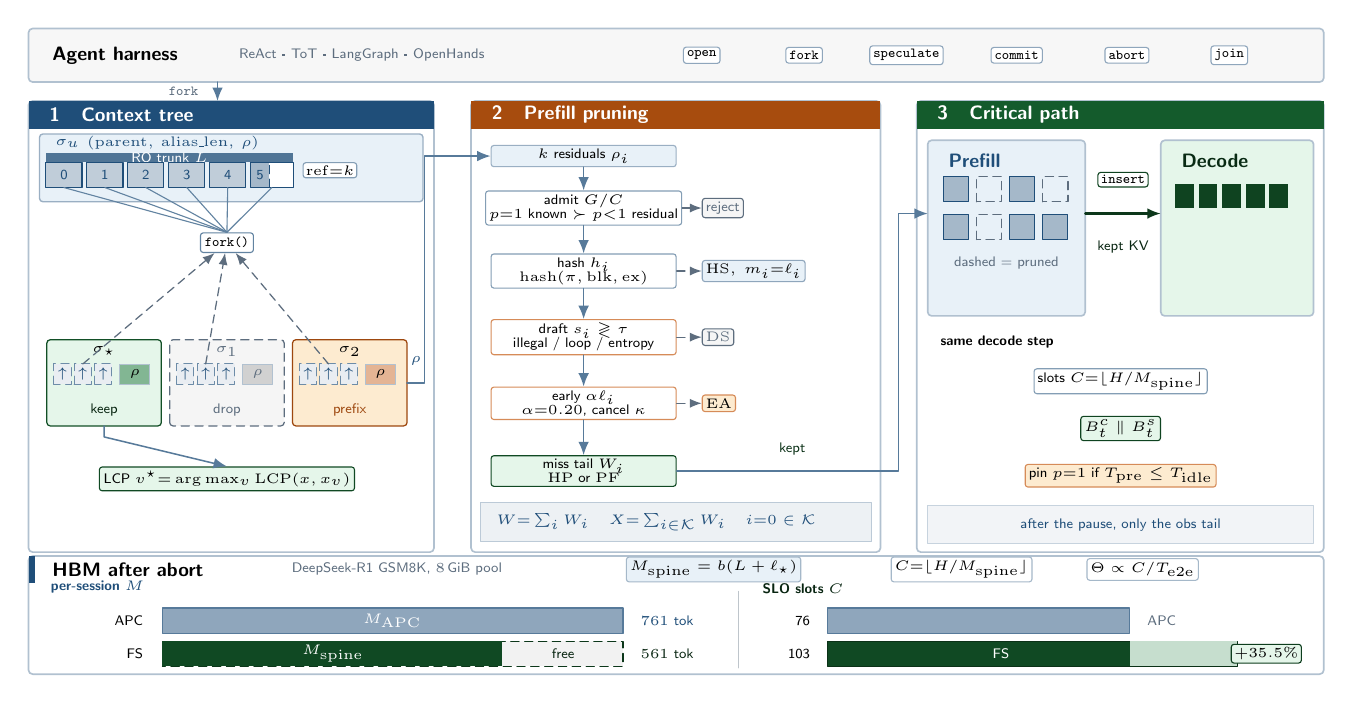
\begin{tikzpicture}[
  x=1cm, y=1cm,
  font=\sffamily,
  >=Latex,
  line cap=round, line join=round,
  panel/.style={draw=fsblue!35, line width=0.6pt, rounded corners=1.5pt, fill=white},
  head/.style={font=\scriptsize\bfseries\sffamily, text=white, anchor=west},
  tinyL/.style={font=\tiny\sffamily, text=fsgray, align=center},
  arr/.style={-{Latex[length=1.7mm,width=1.35mm]}, line width=0.55pt, draw=fsblue!75},
  sarr/.style={-{Latex[length=1.5mm,width=1.15mm]}, line width=0.45pt, draw=fsgray, densely dashed},
  chip/.style={draw, rounded corners=1pt, inner sep=1.3pt, font=\tiny\sffamily, line width=0.4pt},
  leaf/.style={draw, rounded corners=1.2pt, inner sep=1.8pt, align=center,
               font=\tiny\sffamily, line width=0.45pt, minimum width=1.22cm, minimum height=0.64cm},
  forkline/.style={line width=0.85pt, draw=fsblue!80},
]
% ---------- canvas ----------
\path (0,0) rectangle (16.45,8.20);

% ---------- harness ----------
\draw[panel, fill=black!3] (0,7.52) rectangle (16.45,8.20);
\node[font=\scriptsize\bfseries\sffamily, anchor=west] at (0.18,7.86) {Agent harness};
\node[font=\tiny\sffamily, anchor=west, text=fsgray] at (2.55,7.86)
  {ReAct \textperiodcentered\ ToT \textperiodcentered\ LangGraph \textperiodcentered\ OpenHands};
\foreach \x/\t in {8.55/open, 9.85/fork, 11.15/speculate, 12.55/commit, 13.95/abort, 15.25/join} {
  \node[chip, draw=fsblue!50, fill=white] at (\x,7.86) {\texttt{\t}};
}

% ---------- panel frames ----------
\draw[panel] (0,1.55) rectangle (5.15,7.28);
\draw[panel] (5.62,1.55) rectangle (10.82,7.28);
\draw[panel] (11.28,1.55) rectangle (16.45,7.28);
\fill[fsblue] (0,6.92) rectangle (5.15,7.28);
\fill[fsorange!85!black] (5.62,6.92) rectangle (10.82,7.28);
\fill[fsgreen!75!black] (11.28,6.92) rectangle (16.45,7.28);
\node[head] at (0.14,7.10) {1\quad Context tree};
\node[head] at (5.76,7.10) {2\quad Prefill pruning};
\node[head] at (11.42,7.10) {3\quad Critical path};

% ---------- 1. physical frames; k aliases point up; private ρ ----------
\draw[fsblue!45, line width=0.5pt, rounded corners=1.2pt, fill=fslight]
  (0.14,6.00) rectangle (5.01,6.86);
\node[font=\tiny\sffamily\bfseries, text=fsblue, anchor=west] at (0.22,6.74)
  {$\sigma_u$};
\node[font=\tiny\sffamily, text=fsblue, anchor=west] at (0.62,6.74)
  {$(\mathrm{parent},\,\mathrm{alias\_len},\,\rho)$};

\fill[fsblue!78] (0.22,6.50) rectangle (3.36,6.62);
\node[font=\tiny\sffamily, text=white] at (1.79,6.56) {RO trunk $L$};
\foreach \i in {0,...,4} {
  \fill[fsblue!28] ({0.22+\i*0.52},6.18) rectangle ({0.68+\i*0.52},6.50);
  \draw[fsblue, line width=0.4pt] ({0.22+\i*0.52},6.18) rectangle ({0.68+\i*0.52},6.50);
  \node[font=\tiny\sffamily, text=fsblue] at ({0.45+\i*0.52},6.34) {\i};
}
\fill[white] (2.82,6.18) rectangle (3.36,6.50);
\fill[fsblue!40] (2.82,6.18) rectangle (3.06,6.50);
\draw[fsblue, densely dashed, line width=0.4pt] (3.06,6.18) -- (3.06,6.50);
\draw[fsblue, line width=0.4pt] (2.82,6.18) rectangle (3.36,6.50);
\node[font=\tiny\sffamily, text=fsblue] at (2.94,6.34) {5};
\node[chip, draw=fsblue!55, fill=white, inner sep=1.0pt, anchor=west] at (3.48,6.40)
  {$\mathrm{ref}{=}k$};

% fork(): children gather into the call, then it fans out onto each trunk page.
\node[chip, draw=fsblue!70, fill=white, inner sep=1.6pt] (forkfn) at (2.52,5.48)
  {\texttt{fork()}};
\foreach \i in {0,...,4} {
  \draw[fsblue!70, line width=0.4pt] (forkfn.north) -- ({0.45+\i*0.52},6.18);
}
\draw[fsblue!70, line width=0.4pt] (forkfn.north) -- (3.09,6.18);

% children: ↑ slots are PTEs (not copies); ρ is private
\node[inner sep=0, minimum width=1.44cm, minimum height=1.08cm] (bs) at (0.96,3.70) {};
\node[inner sep=0, minimum width=1.44cm, minimum height=1.08cm] (b1) at (2.52,3.70) {};
\node[inner sep=0, minimum width=1.44cm, minimum height=1.08cm] (b2) at (4.08,3.70) {};
\draw[fsgreen!65!black, fill=fscommit, rounded corners=1.2pt, line width=0.45pt]
  (bs.south west) rectangle (bs.north east);
\draw[fsgray, fill=black!4, densely dashed, rounded corners=1.2pt, line width=0.45pt]
  (b1.south west) rectangle (b1.north east);
\draw[fsorange!80!black, fill=fsspec, rounded corners=1.2pt, line width=0.45pt]
  (b2.south west) rectangle (b2.north east);
\node[font=\tiny\sffamily] at (0.96,4.10) {$\sigma_\star$};
\node[font=\tiny\sffamily, text=fsgray] at (2.52,4.10) {$\sigma_1$};
\node[font=\tiny\sffamily] at (4.08,4.10) {$\sigma_2$};
\foreach \x in {0.96,2.52,4.08} {
  \foreach \j in {0,1,2} {
    \fill[fsblue!10] ({\x-0.64+\j*0.26},3.68) rectangle ({\x-0.42+\j*0.26},3.94);
    \draw[fsblue!65, densely dashed, line width=0.35pt]
      ({\x-0.64+\j*0.26},3.68) rectangle ({\x-0.42+\j*0.26},3.94);
    \node[font=\tiny\sffamily, text=fsblue] at ({\x-0.53+\j*0.26},3.81) {$\uparrow$};
  }
  \draw[sarr] ({\x-0.27},3.94) -- (forkfn);
}
\fill[fsgreen!55] (1.16,3.68) rectangle (1.54,3.94);
\fill[black!18] (2.72,3.68) rectangle (3.10,3.94);
\fill[fsorange!45] (4.28,3.68) rectangle (4.66,3.94);
\foreach \x in {1.35,2.91,4.47} {
  \draw[fsblue!35, line width=0.3pt] ({\x-0.19},3.68) rectangle ({\x+0.19},3.94);
}
\node[font=\tiny\sffamily] at (1.35,3.81) {$\rho$};
\node[font=\tiny\sffamily, text=fsgray] at (2.91,3.81) {$\rho$};
\node[font=\tiny\sffamily] at (4.47,3.81) {$\rho$};
\node[font=\tiny\sffamily, text=fsgreen!30!black] at (0.96,3.36) {keep};
\node[font=\tiny\sffamily, text=fsgray] at (2.52,3.36) {drop};
\node[font=\tiny\sffamily, text=fsorange!80!black] at (4.08,3.36) {prefix};

\node[chip, draw=fsgreen!60!black, fill=fscommit, inner sep=1.5pt, align=center] (lcp) at (2.52,2.48)
  {LCP $v^\star{=}\arg\max_v\mathrm{LCP}(x,x_v)$};
\draw[arr] (bs.south) -- ++(0,-0.14) -- (lcp.north);

% ---------- 2. richer APP filter ----------
\node[chip, draw=fsblue!45, fill=fslight, minimum width=2.35cm] (inr) at (7.05,6.58) {$k$ residuals $\rho_i$};
\node[chip, draw=fsblue!55, fill=white, minimum width=2.35cm, align=center] (gc) at (7.05,5.92)
  {admit $G/C$\\[-1pt]{\tiny $p{=}1$ known $\succ$ $p{<}1$ residual}};
\node[chip, draw=fsblue!55, fill=white, minimum width=2.35cm, align=center] (hs) at (7.05,5.12)
  {hash $h_i$\\[-1pt]{\tiny $\mathrm{hash}(\pi,\mathrm{blk},\mathrm{ex})$}};
\node[chip, draw=fsorange!70, fill=white, minimum width=2.35cm, align=center] (dr) at (7.05,4.28)
  {draft $s_i \gtrless \tau$\\[-1pt]{\tiny illegal / loop / entropy}};
\node[chip, draw=fsorange!70, fill=white, minimum width=2.35cm, align=center] (ea) at (7.05,3.44)
  {early $\alpha\ell_i$\\[-1pt]{\tiny $\alpha{=}0.20$, cancel $\kappa$}};
\node[chip, draw=fsgreen!60!black, fill=fscommit, minimum width=2.35cm, align=center] (mt) at (7.05,2.58)
  {miss tail $\Work_i$\\[-1pt]{\tiny $\mathrm{HP}$ or $\mathrm{PF}$}};

\draw[arr] (inr) -- (gc);
\draw[arr] (gc) -- (hs);
\draw[arr] (hs) -- (dr);
\draw[arr] (dr) -- (ea);
\draw[arr] (ea) -- (mt);

\node[chip, draw=fsgray, fill=black!4, text=fsgray, anchor=west, align=left] (sk0) at (8.55,5.92) {reject};
\node[chip, draw=fsblue!50, fill=fslight, anchor=west, align=left] (sk1) at (8.55,5.12) {$\mathrm{HS},\ m_i{=}\ell_i$};
\node[chip, draw=fsgray, fill=black!4, text=fsgray, anchor=west, align=left] (sk2) at (8.55,4.28) {$\mathrm{DS}$};
\node[chip, draw=fsorange!70, fill=fsspec, anchor=west, align=left] (sk3) at (8.55,3.44) {$\mathrm{EA}$};
\draw[sarr] (gc.east) -- (sk0.west);
\draw[sarr] (hs.east) -- (sk1.west);
\draw[sarr] (dr.east) -- (sk2.west);
\draw[sarr] (ea.east) -- (sk3.west);

\fill[fsblue!8] (5.74,1.68) rectangle (10.70,2.18);
\draw[fsblue!30, line width=0.35pt] (5.74,1.68) rectangle (10.70,2.18);
\node[font=\tiny\sffamily, text=fsblue, anchor=west] at (5.82,1.93)
  {$\Work{=}\sum_i \Work_i$ \quad $\Xfer{=}\sum_{i\in\Keep}\Work_i$ \quad $i{=}0\in\Keep$};

% ---------- 3. disaggregated prefill / decode, gated transfer ----------
\draw[panel, rounded corners=1.4pt, fill=fslight] (11.42,4.55) rectangle (13.42,6.78);
\node[font=\scriptsize\bfseries\sffamily, text=fsblue, anchor=west] at (11.56,6.52) {Prefill};
% kept and pruned are interleaved; the last cell stays, so this is not a suffix cut
\foreach \c/\r in {0/1, 2/1, 0/0, 2/0, 3/0} {
  \fill[fsblue!40] ({11.62+\c*0.42},{5.52+\r*0.48}) rectangle ({11.94+\c*0.42},{5.84+\r*0.48});
  \draw[fsblue, line width=0.35pt] ({11.62+\c*0.42},{5.52+\r*0.48}) rectangle ({11.94+\c*0.42},{5.84+\r*0.48});
}
\foreach \c/\r in {1/1, 3/1, 1/0} {
  \draw[fsgray, densely dashed, line width=0.45pt]
    ({11.62+\c*0.42},{5.52+\r*0.48}) rectangle ({11.94+\c*0.42},{5.84+\r*0.48});
}
\node[font=\tiny\sffamily, text=fsgray] at (12.42,5.22) {dashed = pruned};

\draw[panel, rounded corners=1.4pt, fill=fscommit] (14.38,4.55) rectangle (16.32,6.78);
\node[font=\scriptsize\bfseries\sffamily, text=fsgreen!35!black, anchor=west] at (14.52,6.52) {Decode};
\foreach \i in {0,...,4} {
  \fill[fsgreen!55!black] ({14.56+\i*0.30},5.92) rectangle ({14.80+\i*0.30},6.22);
}

\draw[arr, draw=fsgreen!45!black, line width=0.75pt] (13.42,5.85) -- (14.38,5.85);
\node[chip, draw=fsgreen!55!black, fill=white, inner sep=1.1pt] at (13.90,6.28) {\texttt{insert}};
\node[font=\tiny\sffamily, text=fsgreen!30!black] at (13.90,5.42) {kept KV};

% critical path: spine slots, overlap, tool-idle suffix
\node[font=\tiny\sffamily\bfseries, anchor=west] at (11.46,4.22) {same decode step};
\node[chip, draw=fsblue!55, fill=white, align=center] at (13.87,3.72)
  {slots $C{=}\lfloor H/M_{\mathrm{spine}}\rfloor$};
\node[chip, draw=fsgreen!55!black, fill=fscommit, align=center] at (13.87,3.12)
  {$B^c_t \parallel B^s_t$};
\node[chip, draw=fsorange!70, fill=fsspec, align=center] at (13.87,2.52)
  {pin $p{=}1$ if $\Pref\le\Idle$};
\fill[fsblue!6] (11.42,1.66) rectangle (16.32,2.14);
\draw[fsblue!25, line width=0.3pt] (11.42,1.66) rectangle (16.32,2.14);
\node[font=\tiny\sffamily, text=fsblue] at (13.87,1.90)
  {after the pause, only the obs tail};

% residuals into APP; kept miss tail stops at the prefill card edge
\draw[arr] (b2.east) -- ++(0.22,0) |- (5.38,6.58) -- (inr.west);
\node[font=\tiny\sffamily, text=fsblue, anchor=south] at (4.92,3.80) {$\rho$};
\draw[arr] (mt.east) -- (11.05,2.58) -- (11.05,5.85) -- (11.42,5.85);
\node[font=\tiny\sffamily, text=fsgreen!40!black, anchor=south] at (9.70,2.66) {kept};

% ---------- HBM (occupancy vs slots) ----------
\draw[panel] (0,0) rectangle (16.45,1.50);
\fill[fsblue] (0,1.16) rectangle (0.08,1.50);
\node[font=\scriptsize\bfseries\sffamily, anchor=west] at (0.18,1.33) {HBM after abort};
\node[font=\tiny\sffamily, text=fsgray, anchor=west] at (3.22,1.33)
  {DeepSeek-R1 GSM8K, $8$\,GiB pool};
\node[chip, draw=fsblue!40, fill=fslight] at (8.70,1.33) {$M_{\mathrm{spine}}=b(L+\ell_\star)$};
\node[chip, draw=fsblue!40, fill=white] at (11.85,1.33) {$C{=}\lfloor H/M_{\mathrm{spine}}\rfloor$};
\node[chip, draw=fsblue!40, fill=white] at (14.15,1.33) {$\Theta\propto C/T_{\mathrm{e2e}}$};

% occupancy: pool 1.70--7.55 (5.85cm). APC full; FS 0.74 of that.
\node[font=\tiny\sffamily\bfseries, text=fsblue, anchor=south west] at (0.16,0.90) {per-session $M$};
\node[font=\tiny\sffamily, anchor=east] at (1.58,0.68) {APC};
\fill[fsblue!50] (1.70,0.52) rectangle (7.55,0.84);
\draw[fsblue!75, line width=0.4pt] (1.70,0.52) rectangle (7.55,0.84);
\node[font=\tiny\sffamily, text=white] at (4.62,0.68) {$M_{\mathrm{APC}}$};
\node[font=\tiny\sffamily, text=fsblue, anchor=west] at (7.65,0.68) {$761$ tok};

\node[font=\tiny\sffamily, anchor=east] at (1.58,0.26) {FS};
\fill[black!5] (1.70,0.10) rectangle (7.55,0.42);
\draw[fsgreen!45!black, line width=0.4pt, densely dashed] (1.70,0.10) rectangle (7.55,0.42);
\fill[fsgreen!60!black] (1.70,0.10) rectangle ({1.70+0.737*5.85},0.42);
\node[font=\tiny\sffamily, text=white] at ({1.70+0.37*5.85},0.26) {$M_{\mathrm{spine}}$};
\node[font=\tiny\sffamily, text=fsgreen!30!black] at ({1.70+0.87*5.85},0.26) {free};
\node[font=\tiny\sffamily, text=fsgreen!30!black, anchor=west] at (7.65,0.26) {$561$ tok};
\draw[fsgray!40, line width=0.4pt] (9.02,0.08) -- (9.02,1.05);

% slots: max bar 103 → width 5.20cm, origin 10.15
\node[font=\tiny\sffamily\bfseries, text=fsgreen!30!black, anchor=south west] at (9.20,0.90) {SLO slots $C$};
\node[font=\tiny\sffamily, anchor=east] at (10.05,0.68) {76};
\fill[fsblue!50] (10.15,0.52) rectangle ({10.15+76/103*5.20},0.84);
\draw[fsblue!75, line width=0.4pt] (10.15,0.52) rectangle ({10.15+76/103*5.20},0.84);
\node[font=\tiny\sffamily, text=fsgray, anchor=west] at ({10.25+76/103*5.20},0.68) {APC};

\node[font=\tiny\sffamily, anchor=east] at (10.05,0.26) {103};
\fill[fsgreen!60!black] (10.15,0.10) rectangle ({10.15+5.20},0.42);
\draw[fsgreen!40!black, line width=0.4pt] (10.15,0.10) rectangle ({10.15+5.20},0.42);
\fill[fsgreen!25] (10.15+76/103*5.20,0.10) rectangle ({10.15+5.20},0.42);
\node[font=\tiny\sffamily, text=white] at (12.35,0.26) {FS};
\node[chip, draw=fsgreen!50!black, fill=fscommit, inner sep=1.1pt] at (15.72,0.26) {$+35.5\%$};

\draw[arr] (2.4,7.52) -- (2.4,7.28);
\node[font=\tiny\sffamily, text=fsgray, anchor=east] at (2.28,7.40) {\texttt{fork}};
\end{tikzpicture}
\iffalse
% Alternate symbolic drawing. Kept for reuse; not compiled.
% Symbolic architecture. The previous drawing is kept below and is not rendered.
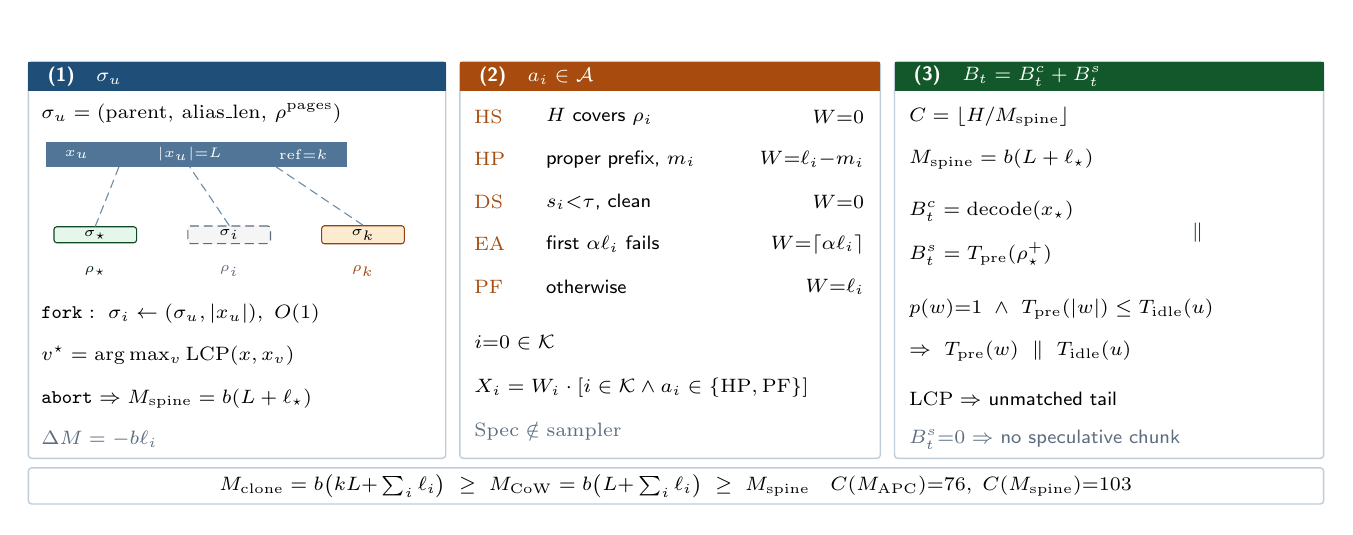
\begin{tikzpicture}[
  x=1cm, y=1cm,
  font=\scriptsize\sffamily,
  >=Latex,
  line cap=round, line join=round,
  panel/.style={draw=fsblue!28, line width=0.5pt, rounded corners=1.2pt, fill=white},
  head/.style={font=\scriptsize\bfseries\sffamily, text=white, anchor=west},
  eq/.style={font=\scriptsize\sffamily, anchor=west, inner sep=0.5pt},
  act/.style={font=\scriptsize\sffamily\bfseries, anchor=west, inner sep=0.4pt},
  alias/.style={densely dashed, line width=0.4pt, draw=fsblue!65},
]
\path (0,0) rectangle (16.45,6.05);

\draw[panel] (0.00,0.58) rectangle (5.30,5.62);
\draw[panel] (5.48,0.58) rectangle (10.82,5.62);
\draw[panel] (11.00,0.58) rectangle (16.45,5.62);
\fill[fsblue] (0.00,5.24) rectangle (5.30,5.62);
\fill[fsorange!85!black] (5.48,5.24) rectangle (10.82,5.62);
\fill[fsgreen!72!black] (11.00,5.24) rectangle (16.45,5.62);
\node[head] at (0.12,5.43) {(1)\quad $\sigma_u$};
\node[head] at (5.60,5.43) {(2)\quad $a_i\in\Act$};
\node[head] at (11.12,5.43) {(3)\quad $B_t=B^c_t+B^s_t$};

% ----- (1) trunk, aliases, private residual -----
\node[eq] at (0.14,4.96)
  {$\sigma_u=(\mathrm{parent},\,\mathrm{alias\_len},\,\rho^{\mathrm{pages}})$};
\fill[fsblue!78] (0.22,4.28) rectangle (4.05,4.60);
\node[font=\tiny\sffamily, text=white, anchor=west] at (0.34,4.44) {$x_u$};
\node[font=\tiny\sffamily, text=white] at (2.05,4.44) {$|x_u|{=}L$};
\node[font=\tiny\sffamily, text=white, anchor=east] at (3.92,4.44) {$\mathrm{ref}{=}k$};

\node[draw=fsgreen!60!black, fill=fscommit, rounded corners=1pt,
      font=\tiny\sffamily, inner sep=1.3pt, minimum width=1.05cm] (s0) at (0.85,3.42) {$\sigma_\star$};
\node[draw=fsgray, fill=black!4, densely dashed, rounded corners=1pt,
      font=\tiny\sffamily, inner sep=1.3pt, minimum width=1.05cm] (si) at (2.55,3.42) {$\sigma_i$};
\node[draw=fsorange!75!black, fill=fsspec, rounded corners=1pt,
      font=\tiny\sffamily, inner sep=1.3pt, minimum width=1.05cm] (sk) at (4.25,3.42) {$\sigma_k$};
\draw[alias] (s0.north) -- (1.15,4.28);
\draw[alias] (si.north) -- (2.05,4.28);
\draw[alias] (sk.north) -- (3.15,4.28);
\node[font=\tiny\sffamily, text=fsgreen!35!black] at (0.85,2.96) {$\rho_\star$};
\node[font=\tiny\sffamily, text=fsgray] at (2.55,2.96) {$\rho_i$};
\node[font=\tiny\sffamily, text=fsorange!80!black] at (4.25,2.96) {$\rho_k$};

\node[eq] at (0.14,2.42) {$\texttt{fork}:\ \sigma_i\leftarrow(\sigma_u,|x_u|),\ O(1)$};
\node[eq] at (0.14,1.88) {$v^\star=\arg\max_v\mathrm{LCP}(x,x_v)$};
\node[eq] at (0.14,1.34) {$\texttt{abort}\Rightarrow M_{\mathrm{spine}}=b(L+\ell_\star)$};
\node[eq, text=fsgray] at (0.14,0.82) {$\Delta M=-b\ell_i$};

% ----- (2) one action per residual -----
\node[act, text=fsorange!85!black] at (5.64,4.92) {$\mathrm{HS}$};
\node[eq] at (6.55,4.92) {$H$ covers $\rho_i$};
\node[eq, anchor=east] at (10.64,4.92) {$\Work{=}0$};

\node[act, text=fsorange!85!black] at (5.64,4.38) {$\mathrm{HP}$};
\node[eq] at (6.55,4.38) {proper prefix, $m_i$};
\node[eq, anchor=east] at (10.64,4.38) {$\Work{=}\ell_i{-}m_i$};

\node[act, text=fsorange!85!black] at (5.64,3.84) {$\mathrm{DS}$};
\node[eq] at (6.55,3.84) {$s_i{<}\tau$, clean};
\node[eq, anchor=east] at (10.64,3.84) {$\Work{=}0$};

\node[act, text=fsorange!85!black] at (5.64,3.30) {$\mathrm{EA}$};
\node[eq] at (6.55,3.30) {first $\alpha\ell_i$ fails};
\node[eq, anchor=east] at (10.64,3.30) {$\Work{=}\lceil\alpha\ell_i\rceil$};

\node[act, text=fsorange!85!black] at (5.64,2.76) {$\mathrm{PF}$};
\node[eq] at (6.55,2.76) {otherwise};
\node[eq, anchor=east] at (10.64,2.76) {$\Work{=}\ell_i$};

\node[eq] at (5.64,2.05) {$i{=}0\in\Keep$};
\node[eq] at (5.64,1.48)
  {$\Xfer_i=\Work_i\cdot[i\in\Keep\wedge a_i\in\{\mathrm{HP},\mathrm{PF}\}]$};
\node[eq, text=fsgray] at (5.64,0.92) {$\mathrm{Spec}\notin\mathrm{sampler}$};

% ----- (3) spine on the critical path -----
\node[eq] at (11.16,4.92) {$C=\lfloor H/M_{\mathrm{spine}}\rfloor$};
\node[eq] at (11.16,4.38) {$M_{\mathrm{spine}}=b(L+\ell_\star)$};
\node[eq] at (11.16,3.72) {$B^c_t=\mathrm{decode}(x_\star)$};
\node[eq] at (11.16,3.18) {$B^s_t=\Pref(\rho^{+}_{\star})$};
\node[font=\scriptsize\sffamily, text=fsgreen!45!black] at (14.85,3.45) {$\parallel$};
\node[eq] at (11.16,2.48) {$p(w){=}1\ \wedge\ \Pref(|w|)\le\Idle(u)$};
\node[eq] at (11.16,1.94) {$\Rightarrow\ \Pref(w)\ \parallel\ \Idle(u)$};
\node[eq] at (11.16,1.34) {$\mathrm{LCP}\Rightarrow$ unmatched tail};
\node[eq, text=fsgray] at (11.16,0.82) {$B^s_t{=}0\Rightarrow$ no speculative chunk};

% ----- occupancy chain -----
\draw[panel] (0,0) rectangle (16.45,0.46);
\node[font=\scriptsize\sffamily] at (8.22,0.23)
  {$M_{\mathrm{clone}}=b\bigl(kL{+}\textstyle\sum_i\ell_i\bigr)
   \;\ge\;
   M_{\mathrm{CoW}}=b\bigl(L{+}\textstyle\sum_i\ell_i\bigr)
   \;\ge\;
   M_{\mathrm{spine}}
   \quad
   C(M_{\mathrm{APC}}){=}76,\; C(M_{\mathrm{spine}}){=}103$};
\end{tikzpicture}

\fi
}
\caption{\textbf{\sys{} architecture.}
(1)~$\sigma_u$ aliases one trunk; \texttt{fork} is $O(1)$; \eqref{eq:lcp} binds the winner.
(2)~One action $a_i$ (\eqref{eq:action}), fixed by the page-aligned match $m_i$.
$m_i=\ell_i$ issues no kernel; $0{<}m_i{<}\ell_i$ prefills the miss; $i{\in}\Lambda$ is withheld; every other miss is prefilled.
$\Xfer$ sums $\Work_i$ over $\Keep$.
(3)~$C=\lfloor H/M_{\mathrm{spine}}\rfloor$.
After abort the live set is the spine, and the same pool admits $76{\to}103$ sessions.}
\label{fig:system}
\end{figure*}

\paragraph{This work.}
\sys is one admission rule on a shared trunk (\Cref{fig:system}, \S\ref{sec:app}).
For residual $\rho_i$, $m_i$ is the longest page-aligned prefix already in the radix index.
That length fixes both the prefill $\Work_i$ and the transfer $\Xfer_i$: a full hit moves nothing, a partial hit moves the miss, a repeated loop ($i{\in}\Lambda$) is withheld, and every other miss is prefilled.
A score below $\tau$ extends past $t_0$ tokens only if the probe meets $\tau$.
Index $0$ stays in $\Keep$, so the connector carries the miss tail of the retained set rather than the $k$-way trunk~\cite{distserve,splitwise}.
The trunk is aliased at \texttt{fork} (\S\ref{sec:state}), which is why $L$ is absent from $\Work_i$ and from $\Xfer_i$; abort leaves $M_{\mathrm{spine}}=b(L+\ell_\star)$.
Decode slots are $C=\lfloor H/M_{\mathrm{spine}}\rfloor$, and any further prefill uses the budget left after committed decode (\S\ref{sec:schedule}).
\eqref{eq:lcp} binds the observed prompt; speculative tokens stay out of the sampler.

\S\ref{sec:eval} measures that rule.
On Qwen3-8B GSM8K, $\tau_{\mathrm{pre}}{=}0.15$ in front of ESC, Speculative Rejection, or DPTS admits $12$ of $16$ residuals, cuts computed prefill by $23\%$ ($5008$ to $3848$), keeps $16/16$ any-finished at $k{=}8$ and $k{=}16$, and reduces ESC time from $17.05$\,s to $14.14$\,s; $\tau_{\mathrm{pre}}{=}0.45$ is faster at $k{=}16$ ($10.93$\,s, still $16/16$) and loses two problems at smaller fan-out (\Cref{tab:prefill-bar,tab:plugin}).
On Qwen3-8B MATH-500, withholding every score below $\tau$ drops any-finished accuracy from $20/32$ to $13/32$ at $k{=}16$; a $128$-token probe restores $20/32$ and cuts end-to-end time from $104.1$\,s to $72.2$\,s (\Cref{tab:grow}).
Across three turns, $48$ of $192$ residuals are prefilled and expand time is $7.9$--$10.6\times$ below APC (\Cref{tab:mt,tab:mt-split}).
The Qwen3-14B spine matches APC accuracy at $0.72\times$ median peak KV, and six model families stay in $0.72$--$0.75\times$ ($n{=}40$).

\section{Background and Model}
\label{sec:problem}

\subsection{Prefill, Decode, and Idle}
Autoregressive inference has two mechanically different phases~\cite{orca,distserve,splitwise}.
\emph{Prefill} consumes the prompt in parallel and is compute-bound; \emph{decode} emits one token (or a small chunk) per step and is memory-bandwidth bound.
PagedAttention~\cite{vllm} stores KV in non-contiguous pages; RadixAttention~\cite{sglang} indexes pages by token prefix so concurrent requests that share a system prompt hit a common trunk.
Two consequences follow for agent workloads.
First, next-turn \ttft{} is the prefill of tokens that miss the cache, plus queuing.
Second, a memory-bound decode batch rarely saturates the tensor cores that a concurrent chunked prefill can use~\cite{sarathi}.
For agents, the prompt of turn $i{+}1$ is a delta on turn $i$, applied after a tool interval of highly variable length~\cite{continuum,mori}.

\subsection{Traditional Methods on a Fan-out}
\label{sec:traditional}
We group under \emph{traditional methods} the mechanisms a production stack already applies to one fan-out: prefix caching, hash-indexed prefill, prefill--decode disaggregation, and decode-time pruning.
Each either shares the trunk or rejects a child, and the stage of that operation is fixed.
\Cref{tab:trad} records the stage.

\begin{table*}[t]
\centering
\caption{Where each traditional method pays for one fan-out of $k$ residuals on a trunk of length $L$.
``First expand'' is the GPU prefill issued before any child has published a block.
``Rejection'' is the earliest point at which a non-winner can leave.
The \sys row is the action of \S\ref{sec:app}.}
\label{tab:trad}
\scriptsize
\setlength{\tabcolsep}{3.5pt}
\begin{tabular}{@{}p{0.20\textwidth}p{0.20\textwidth}p{0.28\textwidth}p{0.24\textwidth}@{}}
\toprule
Method & First expand & Rejection & Connector \\
\midrule
Recompute & $k$ clones of $L$ & end of the request & none \\
APC, radix, hash prefill & $k$ clones of $L$ & LRU after a block is published & none; a later replay of the winner is a hit \\
P/D disaggregation & $k$ clones of $L$ & after \texttt{insert} & $kL+\sum_i\ell_i$ \\
ESC, Speculative Rejection, DPTS & every residual & after a generated prefix & KV of every prefilled child \\
\sys & one alias of $L$ & loop before the kernel; other low scores after a $t_0$ probe & miss tail of $\Keep$ \\
\bottomrule
\end{tabular}
\end{table*}

\paragraph{First-expand cost.}
APC indexes a full block by $h=\mathrm{hash}(\mathrm{parent},\;\mathrm{tokens},\;\mathrm{extra})$ after those tokens exist~\cite{vllm}; RadixAttention indexes the same prefix~\cite{sglang}.
A same-batch expansion therefore misses and clones $k$ trunks,
$\Work_{\mathrm{APC}}=kL+\sum_i\ell_i$,
while a later replay of $x_\star$ is a hit ($\Work{=}0$).
Baseline disaggregation~\cite{distserve,splitwise} transfers that span,
\begin{equation}
\label{eq:xfer-stock}
\Xfer_{\mathrm{PD}}=kL+\textstyle\sum_i\ell_i,
\end{equation}
so $\Xfer_{\mathrm{PD}}=\Work_{\mathrm{APC}}$ on the first expand.
ESC~\cite{esc}, Speculative Rejection~\cite{specrej}, and DPTS~\cite{dpts} evaluate a child only after its prefill and a generated prefix, hence after $\Work$ and, under disaggregation, after $\Xfer$.

\subsection{Fan-out Model}
\label{sec:model}

\begin{definition}[Branching step]
\label{def:step}
A parent $u$ holds a committed trunk $x_u$ with $|x_u|{=}L$.
A fan-out is a set of residuals $\{\rho_i\}_{i=1}^{k}$, $|\rho_i|{=}\ell_i$.
The bound winner $\star$ leaves the spine $x_\star=x_u\Vert\rho_\star$, $|x_\star|{=}L{+}\ell_\star$.
\end{definition}

Let $b$ be KV bytes per token and $P$ the page size.
The three occupancies of one step are
\begin{align}
M_{\mathrm{clone}} &= b\bigl(kL+\textstyle\sum_i\ell_i\bigr), \label{eq:mem}\\
M_{\mathrm{CoW}} &= b\bigl(L+\textstyle\sum_i\ell_i\bigr), \nonumber\\
M_{\mathrm{spine}} &= b\bigl(L+\ell_\star\bigr). \nonumber
\end{align}
$M_{\mathrm{clone}}$ is the first-expand footprint of recompute, APC, and baseline disaggregation;
$M_{\mathrm{CoW}}$ is one shared trunk with every residual live;
$M_{\mathrm{spine}}$ is the footprint after abort.
$\Work$ is the token count issued to a prefill kernel before $\star$ is known;
$\Xfer$ is the token count inserted on the P/D connector.
\Cref{tab:notation} lists the remaining symbols.

\begin{table}[t]
\centering
\caption{Notation for Definition~\ref{def:step} and for \eqref{eq:action}--\eqref{eq:xfer}.}
\label{tab:notation}
\scriptsize
\setlength{\tabcolsep}{3.2pt}
\begin{tabular}{@{}llp{0.58\columnwidth}@{}}
\toprule
Symbol & Domain & Meaning \\
\midrule
$L$, $\ell_i$, $\ell_\star$ & $\mathbb{N}$ & trunk; residual $i$; committed residual \\
$\rho_i$, $x_u$ & tokens & residual of child $i$; committed trunk \\
$h_i$ & digest & $\mathrm{hash}(\mathrm{parent},\rho_i[0{:}P),\mathrm{extra})$ \\
$m_i$ & tokens & full-page prefix of $\rho_i$ in $H$, steps of $P$ \\
$s_i$, $s'_i$, $\tau$ & $[0,1]$ & score of $\rho_i$; score of the probe $y_i$; threshold \\
$t_0$, $D$, $d_i$ & tokens & probe length; decode budget; length assigned to $i$ \\
$\alpha$ & $(0,1]$ & early-abort prefix fraction ($0.20$) \\
$p_i$, $q_i$ & $[0,1]$ & admit probability; residual-prefix hit rate \\
$a_i\in\Act$ & $\Act$ & $\mathrm{HS},\mathrm{HP},\mathrm{DS},\mathrm{EA},\mathrm{PF}$ (\eqref{eq:action}) \\
$\Lambda$, $F_i$ & set, $\{0,1\}$ & repeated-loop index set; early-abort predicate \\
$\Keep$ & $\subseteq[k]$ & residuals that remain after admission \\
$\Work_i$, $\Xfer_i$ & tokens & GPU miss tail; connector payload \\
$b$, $P$ & bytes, tok & KV bytes per token; page size \\
$B_t=B^c_t+B^s_t$ & tokens & committed and speculative budget on tick $t$ \\
\bottomrule
\end{tabular}
\end{table}

\section{Design}
\label{sec:design}

\sys lies between the agent runtime and the LLM engine (\Cref{fig:system}).
The harness exposes branch structure; the control plane admits, prunes, binds, and retains; the backend moves pages and tokens.

\subsection{API}
\label{sec:overview}
\begin{center}
\footnotesize
\setlength{\tabcolsep}{3pt}
\begin{tabular}{@{}lp{0.56\columnwidth}@{}}
\toprule
\texttt{open(session)} & Create a root; prefill system+user. \\
\texttt{fork(u, bid, tok?)} & Child of $u$; optional known suffix. \\
\texttt{speculate(v, pri)} & Mark $v$ eligible for speculative prefill. \\
\texttt{commit(u, tokens)} & Bind by LCP; start decode. \\
\texttt{join(children, pol)} & Merge fan-out (\texttt{all}/\texttt{first}/\texttt{kofn}). \\
\texttt{abort(v)} / \texttt{close} & Drop a subtree; end the session. \\
\bottomrule
\end{tabular}
\end{center}
\texttt{commit} is the only operator on the critical path of user-visible tokens.

\subsection{Copy-on-Write Context Tree}
\label{sec:state}

\begin{definition}[Context tree]
A session is a rooted tree $T=(V,E)$.
Node $u$ stores a token sequence $x_u$ such that $x_{\pi(u)}\preceq x_u$, a residual $\delta_u=x_u[|x_{\pi(u)}|{:}]$, a mode $\rho_u\in\{\textsc{Spec},\textsc{Commit},\textsc{Idle},\textsc{Dead}\}$, a generation $g_u$, and a logical page table
$\sigma_u=(\mathrm{parent},\;\mathrm{alias\_len},\;\rho^{\mathrm{pages}}_u)$.
\end{definition}

Invariants: (i)~prefix; (ii)~at most one committed child per node except during join; (iii)~speculative nodes are invisible to sampling; (iv)~a page's refcount equals the number of non-dead nodes that map it.
\texttt{fork}$(u,\mathit{bid},x^{\mathrm{k}})$ copies two words $(\mathrm{parent}\leftarrow\sigma_u,\;\mathrm{alias\_len}\leftarrow|x_u|)$ and increfs the aliased frames---$O(1)$ in $L$.
A write that hits $\mathrm{ref}>1$ or a read-only tail CoW-copies only the valid rows.
\Cref{fig:pool} is that pool.
A multi-level fan-out is a \emph{sequence} of CoWs (\Cref{fig:tree}): each edge aliases the parent and allocates only $+$r; live paths share every page on the common prefix; abort is residual-only, and a subtree with no live child cascades until the committed spine.
The two compose: LCP commit publishes full winner pages into the APC index so a later session can hash-hit them (\S\ref{sec:app}).
Abort frees $b\ell_i$ bytes, not $b(L+\ell_i)$.
TTL and offload are node-granular: speculative leaves first, then idle committed leaves, then the spine~\cite{continuum,mori}.

\begin{figure*}[t]
\centering
\resizebox{\textwidth}{!}{% Context-tree page pool. Logical verbs left, physical frames right.
\tikzset{
  fmbadge/.style={circle,draw=#1!70!black,fill=#1,text=white,
    font=\tiny\sffamily\bfseries,inner sep=0pt,minimum size=0.32cm},
  fmcard/.style={draw=#1!65,fill=#1!8,rounded corners=1.6pt,align=center,
    inner sep=2pt,font=\tiny\sffamily,line width=0.45pt},
  pg/.style 2 args={draw=#1,fill=#2,rounded corners=1.3pt,align=center,
    font=\tiny\sffamily,inner sep=1pt,minimum width=1.05cm,
    minimum height=0.70cm,line width=0.4pt},
  fp/.style={draw=fsgray,fill=black!5,rounded corners=1.2pt,align=center,
    font=\tiny\sffamily,inner sep=1pt,minimum width=0.72cm,
    minimum height=0.38cm,line width=0.35pt,text=black!70},
  note/.style={font=\tiny\sffamily,text=black!58},
  hdr/.style={font=\scriptsize\sffamily\bfseries},
  fmdata/.style={-{Latex[length=1.4mm]},line width=0.5pt,draw=fsblue!75},
  fmfeed/.style={densely dashed,-{Latex[length=1.4mm]},line width=0.5pt},
  flink/.style={{Latex[length=1.1mm,width=0.8mm]}-{Latex[length=1.1mm,width=0.8mm]},
    line width=0.36pt,draw=fsgray},
  tbox/.style={draw=#1!70!black,fill=#1!10,rounded corners=1.2pt,align=center,
    font=\tiny\sffamily,inner sep=1.2pt,line width=0.4pt},
}
\begin{tikzpicture}[x=1cm,y=1cm,font=\sffamily,
  >=Latex,line cap=round,line join=round]
\path (-0.02,-0.32) rectangle (14.72,5.78);
% ========================== zones ==========================
\fill[black!3.5,rounded corners=5pt] (0.04,0.08) rectangle (6.08,5.52);
\fill[fsblue!5,rounded corners=5pt] (6.24,0.08) rectangle (14.58,5.52);
\draw[black!22,dashed,dash pattern=on 1.2pt off 1.4pt,line width=0.5pt]
  (6.16,0.18) -- (6.16,5.38);
\node[anchor=west,hdr,text=fsgray] at (0.16,5.38) {LOGICAL \(\cdot\) TREE VERBS};
\node[anchor=west,hdr,text=fsblue] at (6.40,5.38) {PHYSICAL \(\cdot\) FRAME POOL};
% ===================== 1. request table =====================
\fill[white,rounded corners=2.5pt] (0.18,4.18) rectangle (5.92,5.28);
\fill[fsblue!16,rounded corners=2.5pt] (0.18,4.96) rectangle (5.92,5.28);
\fill[fsblue!16] (0.18,4.96) rectangle (5.92,5.08);
\draw[fsblue!65,rounded corners=2.5pt,line width=0.5pt] (0.18,4.18) rectangle (5.92,5.28);
\node[fmbadge=fsblue] at (0.42,5.12) {1};
\node[anchor=west,font=\tiny\sffamily\bfseries] at (0.64,5.12) {Request table \(\sigma_u\)};
\node[tbox=fsblue,minimum width=0.64cm,minimum height=0.30cm] (uu) at (1.22,4.74) {\(u\)};
\node[tbox=fsorange,minimum width=0.70cm,minimum height=0.30cm] (v1) at (0.52,4.40) {\(\sigma_1\)};
\node[tbox=fsgreen,minimum width=0.70cm,minimum height=0.30cm] (vs) at (1.36,4.40) {\(\sigma_\star\)};
\node[tbox=fsgray,minimum width=0.56cm,minimum height=0.30cm] (vk) at (2.12,4.40) {\(\cdots\)};
\draw[fsblue!70,densely dashed,line width=0.45pt] (uu.south) -- (v1.north);
\draw[fsblue!70,densely dashed,line width=0.45pt] (uu.south) -- (vs.north);
\draw[fsblue!70,densely dashed,line width=0.45pt] (uu.south) -- (vk.north);
\node[fmcard=fsblue,anchor=west,align=left,text width=2.85cm,minimum height=0.62cm]
  at (2.62,4.56)
  {\(\sigma_u{=}(\mathrm{parent},\,\mathrm{alias\_len},\,\rho)\)\\[1pt]
   \(\mathrm{ref}(p){=}\#\) live mappers};
% ===================== 2. fork =====================
\fill[white,rounded corners=2.5pt] (0.18,3.02) rectangle (5.92,4.04);
\fill[fsblue!16,rounded corners=2.5pt] (0.18,3.72) rectangle (5.92,4.04);
\fill[fsblue!16] (0.18,3.72) rectangle (5.92,3.84);
\draw[fsblue!65,rounded corners=2.5pt,line width=0.5pt] (0.18,3.02) rectangle (5.92,4.04);
\node[fmbadge=fsblue] at (0.42,3.88) {2};
\node[anchor=west,font=\tiny\sffamily\bfseries] at (0.64,3.88)
  {\texttt{fork}\((u)\): two words, \(O(1)\) in \(L\)};
\node[fmcard=fsblue,minimum width=1.55cm,minimum height=0.40cm] (cp) at (1.15,3.42)
  {\(\mathrm{parent}\leftarrow\sigma_u\)};
\node[fmcard=fsblue,minimum width=1.62cm,minimum height=0.40cm] (ca) at (2.95,3.42)
  {\(\mathrm{alias\_len}\leftarrow|x_u|\)};
\node[fmcard=fsorange,minimum width=1.35cm,minimum height=0.40cm] (ci) at (4.85,3.42)
  {incref trunk};
\draw[fmdata] (cp) -- (ca);
\draw[fmdata] (ca) -- (ci);
\node[note] at (3.05,3.16) {no memcpy of \(L\)};
% ===================== 6. LCP =====================
\fill[white,rounded corners=2.5pt] (0.18,1.52) rectangle (5.92,2.88);
\fill[fsgreen!18,rounded corners=2.5pt] (0.18,2.56) rectangle (5.92,2.88);
\fill[fsgreen!18] (0.18,2.56) rectangle (5.92,2.68);
\draw[fsgreen!60!black,rounded corners=2.5pt,line width=0.5pt] (0.18,1.52) rectangle (5.92,2.88);
\node[fmbadge=fsgreen] at (0.42,2.72) {6};
\node[anchor=west,font=\tiny\sffamily\bfseries] at (0.64,2.72) {LCP commit};
\node[fmcard=fsgreen,minimum width=5.35cm,minimum height=0.34cm] at (3.05,2.36)
  {\(v^\star{=}\arg\max_v\mathrm{LCP}(x,x_v)\)};
\node[fmcard=fsgreen,minimum width=5.35cm,minimum height=0.34cm] at (3.05,1.98)
  {\(H\leftarrow H\cup\{x_\star\}\)};
\node[fmcard=fspurple,minimum width=5.35cm,minimum height=0.34cm] at (3.05,1.66)
  {\(g\leftarrow g{+}1\) retires in-flight spec};
% ===================== 7. abort =====================
\fill[white,rounded corners=2.5pt] (0.18,0.16) rectangle (5.92,1.38);
\fill[fsorange!18,rounded corners=2.5pt] (0.18,1.06) rectangle (5.92,1.38);
\fill[fsorange!18] (0.18,1.06) rectangle (5.92,1.18);
\draw[fsorange!70,rounded corners=2.5pt,line width=0.5pt] (0.18,0.16) rectangle (5.92,1.38);
\node[fmbadge=fsorange] at (0.42,1.22) {7};
\node[anchor=west,font=\tiny\sffamily\bfseries] at (0.64,1.22) {\texttt{abort}};
\node[fmcard=fsorange,minimum width=5.35cm,minimum height=0.46cm] at (3.05,0.62)
  {\(M_{\mathrm{spine}}{=}b(L{+}\ell_\star)\)\\[1pt] free \(b\ell_i\), not \(b(L{+}\ell_i)\)};
% ===================== 3. frames =====================
\fill[fsblue!7,rounded corners=3pt] (6.38,3.02) rectangle (14.44,5.28);
\draw[fsblue!45,rounded corners=3pt,line width=0.5pt] (6.38,3.02) rectangle (14.44,5.28);
\node[fmbadge=fsblue] at (6.60,5.08) {3};
\node[anchor=west,font=\tiny\sffamily] at (6.82,5.08) {\textbf{Shared trunk, private \(\rho\)}};
\node[pg={fsblue}{fslight},minimum width=2.35cm,minimum height=0.92cm] at (7.75,4.22)
  {\textbf{shared trunk}\\[-1pt] one copy of \(L\)\\[-1pt] read-only};
\node[pg={fsorange!80!black}{fsspec},minimum width=2.35cm,minimum height=0.92cm] at (10.35,4.22)
  {\textbf{private \(\rho\)}\\[-1pt] new frames only\\[-1pt] \(\mathrm{ref}{=}1\), not in \(H\)};
\node[pg={fsorange!80!black}{fsspec},densely dashed,minimum width=2.35cm,minimum height=0.92cm] at (12.95,4.22)
  {\textbf{partial tail}\\[-1pt] last page \(n{<}P\)\\[-1pt] not published};
\node[note] at (10.41,3.42)
  {child aliases \(L\);\ a write with \(\mathrm{ref}{>}1\) copies that page's valid rows};
% ===================== 4. hash index =====================
\fill[fsgreen!8,rounded corners=3pt] (6.38,1.52) rectangle (14.44,2.88);
\draw[fsgreen!50!black,rounded corners=3pt,line width=0.5pt] (6.38,1.52) rectangle (14.44,2.88);
\node[fmbadge=fsgreen] at (6.60,2.68) {4};
\node[anchor=west,font=\tiny\sffamily] at (6.82,2.68) {\textbf{Publish index \(H\)}};
\node[fmcard=fsgreen,minimum width=3.55cm,minimum height=0.62cm] at (8.40,2.02)
  {in \(H\): full committed block\\[-1pt] \(h(\mathrm{parent},\mathrm{block})\)};
\node[fmcard=fsorange,minimum width=3.55cm,minimum height=0.62cm] at (12.35,2.02)
  {out of \(H\): speculative\\[-1pt] or partial page};
% ===================== 5. free list =====================
\fill[black!3,rounded corners=3pt] (6.38,0.16) rectangle (14.44,1.38);
\draw[fsgray!70,rounded corners=3pt,line width=0.5pt] (6.38,0.16) rectangle (14.44,1.38);
\node[fmbadge=fsgray] at (6.60,1.18) {5};
\node[anchor=west,font=\tiny\sffamily] at (6.82,1.18) {\textbf{Free list}\quad \(\mathrm{ref}{=}0\)};
\node[fmcard=fsblue,minimum width=3.55cm,minimum height=0.58cm] at (8.40,0.58)
  {\texttt{fork} takes free frames\\[-1pt] for the new \(\rho\)};
\node[fmcard=fsorange,minimum width=3.55cm,minimum height=0.58cm] at (12.35,0.58)
  {\texttt{abort} returns those frames\\[-1pt] trunk stays allocated};
% ===================== cross-boundary =====================
\draw[fmfeed,draw=fsblue,rounded corners=1.5pt]
  (5.92,3.42) -- (6.28,3.42) -- (6.28,4.28) -- (6.55,4.28);
\draw[fmfeed,draw=fsgreen!50!black] (5.92,1.98) -- (6.55,1.98);
\draw[fmfeed,draw=fsorange!80!black] (5.92,0.62) -- (6.55,0.62);
% ===================== legend =====================
\node[anchor=west,font=\tiny\sffamily,text=black!58] at (0.06,-0.14)
  {\textcolor{fsblue}{trunk}\,\(\cdot\)\,%
   \textcolor{fsorange}{residual}\,\(\cdot\)\,%
   \textcolor{fsgreen}{publish}\,\(\cdot\)\,%
   \textcolor{fspurple}{generation}\,\(\cdot\)\,%
   \textcolor{fsgray}{free}\qquad
   dashed edge \(=\) alias};
\end{tikzpicture}
\iffalse
% Alternate symbolic drawing. Kept for reuse; not compiled.
% Symbolic page pool. The previous drawing is kept below and is not rendered.
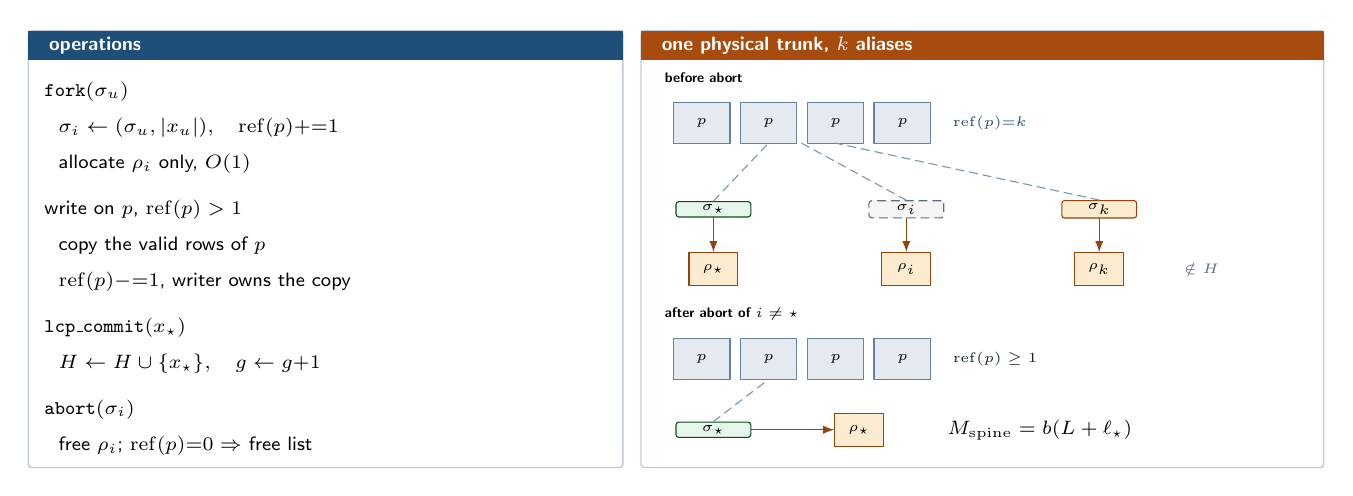
\begin{tikzpicture}[
  x=1cm, y=1cm,
  font=\scriptsize\sffamily,
  >=Latex,
  line cap=round, line join=round,
  panel/.style={draw=fsblue!28, line width=0.5pt, rounded corners=1.2pt, fill=white},
  head/.style={font=\scriptsize\bfseries\sffamily, text=white, anchor=west},
  eq/.style={font=\scriptsize\sffamily, anchor=west, inner sep=0.5pt},
  pg/.style={draw=fsblue!70, fill=fsblue!12, minimum width=0.72cm, minimum height=0.52cm,
             font=\tiny\sffamily, inner sep=1pt},
  priv/.style={draw=fsorange!75!black, fill=fsspec, minimum width=0.62cm, minimum height=0.42cm,
               font=\tiny\sffamily, inner sep=0.6pt},
  alias/.style={densely dashed, line width=0.4pt, draw=fsblue!60},
]
\path (0,0) rectangle (16.45,5.55);

\draw[panel] (0,0) rectangle (7.55,5.55);
\draw[panel] (7.78,0) rectangle (16.45,5.55);
\fill[fsblue] (0,5.18) rectangle (7.55,5.55);
\fill[fsorange!85!black] (7.78,5.18) rectangle (16.45,5.55);
\node[head] at (0.14,5.36) {operations};
\node[head] at (7.92,5.36) {one physical trunk, $k$ aliases};

\node[eq] at (0.18,4.78) {$\texttt{fork}(\sigma_u)$};
\node[eq] at (0.36,4.32) {$\sigma_i\leftarrow(\sigma_u,|x_u|),\quad \mathrm{ref}(p){+}{=}1$};
\node[eq] at (0.36,3.86) {allocate $\rho_i$ only,\ $O(1)$};

\node[eq] at (0.18,3.28) {write on $p$,\ $\mathrm{ref}(p)>1$};
\node[eq] at (0.36,2.82) {copy the valid rows of $p$};
\node[eq] at (0.36,2.36) {$\mathrm{ref}(p){-}{=}1$, writer owns the copy};

\node[eq] at (0.18,1.78) {$\texttt{lcp\_commit}(x_\star)$};
\node[eq] at (0.36,1.32) {$H\leftarrow H\cup\{x_\star\},\quad g\leftarrow g{+}1$};

\node[eq] at (0.18,0.74) {$\texttt{abort}(\sigma_i)$};
\node[eq] at (0.36,0.28) {free $\rho_i$;\ $\mathrm{ref}(p){=}0\Rightarrow$ free list};

% right: before abort — shared pages, private residual
\node[font=\tiny\sffamily\bfseries, anchor=west] at (7.96,4.95) {before abort};
\foreach \x in {8.55,9.40,10.25,11.10} {
  \node[pg] at (\x,4.38) {$p$};
}
\node[font=\tiny\sffamily, anchor=west, text=fsblue] at (11.62,4.38) {$\mathrm{ref}(p){=}k$};
\node[draw=fsgreen!60!black, fill=fscommit, rounded corners=1pt, font=\tiny\sffamily,
      inner sep=1.2pt, minimum width=0.95cm] (a0) at (8.70,3.28) {$\sigma_\star$};
\node[draw=fsgray, fill=black!4, densely dashed, rounded corners=1pt, font=\tiny\sffamily,
      inner sep=1.2pt, minimum width=0.95cm] (a1) at (11.15,3.28) {$\sigma_i$};
\node[draw=fsorange!75!black, fill=fsspec, rounded corners=1pt, font=\tiny\sffamily,
      inner sep=1.2pt, minimum width=0.95cm] (ak) at (13.60,3.28) {$\sigma_k$};
\draw[alias] (a0.north) -- (9.40,4.12);
\draw[alias] (a1.north) -- (9.82,4.12);
\draw[alias] (ak.north) -- (10.25,4.12);
\node[priv] (r0) at (8.70,2.52) {$\rho_\star$};
\node[priv] (r1) at (11.15,2.52) {$\rho_i$};
\node[priv] (rk) at (13.60,2.52) {$\rho_k$};
\draw[-{Latex[length=1.4mm]}, line width=0.4pt, draw=fsorange!75!black] (a0.south) -- (r0.north);
\draw[-{Latex[length=1.4mm]}, line width=0.4pt, draw=fsorange!75!black] (a1.south) -- (r1.north);
\draw[-{Latex[length=1.4mm]}, line width=0.4pt, draw=fsorange!75!black] (ak.south) -- (rk.north);
\node[font=\tiny\sffamily, text=fsgray, anchor=west] at (14.55,2.52) {$\notin H$};

% right: after
\node[font=\tiny\sffamily\bfseries, anchor=west] at (7.96,1.95) {after abort of $i\neq\star$};
\foreach \x in {8.55,9.40,10.25,11.10} {
  \node[pg] at (\x,1.38) {$p$};
}
\node[font=\tiny\sffamily, anchor=west, text=fsgreen!35!black] at (11.62,1.38) {$\mathrm{ref}(p)\ge 1$};
\node[draw=fsgreen!60!black, fill=fscommit, rounded corners=1pt, font=\tiny\sffamily,
      inner sep=1.2pt, minimum width=0.95cm] (b0) at (8.70,0.48) {$\sigma_\star$};
\draw[alias] (b0.north) -- (9.40,1.12);
\node[priv] (rb) at (10.55,0.48) {$\rho_\star$};
\draw[-{Latex[length=1.4mm]}, line width=0.4pt, draw=fsorange!75!black] (b0.east) -- (rb.west);
\node[font=\scriptsize\sffamily, anchor=west] at (11.55,0.48)
  {$M_{\mathrm{spine}}=b(L+\ell_\star)$};
\end{tikzpicture}

\fi
}
\caption{\textbf{Context-tree page pool.}
\texttt{fork} aliases the trunk in $O(1)$ and allocates only $\rho$~\textcircled{1}--\textcircled{3}.
LCP commit publishes $x_\star$ into $H$~\textcircled{4}\textcircled{6}.
\texttt{abort} returns residual frames only, so live occupancy is the spine $M_{\mathrm{spine}}{=}b(L{+}\ell_\star)$~\textcircled{5}\textcircled{7}.}
\label{fig:pool}
\end{figure*}

\subsection{Admission and Commit}
\label{sec:speculate}
A candidate of parent $u$ is a pair $(x^{\mathrm{k}},\hat{x}^{\mathrm{o}})$ with admit probability $p$ and prefix-hit rate $q$.
Known suffixes ($p{=}q{=}1$) precede observation residuals ($q{<}1$), subject to $\Idle(u)$, residual HBM, and branch cap $m$.
Admission stores a future prompt prefix rather than draft output tokens~\cite{speculative,medusa}.

\paragraph{LCP commit.}
On prompt $x$ at $u$,
\begin{equation}
\label{eq:lcp}
v^\star=\arg\max_{v}\mathrm{LCP}(x,x_v),\qquad
g_u\leftarrow g_u+1.
\end{equation}
Pages of the LCP become committed; the unmatched tail is a committed prefill; every sibling aborts.
A job tagged $g\neq g_u$ drops in $O(1)$.
Committed decode attends only $\mathrm{KV}(x_{v^\star})$, so the emitted tokens match a baseline that prefills committed tokens only.

\subsection{Admission Rule}
\label{sec:app}

One action $a_i$ fixes the pair $(\Work_i,\Xfer_i)$ for residual $\rho_i$ (\Cref{fig:app}).
$a_i$ reads $m_i$ first, because a radix match costs no model FLOPs.
On a miss it reads $i{\in}\Lambda$, because a repeated loop is known before a kernel.
Only a miss outside $\Lambda$ enters the kernel, and $F_i$ stops that kernel at $\lceil\alpha\ell_i\rceil$.
$\Xfer_i$ equals $\Work_i$ on $\Keep$ and is zero otherwise, so the connector moves the unmatched suffix of retained residuals.
Index $0$ is in $\Keep$; pages stay out of $H$ until \eqref{eq:lcp}.
The alias of \S\ref{sec:state} is what removes $L$ from both quantities.
On Qwen3-14B GSM8K the alias already stores less KV than APC, while median fan-out is $140$\,ms against $87$\,ms because every residual is still prefilled; $a_i$ is the term that removes that prefill.

\begin{figure*}[t]
\centering
\resizebox{\textwidth}{!}{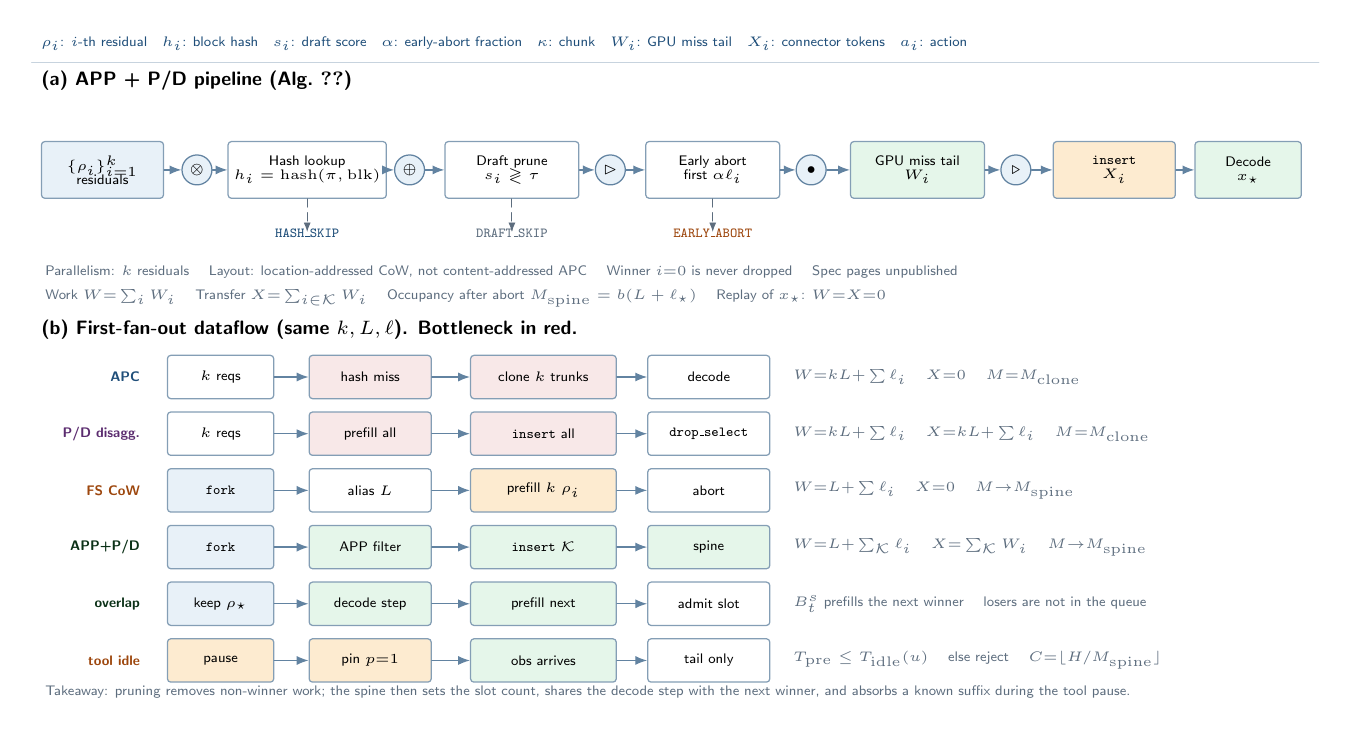
\begin{tikzpicture}[
  x=1cm, y=1cm,
  font=\sffamily,
  >=Latex,
  line cap=round, line join=round,
  box/.style={draw=fsblue!55, rounded corners=1.2pt, fill=white, inner sep=2.2pt,
              align=center, font=\tiny\sffamily, line width=0.45pt, minimum height=0.72cm},
  op/.style={circle, draw=fsblue!70, fill=fslight, inner sep=0.4pt,
             font=\tiny\sffamily\bfseries, minimum size=0.38cm, line width=0.45pt},
  lab/.style={font=\tiny\sffamily, text=fsgray, align=center},
  arr/.style={-{Latex[length=1.5mm,width=1.15mm]}, line width=0.45pt, draw=fsblue!70},
  sarr/.style={-{Latex[length=1.2mm,width=0.9mm]}, densely dashed, draw=fsgray, line width=0.35pt},
]
\path (0,-1.50) rectangle (16.50,7.15);

% ===== legend =====
\node[font=\tiny\sffamily, anchor=west, text=fsblue] at (0.05,6.95)
  {$\rho_i$: $i$-th residual\quad
   $h_i$: block hash\quad
   $s_i$: draft score\quad
   $\alpha$: early-abort fraction\quad
   $\kappa$: chunk\quad
   $\Work_i$: GPU miss tail\quad
   $\Xfer_i$: connector tokens\quad
   $a_i$: action};
\draw[fsblue!25, line width=0.3pt] (0.05,6.72) -- (16.40,6.72);

% ===== (a) APP+PD pipeline =====
\node[font=\scriptsize\bfseries\sffamily, anchor=west] at (0.05,6.48)
  {(a) \app{} + P/D pipeline (Alg.~\ref{alg:app})};

\node[box, fill=fslight, minimum width=1.55cm] (r) at (0.95,5.35)
  {$\{\rho_i\}_{i=1}^{k}$\\[-1pt]{\tiny residuals}};
\node[op] (o1) at (2.15,5.35) {$\otimes$};
\node[box, minimum width=1.85cm] (h) at (3.55,5.35)
  {Hash lookup\\[-1pt]{\tiny $h_i=\mathrm{hash}(\pi,\mathrm{blk})$}};
\node[op] (o2) at (4.85,5.35) {$\oplus$};
\node[box, minimum width=1.70cm] (d) at (6.15,5.35)
  {Draft prune\\[-1pt]{\tiny $s_i\gtrless\tau$}};
\node[op] (o3) at (7.40,5.35) {$\rhd$};
\node[box, minimum width=1.70cm] (e) at (8.70,5.35)
  {Early abort\\[-1pt]{\tiny first $\alpha\ell_i$}};
\node[op] (o4) at (9.95,5.35) {$\bullet$};
\node[box, fill=fscommit, minimum width=1.70cm] (g) at (11.30,5.35)
  {GPU miss tail\\[-1pt]{\tiny $\Work_i$}};
\node[op] (o5) at (12.55,5.35) {$\triangleright$};
\node[box, fill=fsspec, minimum width=1.55cm] (x) at (13.80,5.35)
  {\texttt{insert}\\[-1pt]{\tiny $\Xfer_i$}};
\node[box, fill=fscommit, minimum width=1.35cm] (dec) at (15.50,5.35)
  {Decode\\[-1pt]{\tiny $x_\star$}};

\draw[arr] (r) -- (o1);
\draw[arr] (o1) -- (h);
\draw[arr] (h) -- (o2);
\draw[arr] (o2) -- (d);
\draw[arr] (d) -- (o3);
\draw[arr] (o3) -- (e);
\draw[arr] (e) -- (o4);
\draw[arr] (o4) -- (g);
\draw[arr] (g) -- (o5);
\draw[arr] (o5) -- (x);
\draw[arr] (x) -- (dec);

% side exits
\node[lab, text=fsblue] at (3.55,4.55) {\texttt{HASH\_SKIP}};
\node[lab] at (6.15,4.55) {\texttt{DRAFT\_SKIP}};
\node[lab, text=fsorange!80!black] at (8.70,4.55) {\texttt{EARLY\_ABORT}};
\draw[sarr] (h.south) -- ++(0,-0.42);
\draw[sarr] (d.south) -- ++(0,-0.42);
\draw[sarr] (e.south) -- ++(0,-0.42);

% annotations under (a)
\node[lab, anchor=west] at (0.10,4.05)
  {Parallelism: $k$ residuals \quad
   Layout: location-addressed CoW, not content-addressed APC \quad
   Winner $i{=}0$ is never dropped \quad
   Spec pages unpublished};
\node[lab, anchor=west] at (0.10,3.72)
  {Work $\Work{=}\sum_i\Work_i$ \quad
   Transfer $\Xfer{=}\sum_{i\in\Keep}\Work_i$ \quad
   Occupancy after abort $M_{\mathrm{spine}}=b(L+\ell_\star)$ \quad
   Replay of $x_\star$: $\Work{=}\Xfer{=}0$};

% ===== (b) four dataflows =====
\node[font=\scriptsize\bfseries\sffamily, anchor=west] at (0.05,3.32)
  {(b) First-fan-out dataflow (same $k,L,\ell$). Bottleneck in red.};

% row helper coords
% APC
\node[font=\tiny\sffamily\bfseries, anchor=east, text=fsblue] at (1.55,2.72) {APC};
\node[box, minimum width=1.35cm, minimum height=0.55cm] (a1) at (2.45,2.72) {$k$ reqs};
\node[box, minimum width=1.55cm, minimum height=0.55cm, fill=fsmiss] (a2) at (4.35,2.72) {hash miss};
\node[box, minimum width=1.85cm, minimum height=0.55cm, fill=fsmiss] (a3) at (6.55,2.72) {clone $k$ trunks};
\node[box, minimum width=1.55cm, minimum height=0.55cm] (a4) at (8.65,2.72) {decode};
\draw[arr] (a1) -- (a2); \draw[arr] (a2) -- (a3); \draw[arr] (a3) -- (a4);
\node[lab, anchor=west] at (9.60,2.72)
  {$\Work{=}kL{+}\sum\ell_i$ \quad $\Xfer{=}0$ \quad $M{=}M_{\mathrm{clone}}$};

% stock PD
\node[font=\tiny\sffamily\bfseries, anchor=east, text=fspurple] at (1.55,2.00) {P/D disagg.};
\node[box, minimum width=1.35cm, minimum height=0.55cm] (p1) at (2.45,2.00) {$k$ reqs};
\node[box, minimum width=1.55cm, minimum height=0.55cm, fill=fsmiss] (p2) at (4.35,2.00) {prefill all};
\node[box, minimum width=1.85cm, minimum height=0.55cm, fill=fsmiss] (p3) at (6.55,2.00) {\texttt{insert} all};
\node[box, minimum width=1.55cm, minimum height=0.55cm] (p4) at (8.65,2.00) {\texttt{drop\_select}};
\draw[arr] (p1) -- (p2); \draw[arr] (p2) -- (p3); \draw[arr] (p3) -- (p4);
\node[lab, anchor=west] at (9.60,2.00)
  {$\Work{=}kL{+}\sum\ell_i$ \quad $\Xfer{=}kL{+}\sum\ell_i$ \quad $M{=}M_{\mathrm{clone}}$};

% ForkServe CoW
\node[font=\tiny\sffamily\bfseries, anchor=east, text=fsorange!80!black] at (1.55,1.28) {FS CoW};
\node[box, minimum width=1.35cm, minimum height=0.55cm, fill=fslight] (f1) at (2.45,1.28) {\texttt{fork}};
\node[box, minimum width=1.55cm, minimum height=0.55cm] (f2) at (4.35,1.28) {alias $L$};
\node[box, minimum width=1.85cm, minimum height=0.55cm, fill=fsspec] (f3) at (6.55,1.28) {prefill $k$ $\rho_i$};
\node[box, minimum width=1.55cm, minimum height=0.55cm] (f4) at (8.65,1.28) {abort};
\draw[arr] (f1) -- (f2); \draw[arr] (f2) -- (f3); \draw[arr] (f3) -- (f4);
\node[lab, anchor=west] at (9.60,1.28)
  {$\Work{=}L{+}\sum\ell_i$ \quad $\Xfer{=}0$ \quad $M{\to}M_{\mathrm{spine}}$};

% APP+PD
\node[font=\tiny\sffamily\bfseries, anchor=east, text=fsgreen!40!black] at (1.55,0.56) {\app{}+P/D};
\node[box, minimum width=1.35cm, minimum height=0.55cm, fill=fslight] (n1) at (2.45,0.56) {\texttt{fork}};
\node[box, minimum width=1.55cm, minimum height=0.55cm, fill=fscommit] (n2) at (4.35,0.56) {\app{} filter};
\node[box, minimum width=1.85cm, minimum height=0.55cm, fill=fscommit] (n3) at (6.55,0.56) {\texttt{insert} $\Keep$};
\node[box, minimum width=1.55cm, minimum height=0.55cm, fill=fscommit] (n4) at (8.65,0.56) {spine};
\draw[arr] (n1) -- (n2); \draw[arr] (n2) -- (n3); \draw[arr] (n3) -- (n4);
\node[lab, anchor=west] at (9.60,0.56)
  {$\Work{=}L{+}\sum_{\Keep}\ell_i$ \quad $\Xfer{=}\sum_{\Keep}\Work_i$ \quad $M{\to}M_{\mathrm{spine}}$};

\node[font=\tiny\sffamily\bfseries, anchor=east, text=fsgreen!40!black] at (1.55,-0.16) {overlap};
\node[box, minimum width=1.35cm, minimum height=0.55cm, fill=fslight] (v1) at (2.45,-0.16) {keep $\rho_\star$};
\node[box, minimum width=1.55cm, minimum height=0.55cm, fill=fscommit] (v2) at (4.35,-0.16) {decode step};
\node[box, minimum width=1.85cm, minimum height=0.55cm, fill=fscommit] (v3) at (6.55,-0.16) {prefill next};
\node[box, minimum width=1.55cm, minimum height=0.55cm] (v4) at (8.65,-0.16) {admit slot};
\draw[arr] (v1) -- (v2); \draw[arr] (v2) -- (v3); \draw[arr] (v3) -- (v4);
\node[lab, anchor=west] at (9.60,-0.16)
  {$B^s_t$ prefills the next winner \quad losers are not in the queue};

\node[font=\tiny\sffamily\bfseries, anchor=east, text=fsorange!80!black] at (1.55,-0.88) {tool idle};
\node[box, minimum width=1.35cm, minimum height=0.55cm, fill=fsspec] (i1) at (2.45,-0.88) {pause};
\node[box, minimum width=1.55cm, minimum height=0.55cm, fill=fsspec] (i2) at (4.35,-0.88) {pin $p{=}1$};
\node[box, minimum width=1.85cm, minimum height=0.55cm, fill=fscommit] (i3) at (6.55,-0.88) {obs arrives};
\node[box, minimum width=1.55cm, minimum height=0.55cm] (i4) at (8.65,-0.88) {tail only};
\draw[arr] (i1) -- (i2); \draw[arr] (i2) -- (i3); \draw[arr] (i3) -- (i4);
\node[lab, anchor=west] at (9.60,-0.88)
  {$\Pref\le\Idle(u)$ \quad else reject \quad $C{=}\lfloor H/M_{\mathrm{spine}}\rfloor$};

\node[lab, anchor=west] at (0.10,-1.28)
  {Takeaway: pruning removes non-winner work; the spine then sets the slot count, shares the decode step with the next winner, and absorbs a known suffix during the tool pause.};
\end{tikzpicture}
}
\caption{\textbf{The admission rule and where it sits on the path.}
(a)~$a_i$ is the first match of \eqref{eq:action}. Only $\Work_i$ for $i{\in}\Keep$ reaches \texttt{insert}.
(b)~APC and baseline disaggregation copy the trunk. The alias removes $L$ from $\Work$ and from $\Xfer$.
The overlap row prefills the next miss during decode. The tool-interval row prefills a suffix with $p{=}1$ while $\Pref\le\Idle$.}
\label{fig:app}
\end{figure*}

\begin{figure*}[t]
\centering
\resizebox{\textwidth}{!}{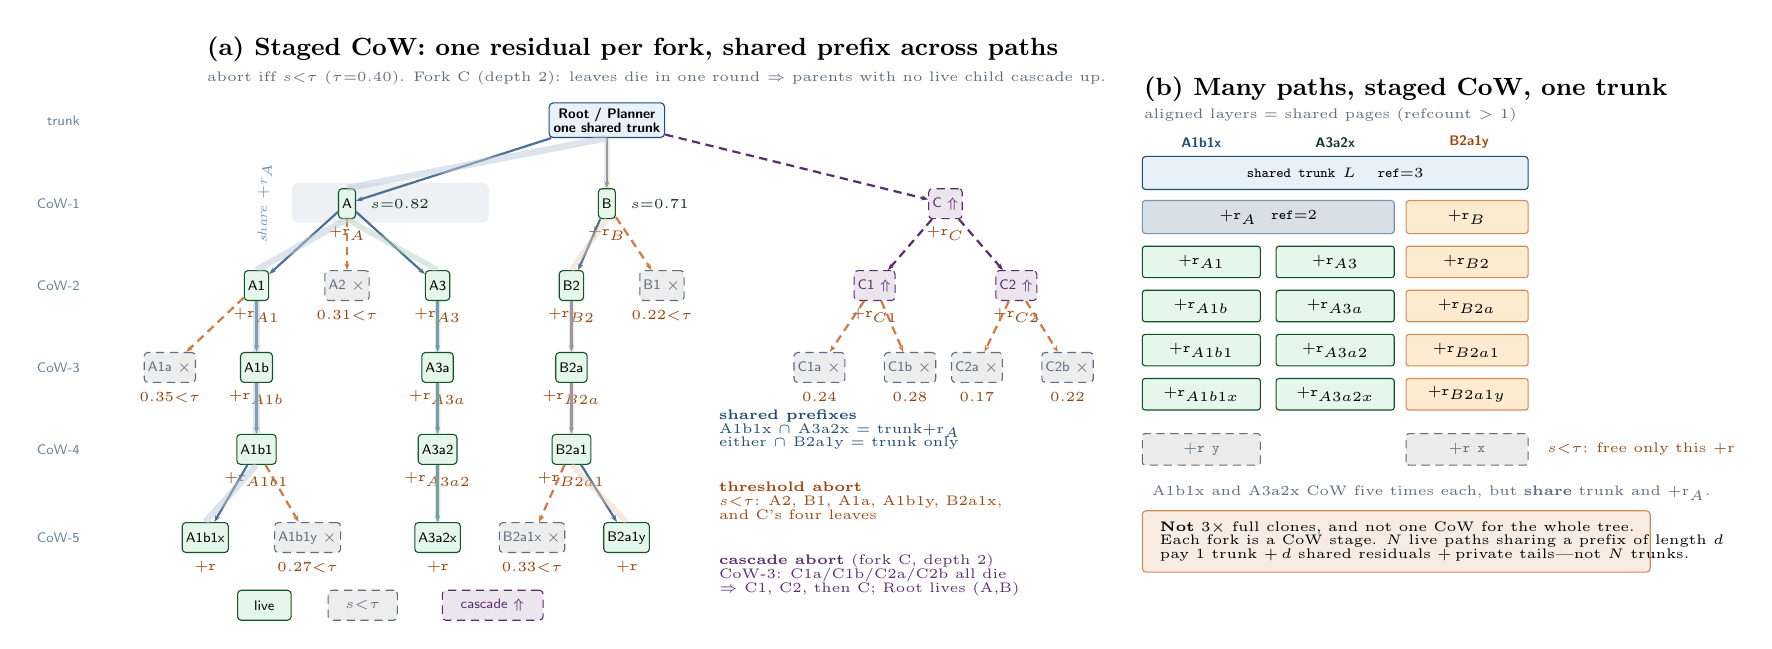
\begin{tikzpicture}[
  font=\scriptsize,
  >=Stealth,
  live/.style={draw=fsgreen!70!black, fill=fscommit, rounded corners=1.3pt,
               inner sep=1.3pt, align=center, font=\tiny\sffamily, minimum height=0.38cm},
  dead/.style={draw=fsgray, fill=black!7, rounded corners=1.3pt, densely dashed,
               inner sep=1.3pt, align=center, font=\tiny\sffamily, minimum height=0.38cm, text=fsgray},
  casc/.style={draw=fspurple, fill=fspurple!12, rounded corners=1.3pt, densely dashed,
               inner sep=1.3pt, align=center, font=\tiny\sffamily, minimum height=0.38cm, text=fspurple},
  root/.style={draw=fsblue, fill=fslight, rounded corners=1.5pt,
               inner sep=1.6pt, align=center, font=\tiny\sffamily\bfseries, minimum height=0.44cm},
  arr/.style={-{Stealth[length=2.4pt,width=1.8pt]}, thick, fsblue!80},
  darr/.style={-{Stealth[length=2.4pt,width=1.8pt]}, thick, densely dashed, fsorange!80},
  carr/.style={-{Stealth[length=2.4pt,width=1.8pt]}, thick, densely dashed, fspurple},
  rlab/.style={font=\tiny\ttfamily, text=fsorange!80!black},
  sc/.style={font=\tiny, text=fsgreen!40!black},
  sd/.style={font=\tiny, text=fsorange!75!black},
  stg/.style={font=\tiny\sffamily, text=fsblue!70, align=right, anchor=east},
]
% ============================================================
% (a)
% ============================================================
\node[font=\small\bfseries, anchor=west] at (-0.35,6.28) {(a) Staged CoW: one residual per fork, shared prefix across paths};
\node[font=\tiny, text=fsgray, anchor=west] at (-0.35,5.92)
  {abort iff $s{<}\tau$ ($\tau{=}0.40$). Fork C (depth 2): leaves die in one round $\Rightarrow$ parents with no live child cascade up.};

% stage labels
\node[stg] at (-1.72,5.38) {trunk};
\node[stg] at (-1.72,4.32) {CoW-1};
\node[stg] at (-1.72,3.28) {CoW-2};
\node[stg] at (-1.72,2.24) {CoW-3};
\node[stg] at (-1.72,1.20) {CoW-4};
\node[stg] at (-1.72,0.08) {CoW-5};

\node[root] (R) at (4.85,5.38) {Root / Planner \\[-1pt]{\tiny one shared trunk}};

% CoW-1: A, B, and cascade root C
\node[live] (A) at (1.55,4.32) {A};
\node[live] (B) at (4.85,4.32) {B};
\node[casc] (C) at (9.15,4.32) {C $\Uparrow$};
\node[rlab] at (1.55,3.94) {$+$r$_A$};
\node[rlab] at (4.85,3.94) {$+$r$_B$};
\node[rlab] at (9.15,3.94) {$+$r$_C$};
\node[sc] at (2.22,4.32) {$s{=}0.82$};
\node[sc] at (5.52,4.32) {$s{=}0.71$};

% CoW-2
\node[live] (A1) at (0.40,3.28) {A1};
\node[dead] (A2) at (1.55,3.28) {A2 $\times$};
\node[live] (A3) at (2.70,3.28) {A3};
\node[live] (B2) at (4.40,3.28) {B2};
\node[dead] (B1) at (5.55,3.28) {B1 $\times$};
\node[casc] (C1) at (8.25,3.28) {C1 $\Uparrow$};
\node[casc] (C2) at (10.05,3.28) {C2 $\Uparrow$};
\node[rlab] at (0.40,2.90) {$+$r$_{A1}$};
\node[rlab] at (2.70,2.90) {$+$r$_{A3}$};
\node[rlab] at (4.40,2.90) {$+$r$_{B2}$};
\node[sd] at (1.55,2.90) {$0.31{<}\tau$};
\node[sd] at (5.55,2.90) {$0.22{<}\tau$};
\node[rlab] at (8.25,2.90) {$+$r$_{C1}$};
\node[rlab] at (10.05,2.90) {$+$r$_{C2}$};

% CoW-3: original plus C's depth-2 leaves (all die this round)
\node[dead] (A1a) at (-0.70,2.24) {A1a $\times$};
\node[live] (A1b) at (0.40,2.24) {A1b};
\node[live] (A3a) at (2.70,2.24) {A3a};
\node[live] (B2a) at (4.40,2.24) {B2a};
\node[dead] (C1a) at (7.55,2.24) {C1a $\times$};
\node[dead] (C1b) at (8.70,2.24) {C1b $\times$};
\node[dead] (C2a) at (9.55,2.24) {C2a $\times$};
\node[dead] (C2b) at (10.70,2.24) {C2b $\times$};
\node[rlab] at (0.40,1.86) {$+$r$_{A1b}$};
\node[rlab] at (2.70,1.86) {$+$r$_{A3a}$};
\node[rlab] at (4.40,1.86) {$+$r$_{B2a}$};
\node[sd] at (-0.70,1.86) {$0.35{<}\tau$};
\node[sd] at (7.55,1.86) {$0.24$};
\node[sd] at (8.70,1.86) {$0.28$};
\node[sd] at (9.55,1.86) {$0.17$};
\node[sd] at (10.70,1.86) {$0.22$};

% CoW-4
\node[live] (A1b1) at (0.40,1.20) {A1b1};
\node[live] (A3a2) at (2.70,1.20) {A3a2};
\node[live] (B2a1) at (4.40,1.20) {B2a1};
\node[rlab] at (0.40,0.82) {$+$r$_{A1b1}$};
\node[rlab] at (2.70,0.82) {$+$r$_{A3a2}$};
\node[rlab] at (4.40,0.82) {$+$r$_{B2a1}$};

% CoW-5
\node[live] (A1b1x) at (-0.25,0.08) {A1b1x};
\node[dead] (A1b1y) at (1.05,0.08) {A1b1y $\times$};
\node[live] (A3a2x) at (2.70,0.08) {A3a2x};
\node[dead] (B2a1x) at (3.90,0.08) {B2a1x $\times$};
\node[live] (B2a1y) at (5.10,0.08) {B2a1y};
\node[rlab] at (-0.25,-0.30) {$+$r};
\node[sd] at (1.05,-0.30) {$0.27{<}\tau$};
\node[rlab] at (2.70,-0.30) {$+$r};
\node[sd] at (3.90,-0.30) {$0.33{<}\tau$};
\node[rlab] at (5.10,-0.30) {$+$r};

\draw[arr] (R) -- (A);
\draw[arr] (R) -- (B);
\draw[carr] (R) -- (C);
\draw[arr] (A) -- (A1);
\draw[darr] (A) -- (A2);
\draw[arr] (A) -- (A3);
\draw[arr] (B) -- (B2);
\draw[darr] (B) -- (B1);
\draw[carr] (C) -- (C1);
\draw[carr] (C) -- (C2);
\draw[darr] (A1) -- (A1a);
\draw[arr] (A1) -- (A1b);
\draw[arr] (A3) -- (A3a);
\draw[arr] (B2) -- (B2a);
\draw[darr] (C1) -- (C1a);
\draw[darr] (C1) -- (C1b);
\draw[darr] (C2) -- (C2a);
\draw[darr] (C2) -- (C2b);
\draw[arr] (A1b) -- (A1b1);
\draw[arr] (A3a) -- (A3a2);
\draw[arr] (B2a) -- (B2a1);
\draw[arr] (A1b1) -- (A1b1x);
\draw[darr] (A1b1) -- (A1b1y);
\draw[arr] (A3a2) -- (A3a2x);
\draw[darr] (B2a1) -- (B2a1x);
\draw[arr] (B2a1) -- (B2a1y);

\begin{scope}[on background layer]
  \fill[fsblue!8, rounded corners=2pt] (0.85,4.08) rectangle (3.35,4.58);
  \node[font=\tiny\itshape, text=fsblue!60, rotate=90, anchor=south] at (0.72,4.33) {share $+$r$_A$};
\end{scope}

\draw[fsblue!30, line width=2.4pt, opacity=0.5]
  (R.south) -- (A.north)
  (A.south) -- (A1.north)
  (A1.south) -- (A1b.north)
  (A1b.south) -- (A1b1.north)
  (A1b1.south) -- (A1b1x.north);
\draw[fsgreen!35, line width=2.0pt, opacity=0.45]
  (A.south) -- (A3.north)
  (A3.south) -- (A3a.north)
  (A3a.south) -- (A3a2.north)
  (A3a2.south) -- (A3a2x.north);
\draw[fsorange!30, line width=2.0pt, opacity=0.45]
  (R.south) -- (B.north)
  (B.south) -- (B2.north)
  (B2.south) -- (B2a.north)
  (B2a.south) -- (B2a1.north)
  (B2a1.south) -- (B2a1y.north);

\node[font=\tiny, text=fsblue, align=left, anchor=west] at (6.15,1.45)
  {\textbf{shared prefixes}\\[-1pt]
   A1b1x $\cap$ A3a2x $=$ trunk${+}$r$_A$\\[-1pt]
   either $\cap$ B2a1y $=$ trunk only};
\node[font=\tiny, text=fsorange!80!black, align=left, anchor=west] at (6.15,0.55)
  {\textbf{threshold abort}\\[-1pt]
   $s{<}\tau$: A2, B1, A1a, A1b1y, B2a1x,\\[-1pt]
   and C's four leaves};
\node[font=\tiny, text=fspurple, align=left, anchor=west] at (6.15,-0.40)
  {\textbf{cascade abort} (fork C, depth 2)\\[-1pt]
   CoW-3: C1a/C1b/C2a/C2b all die\\[-1pt]
   $\Rightarrow$ C1, C2, then C; Root lives (A,B)};

\node[live, minimum width=0.68cm] at (0.50,-0.78) {live};
\node[dead, minimum width=0.88cm] at (1.75,-0.78) {$s{<}\tau$};
\node[casc, minimum width=1.28cm] at (3.40,-0.78) {cascade $\Uparrow$};

% ============================================================
% (b)
% ============================================================
\begin{scope}[shift={(11.55,-0.78)}]
  \node[font=\small\bfseries, anchor=west] at (0,6.55) {(b) Many paths, staged CoW, one trunk};
  \node[font=\tiny, text=fsgray, anchor=west] at (0,6.22)
    {aligned layers $=$ shared pages (refcount $>$ 1)};

  \node[font=\tiny\sffamily\bfseries, text=fsblue] at (0.85,5.88) {A1b1x};
  \node[font=\tiny\sffamily\bfseries, text=fsgreen!50!black] at (2.55,5.88) {A3a2x};
  \node[font=\tiny\sffamily\bfseries, text=fsorange!80!black] at (4.25,5.88) {B2a1y};

  \fill[fslight, draw=fsblue, rounded corners=1.2pt] (0.10,5.28) rectangle (5.00,5.70);
  \node[font=\tiny\ttfamily] at (2.55,5.49) {shared trunk $L$ \quad ref${=}3$};

  \fill[fsblue!18, draw=fsblue!60, rounded corners=1.1pt] (0.10,4.72) rectangle (3.30,5.14);
  \node[font=\tiny\ttfamily] at (1.70,4.93) {$+$r$_A$ \ ref${=}2$};
  \fill[fsspec, draw=fsorange!70, rounded corners=1.1pt] (3.45,4.72) rectangle (5.00,5.14);
  \node[font=\tiny\ttfamily] at (4.22,4.93) {$+$r$_B$};

  \foreach \y/\la/\lb/\lc in {
    4.16/{$+$r$_{A1}$}/{$+$r$_{A3}$}/{$+$r$_{B2}$},
    3.60/{$+$r$_{A1b}$}/{$+$r$_{A3a}$}/{$+$r$_{B2a}$},
    3.04/{$+$r$_{A1b1}$}/{$+$r$_{A3a2}$}/{$+$r$_{B2a1}$},
    2.48/{$+$r$_{A1b1x}$}/{$+$r$_{A3a2x}$}/{$+$r$_{B2a1y}$}} {
    \fill[fscommit, draw=fsgreen!65!black, rounded corners=1.0pt]
      (0.10,\y) rectangle (1.60,\y+0.40);
    \node[font=\tiny\ttfamily] at (0.85,\y+0.20) {\la};
    \fill[fscommit, draw=fsgreen!65!black, rounded corners=1.0pt]
      (1.80,\y) rectangle (3.30,\y+0.40);
    \node[font=\tiny\ttfamily] at (2.55,\y+0.20) {\lb};
    \fill[fsspec, draw=fsorange!70, rounded corners=1.0pt]
      (3.45,\y) rectangle (5.00,\y+0.40);
    \node[font=\tiny\ttfamily] at (4.22,\y+0.20) {\lc};
  }

  \fill[black!8, draw=fsgray, densely dashed, rounded corners=1.0pt]
    (0.10,1.78) rectangle (1.60,2.18);
  \node[font=\tiny\ttfamily, text=fsgray] at (0.85,1.98) {$+$r y};
  \fill[black!8, draw=fsgray, densely dashed, rounded corners=1.0pt]
    (3.45,1.78) rectangle (5.00,2.18);
  \node[font=\tiny\ttfamily, text=fsgray] at (4.22,1.98) {$+$r x};
  \node[font=\tiny, text=fsorange!80!black, anchor=west] at (5.12,1.98)
    {$s{<}\tau$: free only this $+$r};

  \node[font=\tiny, text=fsgray, anchor=west, align=left] at (0.10,1.42)
    {A1b1x and A3a2x CoW five times each, but \textbf{share} trunk and $+$r$_A$.};

  \fill[fsorange!12, draw=fsorange!70, rounded corners=1.4pt]
    (0.10,0.42) rectangle (6.55,1.20);
  \node[font=\tiny, anchor=west, align=left] at (0.20,0.81)
    {\textbf{Not} 3$\times$ full clones, and not one CoW for the whole tree.\\[-1pt]
     Each fork is a CoW stage. $N$ live paths sharing a prefix of length $d$\\[-1pt]
     pay $1$ trunk $+\,d$ shared residuals $+\,$private tails---not $N$ trunks.};
\end{scope}
\end{tikzpicture}
\vspace{-0.35em}
}
\caption{\textbf{Staged CoW along many paths, threshold abort, cascade abort, shared prefixes.}
(a)~Each edge is one CoW: the child aliases the parent's pages and allocates only a residual ($+$r).
Live paths A1b1x, A3a2x, and B2a1y share the trunk; the first two also share $+$r$_A$.
Fork C has depth 2: at CoW-3 all four leaves die, so abort cascades through C1 and C2, then C; it stops at Root, which still has live children A and B.
(b)~KV stacks of the three live leaves, layers aligned: a shared layer is one physical page set with refcount ${>}1$, not $N$ copies.
Aborting A1b1y or B2a1x frees only that leaf residual; cascade-aborting C also frees $+$r$_{C1}$, $+$r$_{C2}$, and $+$r$_C$.}
\label{fig:tree}
\end{figure*}

\paragraph{Action.}
Let $H$ be the published radix index and $P$ the page size.
The matched prefix, the loop set, and the early-abort bit are
\begin{align}
m_i &= \max\{jP: jP\le\ell_i,\;\rho_i[0{:}jP)\in H\}, \label{eq:mi}\\
\Lambda &= \{i\neq 0:\mathrm{Loop}(\rho_i)\}, \nonumber\\
F_i &= \bigl[s\bigl(\rho_i[0{:}\lceil\alpha\ell_i\rceil]\bigr)<\tau\bigr]. \nonumber
\end{align}
The trunk is the alias $\sigma_i\leftarrow(\sigma_u,|x_u|)$, so $L\notin\Work_i$.
With $\Act=\{\mathrm{HS},\mathrm{HP},\mathrm{DS},\mathrm{EA},\mathrm{PF}\}$ and first-match Iverson brackets,
\begin{equation}
\label{eq:action}
\begin{aligned}
a_i &= \mathrm{HS}[m_i{=}\ell_i]
+\mathrm{HP}[0{<}m_i{<}\ell_i]
+\mathrm{DS}[m_i{=}0][i{\in}\Lambda]\\
&\quad+\mathrm{EA}[m_i{=}0][i{\notin}\Lambda][F_i]
+\mathrm{PF}[m_i{=}0][i{\notin}\Lambda][\neg F_i].
\end{aligned}
\end{equation}
Index $0$ is forced into $\Keep$, and $a_0\in\{\mathrm{HS},\mathrm{HP},\mathrm{PF}\}$.
\begin{align}
\Work_i &= \lceil\alpha\ell_i\rceil[a_i{=}\mathrm{EA}]+(\ell_i{-}m_i)[a_i{=}\mathrm{HP}]+\ell_i[a_i{=}\mathrm{PF}], \label{eq:work}\\
\Xfer_i &= \Work_i\,[i{\in}\Keep]\,[a_i{\in}\{\mathrm{HP},\mathrm{PF}\}]. \label{eq:xfer}
\end{align}
\Cref{fig:radix} is \eqref{eq:action}--\eqref{eq:xfer} on one radix tree: green pages lie in $H$, orange pages are grown, gray pages are withheld.

\begin{figure*}[t]
\centering
\resizebox{\textwidth}{!}{% One radix tree. Five edges are the five actions.
% Green = page in H. Orange = grown by prefill. Gray = withheld.
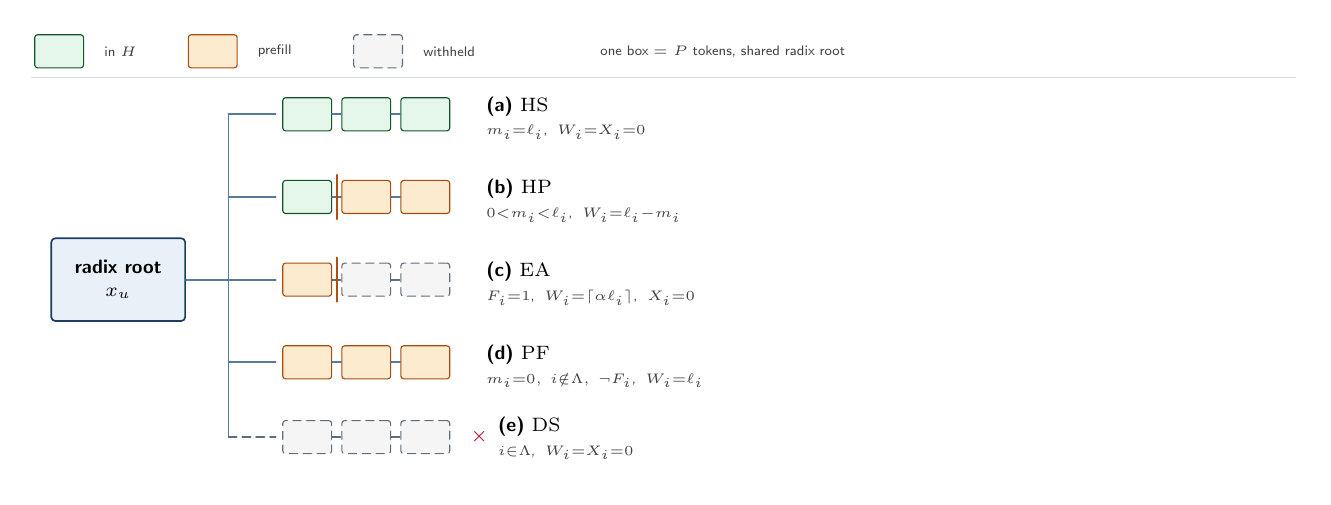
\begin{tikzpicture}[
  x=1cm, y=1cm,
  font=\sffamily,
  >=Stealth,
  line cap=round, line join=round,
  root/.style={draw=fsblue!80!black, fill=fslight, rounded corners=1.4pt, line width=0.6pt,
    align=center, font=\scriptsize\sffamily\bfseries, inner sep=3pt,
    minimum width=1.7cm, minimum height=1.05cm},
  pg/.style={draw, rounded corners=1pt, minimum width=0.62cm, minimum height=0.42cm,
    inner sep=0pt, font=\tiny\ttfamily, line width=0.4pt},
  inH/.style={pg, draw=fsgreen!70!black, fill=fscommit},
  pref/.style={pg, draw=fsorange!85!black, fill=fsspec},
  hold/.style={pg, draw=fsgray, fill=black!4, densely dashed},
  edge/.style={line width=0.65pt, draw=fsblue!75},
  dashE/.style={edge, densely dashed, draw=fsgray},
  lab/.style={font=\scriptsize\sffamily\bfseries, anchor=west},
  meta/.style={font=\tiny\sffamily, anchor=west, text=black!75},
  cut/.style={draw=fsorange!90!black, line width=0.75pt},
]
\path (0,-0.15) rectangle (16.2,5.55);

\node[inH] at (0.40,5.25) {};
\node[meta] at (0.85,5.25) {in $H$};
\node[pref] at (2.35,5.25) {};
\node[meta] at (2.80,5.25) {prefill};
\node[hold] at (4.45,5.25) {};
\node[meta] at (4.90,5.25) {withheld};
\node[meta] at (7.15,5.25) {one box $=P$ tokens, shared radix root};
\draw[fsblue!20, line width=0.3pt] (0.05,4.92) -- (16.10,4.92);

\node[root] (R) at (1.15,2.35) {radix root\\$x_u$};

% vertical bus of the radix tree
\draw[edge] (R.east) -- (2.55,2.35);
\draw[edge] (2.55,4.45) -- (2.55,0.35);

% row helper: #1 y, #2 label, #3 formula, then three page styles and edge styles drawn by hand

% (a) HS
\draw[edge] (2.55,4.45) -- (3.15,4.45);
\node[inH] (a1) at (3.55,4.45) {};
\node[inH] (a2) at (4.30,4.45) {};
\node[inH] (a3) at (5.05,4.45) {};
\draw[edge] (a1) -- (a2) -- (a3);
\node[lab] at (5.70,4.55) {(a)\ $\mathrm{HS}$};
\node[meta] at (5.70,4.22) {$m_i{=}\ell_i$,\ \ $\Work_i{=}\Xfer_i{=}0$};

% (b) HP
\draw[edge] (2.55,3.40) -- (3.15,3.40);
\node[inH] (b1) at (3.55,3.40) {};
\node[pref] (b2) at (4.30,3.40) {};
\node[pref] (b3) at (5.05,3.40) {};
\draw[edge] (b1) -- (b2);
\draw[edge] (b2) -- (b3);
\coordinate (kb) at ($(b1.east)!0.5!(b2.west)$);
\draw[cut] ($(kb)+(0,-0.28)$) -- ($(kb)+(0,0.28)$);
\node[lab] at (5.70,3.50) {(b)\ $\mathrm{HP}$};
\node[meta] at (5.70,3.17) {$0{<}m_i{<}\ell_i$,\ \ $\Work_i{=}\ell_i{-}m_i$};

% (c) EA
\draw[edge] (2.55,2.35) -- (3.15,2.35);
\node[pref] (c1) at (3.55,2.35) {};
\node[hold] (c2) at (4.30,2.35) {};
\node[hold] (c3) at (5.05,2.35) {};
\draw[dashE] (c1) -- (c2) -- (c3);
\coordinate (kc) at ($(c1.east)!0.5!(c2.west)$);
\draw[cut] ($(kc)+(0,-0.28)$) -- ($(kc)+(0,0.28)$);
\node[lab] at (5.70,2.45) {(c)\ $\mathrm{EA}$};
\node[meta] at (5.70,2.12) {$F_i{=}1$,\ \ $\Work_i{=}\lceil\alpha\ell_i\rceil$,\ \ $\Xfer_i{=}0$};

% (d) PF
\draw[edge] (2.55,1.30) -- (3.15,1.30);
\node[pref] (d1) at (3.55,1.30) {};
\node[pref] (d2) at (4.30,1.30) {};
\node[pref] (d3) at (5.05,1.30) {};
\draw[edge] (d1) -- (d2) -- (d3);
\node[lab] at (5.70,1.40) {(d)\ $\mathrm{PF}$};
\node[meta] at (5.70,1.07) {$m_i{=}0,\ i{\notin}\Lambda,\ \neg F_i$,\ \ $\Work_i{=}\ell_i$};

% (e) DS
\draw[dashE] (2.55,0.35) -- (3.15,0.35);
\node[hold] (e1) at (3.55,0.35) {};
\node[hold] (e2) at (4.30,0.35) {};
\node[hold] (e3) at (5.05,0.35) {};
\draw[dashE] (e1) -- (e2) -- (e3);
\node[font=\scriptsize\sffamily\bfseries, text=fsred, anchor=west] at (5.50,0.35) {$\times$};
\node[lab] at (5.85,0.48) {(e)\ $\mathrm{DS}$};
\node[meta] at (5.85,0.15) {$i{\in}\Lambda$,\ \ $\Work_i{=}\Xfer_i{=}0$};
\end{tikzpicture}
}
\caption{\textbf{One radix tree, five actions} (\eqref{eq:action}--\eqref{eq:xfer}).
The root is the aliased trunk $x_u$.
Each edge is one page of $P$ tokens.
Green pages are in $H$; orange pages are prefilled; gray pages are withheld.
(a)~$\mathrm{HS}$: $m_i{=}\ell_i$, $\Work_i{=}\Xfer_i{=}0$.
(b)~$\mathrm{HP}$: $0{<}m_i{<}\ell_i$, $\Work_i{=}\ell_i{-}m_i$.
(c)~$\mathrm{EA}$: $m_i{=}0$, $F_i{=}1$, $\Work_i{=}\lceil\alpha\ell_i\rceil$, $\Xfer_i{=}0$.
(d)~$\mathrm{PF}$: $m_i{=}0$, $i{\notin}\Lambda$, $\neg F_i$, $\Work_i{=}\ell_i$.
(e)~$\mathrm{DS}$: $i{\in}\Lambda$, $\Work_i{=}\Xfer_i{=}0$.
A score below $\tau$ with $i{\notin}\Lambda$ is prefilled and probed (\Cref{alg:app}).}
\label{fig:radix}
\end{figure*}
\begin{equation}
\label{eq:drej}
d_i^{\times}=D\cdot[i=0\lor s_i\ge\tau].
\end{equation}
\eqref{eq:drej} drops every $s_i{<}\tau$ before prefill.
\Cref{alg:app} keeps $\mathrm{DS}$ only for $i{\in}\Lambda$; every other low score is prefilled and probed.
\Cref{tab:span} is the resulting first-expand span.

\begin{algorithm}[t]
\caption{Probe admission, replacing \eqref{eq:drej}.
$\Lambda$ is the repeated-loop set.
$y_i$ is a probe of $t_0$ tokens and $s'_i$ is its draft score.
Iverson brackets select the decode length.
$\mathrm{DS}$ applies only to $\Lambda$.}
\label{alg:app}
\small
\begin{algorithmic}[1]
\REQUIRE $\{\rho_i\}_{i=0}^{k-1}$, threshold $\tau$, probe $t_0$, budget $D$
\ENSURE action $a_i$, decode length $d_i$, set $\Keep$
\STATE $\Lambda\leftarrow\{i\neq 0:\mathrm{Loop}(\rho_i)\}$
\FOR{$i=0$ \TO $k-1$}
  \STATE $s_i\leftarrow\mathrm{DraftScore}(\rho_i)$
  \IF{$i\in\Lambda$}
    \STATE $(a_i,d_i)\leftarrow(\mathrm{DS},\,0)$ \COMMENT{\eqref{eq:drej} set $d_i^{\times}{=}0$ for all $s_i{<}\tau$}
  \ELSIF{$i=0 \lor s_i\ge\tau$}
    \STATE $(a_i,d_i)\leftarrow(\mathrm{PF},\,D)$
  \ELSE
    \STATE $y_i\leftarrow\mathrm{Dec}(x_u\Vert\rho_i,\,t_0)$
    \STATE $s'_i\leftarrow\mathrm{DraftScore}(y_i)$
    \STATE $(a_i,d_i)\leftarrow\big(\mathrm{PF},\; D[s'_i\ge\tau]+t_0[s'_i<\tau]\big)$
  \ENDIF
\ENDFOR
\STATE $\Keep\leftarrow\{i:a_i\neq\mathrm{DS}\}$
\STATE $\Work_i\leftarrow\ell_i\cdot[a_i=\mathrm{PF}]$
\STATE $\mathrm{DecTokens}\leftarrow\sum_{i=0}^{k-1} d_i$
\end{algorithmic}
\end{algorithm}

\begin{table*}[t]
\centering
\caption{Work, transfer, and memory spans (bottleneck in \textcolor{fsred}{red}).
$W_{\mathrm{pre}}$ is GPU prefill tokens; $X$ is connector tokens; $M$ is live KV after abort;
$T_{\mathrm{ab}}$ is abort cost in pages; replay is a later \texttt{open} of the published winner.
$\mathrm{PAR}$ is the number of trunk copies touched on the first expand.}
\label{tab:span}
\scriptsize
\setlength{\tabcolsep}{3.2pt}
\setlength{\aboverulesep}{0.4pt}
\setlength{\belowrulesep}{0.4pt}
\begin{tabular}{@{}lcccccc@{}}
\rowcolor{tblhead}
\toprule
 & $W_{\mathrm{pre}}$ & $X$ & $M$ after abort & $T_{\mathrm{ab}}$ & $\mathrm{PAR}_{\mathrm{trunk}}$ & Replay $W_{\mathrm{pre}}$ \\
\midrule
Recompute & \botn{$kL+\sum_i\ell_i$} & $0$ & \botn{$kL+\sum_i\ell_i$} & $\Theta(kL/P)$ & $k$ & $kL+\ell_\star$ \\
\rowcolor{tblalt}
APC (first expand) & \botn{$kL+\sum_i\ell_i$} & $0$ & $kL+\sum_i\ell_i$ & LRU of hashed $\rho$ & $k$ & $0$ \\
hash prefill (first) & \botn{$kL+\sum_i\ell_i$} & $0$ & $kL+\sum_i\ell_i$ & LRU & $k$ & $0$ \\
\rowcolor{tblalt}
P/D disagg. & \botn{$kL+\sum_i\ell_i$} & \botn{$kL+\sum_i\ell_i$} & $kL+\sum_i\ell_i$ & full KV transfer & $k$ & $0$ \\
FS CoW & $L+\sum_i\ell_i$ & $0$ & \win{$L+\ell_\star$} & $\Theta(\ell_i/P)$ & $1$ & $L_{\mathrm{miss}}$ \\
\rowcolor{tblalt}
FS+ + P/D & \win{$L+\sum_{i\in\Keep}\ell_i$} & \win{$\sum_{i\in\Keep}\Work_i$} & \win{$L+\ell_\star$} & lazy, residual only & $1$ & \win{$0$} \\
% FS+ + stop & $L+\sum_{i\in\Keep}\ell_i$ & $\sum_{i\in\Keep}\Work_i$ & \win{$L+\ell_\star$} & lazy & $1$ & $0$ \\
\bottomrule
\end{tabular}

\vspace{0.25em}
{\scriptsize
$P{=}16$.
Known-suffix items ($p{=}1$) are admitted before residuals ($p{<}1$).
Spec pages are never hashed; LCP commit publishes full blocks of $x_\star$.
% Decode stop changes $D^{+}$, not $W_{\mathrm{pre}}$.
}
\end{table*}

\begin{lemma}[First-fan-out dominance]
\label{lem:dom}
On a cold index, $\Work_{\mathrm{APP}}\le\Work_{\mathrm{CoW}}\le\Work_{\mathrm{APC}}=\Work_{\mathrm{PD}}$ and $\Xfer_{\mathrm{APP}}\le\Xfer_{\mathrm{PD}}$, with strict inequality in $\Work$ whenever at least one repeated loop is draft-skipped, and strict inequality in $\Xfer$ whenever $\Keep\neq[k]$ or any kept residual is a hash hit.
\end{lemma}

\paragraph{From the action to the wire.}
The index key is $\mathrm{hash}(\mathrm{parent},\;\mathrm{block\_tokens},\;\mathrm{extra})$~\cite{vllm}, and only full pages enter $H$, so $m_i$ in \eqref{eq:mi} steps by $P$.
\eqref{eq:lcp} is what later sets $m_i{=}\ell_i$.
A hit is already visible on the decoder, hence $\Xfer_i{=}0$ when $a_i{=}\mathrm{HS}$.
\eqref{eq:drej} withholds every $s_i{<}\tau$; \Cref{alg:app} restricts that withhold to $i{\in}\Lambda$ and continues any other low score past $t_0$ iff $s'_i{\ge}\tau$.
The $t_0$ probe is a decode prefix; $F_i$ is a prefill prefix.
Defaults are $\tau_{\mathrm{pre}}{=}0.15$, and on MATH-500 $\tau{=}0.45$, $t_0{\in}\{64,128\}$.
Baseline disaggregation moves \eqref{eq:xfer-stock}; the rule moves \eqref{eq:xfer}.
\begin{equation}
\label{eq:tfan}
T_{\mathrm{fan}}=\Pref(\Work)+\mu\,\Xfer+T_{\mathrm{CoW}}+T_{\mathrm{abort}}.
\end{equation}
$T_{\mathrm{CoW}}$ is a pointer swap.
\S\ref{sec:eval-app} evaluates \eqref{eq:drej} at $139$\,ms (APC), $162$\,ms (baseline disaggregation), $47$\,ms (alias only), and $31.4$\,ms.
\S\ref{sec:eval-prefill} uses \Cref{alg:app} and cuts computed prefill by $23\%$.

\iffalse
\paragraph{Orthogonal decode-length stop.}
The cascade changes $\Work$ and $M$.
End-to-end time is still $T_{\mathrm{fan}}+T_{\mathrm{dec}}(D)$, so a shorter prefill does not by itself shorten decode.
ForkServe+ stops committed decode only when the last non-empty line is a finished answer (\texttt{\#\#\#\#} or a closed \texttt{\textbackslash boxed}).
An earlier \texttt{\#\#\#\#} is an intermediate step, and a bare \texttt{</think>} is not an answer.
If item $j$ hits a marker at $t_j$, emitted tokens are $D^{+}=\sum_j\min(t_j,D)\le nD$, and $T_{\mathrm{dec}}$ scales with $D^{+}$ when decode is memory-bandwidth bound.
The stop ends a finished answer; it does not draft output tokens, and it does not change which residual was admitted.
\fi

\subsection{Critical-Path Placement}
\label{sec:schedule}
Abort under the rule leaves $M_{\mathrm{spine}}=b(L+\ell_\star)$, so the same pool admits
\begin{equation}
\label{eq:slots}
C=\bigl\lfloor H/M\bigr\rfloor
\end{equation}
sessions, with $M=M_{\mathrm{spine}}$ for \sys and $M=M_{\mathrm{APC}}$ while a prefix cache still holds aborted residuals.
\begin{equation}
\label{eq:theta}
\Theta\;\propto\; C/T_{\mathrm{e2e}}.
\end{equation}
On tick $t$ the chunk budget~\cite{sarathi} splits by the committed rate $\underline{s}_r$~\cite{jitserve},
\begin{align}
B^{\mathrm{c}}_t &= \min\Bigl(B_t,\; \sum_{r\in R^{\mathrm{c}}_t}\max(\underline{s}_r\Delta,\;1)\Bigr), \label{eq:bc}\\
B^{\mathrm{s}}_t &= B_t-B^{\mathrm{c}}_t. \label{eq:bs}
\end{align}
$B^{\mathrm{c}}_t$ decodes the spine.
$B^{\mathrm{s}}_t$ prefills the next miss tail, or a known suffix ($p{=}1$) when $\Pref(|w|)\le\Idle(u)$.
The observation then pays only the unmatched tail under \eqref{eq:lcp}.
Speculative tokens stay outside the sampler.

\section{Evaluation}
\label{sec:eval}

The GPU measurements share one node and one engine, and they differ by model, tensor-parallel width, and workload.
\S\ref{sec:eval-gpu} is the full GSM8K forest on Qwen3-14B at $\mathrm{tp}{=}2$.
\S\ref{sec:eval-app} is the earlier blanket-skip cost model of \app, with no GPU, against APC, hash prefill, baseline prefill--decode disaggregation, \sys, and three decoding-time pruners; \S\ref{sec:eval-grow} replaces that skip.
\S\ref{sec:eval-prefill} measures the GSM8K prefill threshold $\tau_{\mathrm{pre}}{=}0.15$ on Qwen3-8B and the accuracy--latency trade-off when that rule sits in front of ESC, Speculative Rejection, and DPTS.
\S\ref{sec:eval-plus} runs ForkServe+ on Qwen3-8B at $\mathrm{tp}{=}2$ and $\mathrm{tp}{=}4$.
\S\ref{sec:eval-mt} is a three-turn Tree-of-Thoughts on Qwen3-4B and Qwen3-8B, one problem per generate.
\S\ref{sec:eval-multi} repeats the forest on six families at $n{=}40$.
\S\ref{sec:eval-sens} sweeps branching, depth, pruning, and batch width on Llama-3-8B, Mistral-7B, and DeepSeek-R1-Distill-Llama-8B, then runs a $2048$-token contest forest on that DeepSeek model and on Qwen3-4B.

\paragraph{Setup.}
GPU runs use vLLM on four A100-SXM4 40GB GPUs, with \texttt{bfloat16} weights and $\mathrm{tp}{=}2$ or $4$.
The models are Qwen3-14B, Qwen3-8B, Qwen3-4B, Qwen2.5-Math-1.5B, Llama-3-8B, Mistral-7B, and DeepSeek-R1-Distill-Llama-8B.
Tree-of-Thoughts uses $k{=}4$ and a $512$-token budget ($2048$ on the contest forest), in batches of eight.
The three-turn run in \S\ref{sec:eval-mt} issues one problem per generate.
A math answer is correct when its final number matches the reference.

\subsection{GPU forest}
\label{sec:eval-gpu}

\paragraph{Setup.}
This section uses Qwen3-14B at $\mathrm{tp}{=}2$.
The GSM8K test set has $1319$ problems.
Each problem is expanded with four thoughts and decoded for at most $512$ tokens, in $165$ batches of eight.
Accuracy is the fraction of problems whose final number matches the reference.

\begin{table}[t]
\centering
\caption{GSM8K test, Qwen3-14B, $\mathrm{tp}{=}2$, $n{=}1319$.
Median over $165$ batches of eight.
Best storage in green.}
\label{tab:gsm}
\scriptsize
\setlength{\tabcolsep}{3.5pt}
\setlength{\aboverulesep}{0.4pt}
\setlength{\belowrulesep}{0.4pt}
\begin{tabular}{lrrr}
\rowcolor{tblhead}
\toprule
 & recompute & APC & FS \\
\midrule
Accuracy & $0.847$ & $0.844$ & $0.845$ \\
\rowcolor{tblalt}
Peak KV, median (tok) & $4136$ & $1430$ & \win{$1030$} \\
Peak KV, max (tok) & $4944$ & $1632$ & \win{$1232$} \\
\rowcolor{tblalt}
Peak / APC & $2.89\times$ & $1.00\times$ & \win{$0.72\times$} \\
Fan-out, median (ms) & $326$ & $87$ & $140$ \\
\rowcolor{tblalt}
Generation (min) & --- & $18.6$ & $18.9$ \\
KV saving vs.\ rec. & --- & $0.65$ & \win{$0.75$} \\
\bottomrule
\end{tabular}
\end{table}

\paragraph{Storage and expand latency.}
\Cref{tab:gsm} reports the storage result and the expand-latency gap that \app is designed to close.
Median peak KV is $0.72\times$ APC and $0.25\times$ recompute, and accuracy stays within one point of both.
Storage and fan-out do not share that ordering: median fan-out is $140$\,ms for \sys and $87$\,ms for APC, because copy-on-write and abort execute on the expand path, whereas an APC hash hit does not.
End-to-end generation remains within $2\%$ of APC ($18.9$ vs.\ $18.6$ minutes).
The same peak ordering, $0.58$--$0.80\times$ APC, holds on seven math sets for Qwen3-14B, Qwen3-8B, and DeepSeek-R1-Distill-Llama-8B at $\mathrm{tp}{=}2$ and $\mathrm{tp}{=}4$.
The peak is unchanged when the tensor width doubles; it follows the committed path, as \eqref{eq:mem} requires.

\subsection{Prefill pruning}
\label{sec:eval-app}

\paragraph{Setup.}
This subsection is the earlier blanket-skip cost model, not the GPU rule of \S\ref{sec:eval-grow,sec:eval-prefill}.
Control plane, no GPU.
Ten sessions, $k{=}4$, $L{=}256$, $\ell{=}32$.
Two of four residuals fail the draft score and are withheld before prefill; the winner is index $0$.
Prefill time is $\ell\times 12\,\mu\mathrm{s}/\mathrm{token}$; P/D transfer is $2\,\mu\mathrm{s}/\mathrm{token}$.
APC and hash prefill publish blocks only after a request materializes them, so the first fan-out clones $k$ trunks.
Baseline disaggregation uses that prefill and then transfers the live token span.
\sys aliases the trunk by pointer swap and prefills the $k$ residuals.
\app adds hash skip, draft prune, early abort, lazy abort, and a connector that inserts only retained residuals.

\begin{table}[t]
\centering
\caption{Control-plane fan-out ($10$ sessions, $k{=}4$, $L{=}256$, $\ell{=}32$).
Bottleneck in red; ForkServe+ in green.
Not GPU wall-clock.}
\label{tab:app}
\scriptsize
\setlength{\tabcolsep}{2.2pt}
\setlength{\aboverulesep}{0.35pt}
\setlength{\belowrulesep}{0.35pt}
\begin{tabular}{llrrrrrr}
\rowcolor{tblhead}
\toprule
Phase & Method & $W$ & $T_{\mathrm{fan}}$ & $X$ & peak & skip & prune \\
\midrule
\multirow{5}{*}{fan-out}
 & APC & \botn{$11520$} & $139.0$ & $0$ & $11520$ & $0$ & $0$ \\
\rowcolor{tblalt}
 & hash & \botn{$11520$} & $139.0$ & $0$ & $11520$ & $0$ & $0$ \\
 & P/D disagg. & \botn{$11520$} & \botn{$162.1$} & \botn{$11520$} & $11520$ & $0$ & $0$ \\
\rowcolor{tblalt}
 & FS & $3840$ & $47.1$ & $0$ & $3840$ & $0$ & $0$ \\
 & ForkServe+ & \win{$2592$} & \win{$31.4$} & \win{$32$} & \win{$2880$} & $9$ & $30$ \\
\midrule
 & ForkServe+ / APC & \win{$-77.5\%$} & \win{$-77.4\%$} & --- & \win{$-75\%$} & --- & --- \\
\bottomrule
\end{tabular}
\end{table}

\paragraph{Fan-out.}
\Cref{tab:app} is the comparison the GPU gap motivates.
% and \Cref{fig:eval-stack} shows occupancy over the expand--abort--decode phase.
On the first expand, hash prefill matches APC: the blocks are unpublished, so the hash probe does not remove the cloned trunks.
Baseline disaggregation exceeds APC ($162$ vs.\ $139$\,ms) because it transfers that clone.
\sys removes the clone by aliasing the trunk ($3840$ prefill tokens, $47$\,ms).
\app then withholds prefill from $30$ of the $40$ residuals, which reduces $T_{\mathrm{fan}}$ to $31.4$\,ms and the connector payload from $11520$ tokens to $32$.

\paragraph{Decoding-time pruning.}
\Cref{tab:decode-prune} runs ESC~\cite{esc}, Speculative Rejection~\cite{specrej}, and DPTS~\cite{dpts} on this same fan-out.
Each method prefills the shared trunk once.
The length of the decode that produces the prune score is the length published for that method.
ESC stops after a window of $5$ agreeing samples; this fan-out has four children and two low-score answers, so the window stays open and every child is decoded to the $512$-token budget.
Speculative Rejection is charged its partial-reward horizon $\tau{=}256$ and then drops the lower half ($\alpha{=}0.5$); the memory-limit trigger in that paper would not fire at $k{=}4$, so $\tau$ is the earlier checkpoint.
DPTS early-stops after its $100$-token mini-step.
The two low-score children are the ones removed, and the winner is kept.
Decoded tokens use the same $12\,\mu\mathrm{s}/\mathrm{token}$ clock.
DPTS is the earliest cut of the three and still decodes $4000$ tokens before the drop, $2000$ of them on losers, reaching the cut at $78.7$\,ms.
\app has already withheld those residuals: $0$ tokens on losers and $T_{\mathrm{fan}}{=}31.4$\,ms.
That row is the blanket skip.
\S\ref{sec:eval-grow} replaces it: only a repeated loop is withheld before prefill.

\begin{table}[t]
\centering
\caption{Decoding-time pruning on the \Cref{tab:app} fan-out ($10{\times}4$, $L{=}256$).
Decode-to-cut is the prefix that must be generated before a child can be dropped.
``On losers'' counts that prefix on the two low-score children.
Same $12\,\mu\mathrm{s}/\mathrm{token}$ clock. Not GPU wall-clock.}
\label{tab:decode-prune}
\scriptsize
\setlength{\tabcolsep}{3.2pt}
\setlength{\aboverulesep}{0.4pt}
\setlength{\belowrulesep}{0.4pt}
\begin{tabular}{lrrrrr}
\rowcolor{tblhead}
\toprule
 & prefill & decode & on losers & peak & $T_{\mathrm{cut}}$ \\
\midrule
ESC & $2560$ & \botn{$20480$} & \botn{$10240$} & \botn{$23040$} & \botn{$276.5$} \\
\rowcolor{tblalt}
Spec.\ Rejection & $2560$ & $10240$ & $5120$ & $12800$ & $153.6$ \\
DPTS & $2560$ & $4000$ & $2000$ & $6560$ & $78.7$ \\
\rowcolor{tblalt}
ForkServe+ & $2592$ & \win{$0$} & \win{$0$} & \win{$2880$} & \win{$31.4$} \\
\bottomrule
\end{tabular}
\end{table}

% Temporarily omitted from the paper (Figure 4, stacked KV occupancy).
\iffalse
\begin{figure*}[t]
\centering
\resizebox{\textwidth}{!}{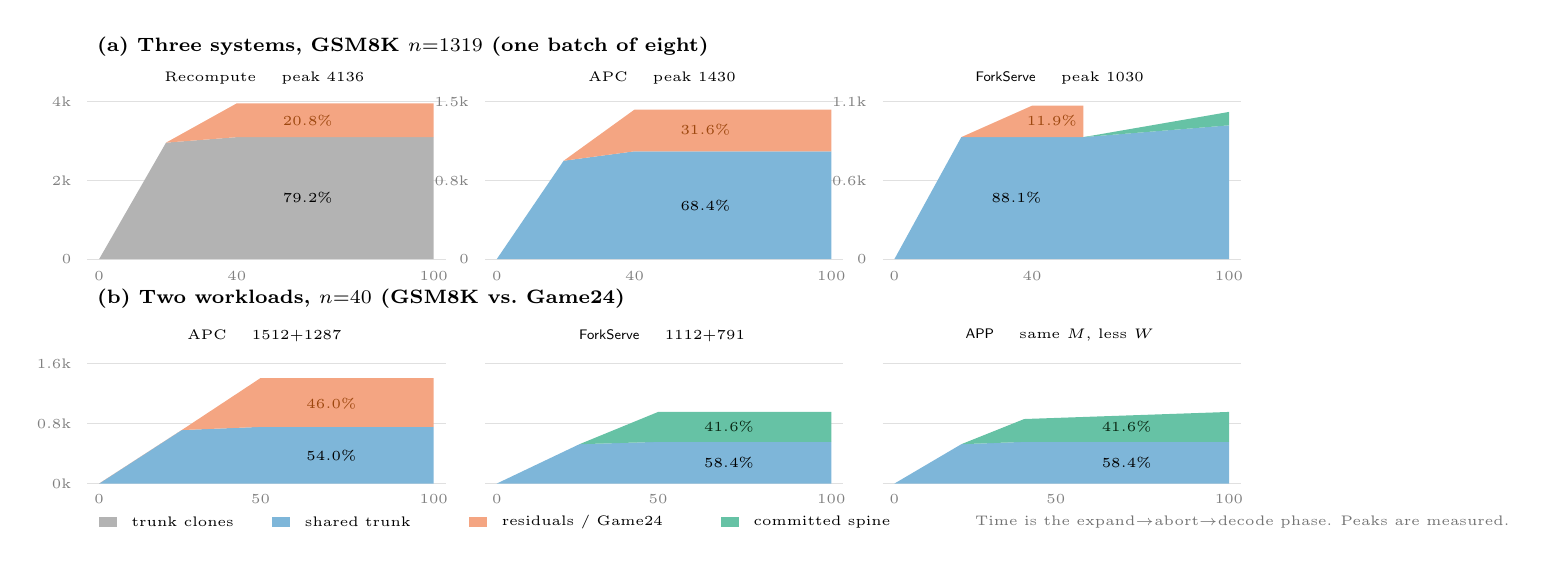
\begin{tikzpicture}[
  font=\scriptsize\sffamily,
  >=Latex,
]
\definecolor{Tr}{HTML}{7EB6D9}
\definecolor{Rs}{HTML}{F4A582}
\definecolor{Sp}{HTML}{66C2A5}
\definecolor{Cl}{HTML}{B3B3B3}

% Stacked occupancy over a batch. y-scale in tokens (GPU medians / control-plane shape).
% Time: 0 open, 20 fork, 40 prefill, 60 abort, 80--100 decode.
% (a) three systems on GSM8K 14B (measured peak: rec 4136, APC 1430, FS 1030).
% (b) two workloads at n=40 (GSM8K APC 1512 / FS 1112; Game24 APC 1287 / FS 791).

% ---- helper: one stacked panel ----
% We inline 6 panels.

% ===== (a) =====
\node[font=\scriptsize\bfseries, anchor=west] at (0,5.55) {(a) Three systems, GSM8K $n{=}1319$ (one batch of eight)};

% Per-panel y-scale so each stack fills (reference style). Peak is in the title.
% -- Recompute, max 4.2k → 2.00cm --
\begin{scope}[shift={(0,2.85)}]
  \foreach \y/\lab in {0/0, 2.1/2k, 4.2/4k} {
    \draw[black!12] (0,\y*0.476) -- (4.55,\y*0.476);
    \node[font=\tiny, text=black!50, anchor=east] at (-0.08,\y*0.476) {\lab};
  }
  \fill[Cl] (0.15,0) -- (1.00,1.48) -- (1.90,1.55) -- (4.40,1.55) -- (4.40,0) -- cycle;
  \fill[Rs] (1.00,1.48) -- (1.90,1.98) -- (4.40,1.98) -- (4.40,1.55) -- (1.90,1.55) -- cycle;
  \node[font=\tiny] at (2.80,0.78) {$79.2\%$};
  \node[font=\tiny, text=fsorange!80!black] at (2.80,1.76) {$20.8\%$};
  \foreach \x/\lab in {0.15/0, 1.90/40, 4.40/100} {
    \node[font=\tiny, text=black!50] at (\x,-0.22) {\lab};
  }
  \node[font=\tiny, anchor=south] at (2.25,2.10) {Recompute \quad peak $4136$};
\end{scope}

% -- APC, max 1.50k → 2.00cm --
\begin{scope}[shift={(5.05,2.85)}]
  \foreach \y/\lab in {0/0, 0.75/0.8k, 1.50/1.5k} {
    \draw[black!12] (0,\y*1.333) -- (4.55,\y*1.333);
    \node[font=\tiny, text=black!50, anchor=east] at (-0.08,\y*1.333) {\lab};
  }
  \fill[Tr] (0.15,0) -- (1.00,1.25) -- (1.90,1.37) -- (4.40,1.37) -- (4.40,0) -- cycle;
  \fill[Rs] (1.00,1.25) -- (1.90,1.90) -- (4.40,1.90) -- (4.40,1.37) -- (1.90,1.37) -- cycle;
  \node[font=\tiny] at (2.80,0.68) {$68.4\%$};
  \node[font=\tiny, text=fsorange!80!black] at (2.80,1.64) {$31.6\%$};
  \foreach \x/\lab in {0.15/0, 1.90/40, 4.40/100} {
    \node[font=\tiny, text=black!50] at (\x,-0.22) {\lab};
  }
  \node[font=\tiny, anchor=south] at (2.25,2.10) {APC \quad peak $1430$};
\end{scope}

% -- FS, max 1.10k → 2.00cm --
\begin{scope}[shift={(10.10,2.85)}]
  \foreach \y/\lab in {0/0, 0.55/0.6k, 1.10/1.1k} {
    \draw[black!12] (0,\y*1.818) -- (4.55,\y*1.818);
    \node[font=\tiny, text=black!50, anchor=east] at (-0.08,\y*1.818) {\lab};
  }
  \fill[Tr] (0.15,0) -- (1.00,1.55) -- (1.90,1.55) -- (2.55,1.55) -- (4.40,1.70) -- (4.40,0) -- cycle;
  \fill[Rs] (1.00,1.55) -- (1.90,1.95) -- (2.55,1.95) -- (2.55,1.55) -- cycle;
  \fill[Sp] (2.55,1.55) -- (4.40,1.87) -- (4.40,1.70) -- cycle;
  \node[font=\tiny] at (1.70,0.78) {$88.1\%$};
  \node[font=\tiny, text=fsorange!80!black] at (2.15,1.76) {$11.9\%$};
  \foreach \x/\lab in {0.15/0, 1.90/40, 4.40/100} {
    \node[font=\tiny, text=black!50] at (\x,-0.22) {\lab};
  }
  \node[font=\tiny, anchor=south] at (2.25,2.10) {\sys{} \quad peak $1030$};
\end{scope}

% ===== (b) =====
\node[font=\scriptsize\bfseries, anchor=west] at (0,2.35) {(b) Two workloads, $n{=}40$ (GSM8K vs.\ Game24)};

% GSM8K APC vs FS stacked as two systems in one panel? Reference has 3 schedulers.
% Three panels: APC / FS / FS+ for GSM8K (left cluster) is too many.
% Do: GSM8K (APC+FS overlay stacked) | Game24 (APC+FS) | mix percentages
% Cleaner: three panels APC, FS, FS+ but only two workloads as two stacked hues? 
% Match reference: 3 panels = APC, FS, APP; each stacks GSM8K (bottom) + Game24 (top) as two "models"

\begin{scope}[shift={(0,0)}]
  \foreach \y in {0,0.8,1.6} {
    \draw[black!12] (0,\y*0.95) -- (4.55,\y*0.95);
    \node[font=\tiny, text=black!50, anchor=east] at (-0.08,\y*0.95) {\y k};
  }
  % APC: GSM8K 1.51 + Game24 1.29 as stacked share of a 2-workload mix
  % Show occupancy of GSM8K (bottom teal) and Game24 (top orange) under APC
  \fill[Tr] (0.15,0) -- (1.20,0.68) -- (2.20,0.72) -- (4.40,0.72) -- (4.40,0) -- cycle;
  \fill[Rs] (0.15,0) -- (1.20,0.68) -- (2.20,1.34) -- (4.40,1.34) -- (4.40,0.72) -- (2.20,0.72) -- (1.20,0.68) -- cycle;
  \node[font=\tiny] at (3.10,0.36) {$54.0\%$};
  \node[font=\tiny, text=fsorange!80!black] at (3.10,1.02) {$46.0\%$};
  \foreach \x/\lab in {0.15/0, 2.20/50, 4.40/100} {
    \node[font=\tiny, text=black!50] at (\x,-0.20) {\lab};
  }
  \node[font=\tiny, anchor=south] at (2.25,1.68) {APC \quad $1512{+}1287$};
\end{scope}

\begin{scope}[shift={(5.05,0)}]
  \foreach \y in {0,0.8,1.6} {
    \draw[black!12] (0,\y*0.95) -- (4.55,\y*0.95);
  }
  \fill[Tr] (0.15,0) -- (1.20,0.50) -- (2.20,0.53) -- (4.40,0.53) -- (4.40,0) -- cycle;
  \fill[Sp] (1.20,0.50) -- (2.20,0.91) -- (4.40,0.91) -- (4.40,0.53) -- (2.20,0.53) -- cycle;
  \node[font=\tiny] at (3.10,0.26) {$58.4\%$};
  \node[font=\tiny, text=fsgreen!30!black] at (3.10,0.72) {$41.6\%$};
  \foreach \x/\lab in {0.15/0, 2.20/50, 4.40/100} {
    \node[font=\tiny, text=black!50] at (\x,-0.20) {\lab};
  }
  \node[font=\tiny, anchor=south] at (2.25,1.68) {\sys{} \quad $1112{+}791$};
\end{scope}

\begin{scope}[shift={(10.10,0)}]
  \foreach \y in {0,0.8,1.6} {
    \draw[black!12] (0,\y*0.95) -- (4.55,\y*0.95);
  }
  % APP same M as FS (1112+791) but residuals drop earlier
  \fill[Tr] (0.15,0) -- (1.00,0.50) -- (1.80,0.53) -- (4.40,0.53) -- (4.40,0) -- cycle;
  \fill[Sp] (1.00,0.50) -- (1.80,0.82) -- (4.40,0.91) -- (4.40,0.53) -- (1.80,0.53) -- cycle;
  \node[font=\tiny] at (3.10,0.26) {$58.4\%$};
  \node[font=\tiny, text=fsgreen!30!black] at (3.10,0.72) {$41.6\%$};
  \foreach \x/\lab in {0.15/0, 2.20/50, 4.40/100} {
    \node[font=\tiny, text=black!50] at (\x,-0.20) {\lab};
  }
  \node[font=\tiny, anchor=south] at (2.25,1.68) {\app{} \quad same $M$, less $\Work$};
\end{scope}

% legend
\fill[Cl] (0.15,-0.55) rectangle (0.38,-0.42);
\node[font=\tiny, anchor=west] at (0.44,-0.485) {trunk clones};
\fill[Tr] (2.35,-0.55) rectangle (2.58,-0.42);
\node[font=\tiny, anchor=west] at (2.64,-0.485) {shared trunk};
\fill[Rs] (4.85,-0.55) rectangle (5.08,-0.42);
\node[font=\tiny, anchor=west] at (5.14,-0.485) {residuals / Game24};
\fill[Sp] (8.05,-0.55) rectangle (8.28,-0.42);
\node[font=\tiny, anchor=west] at (8.34,-0.485) {committed spine};
\node[font=\tiny, text=black!55, anchor=west] at (11.15,-0.485)
  {Time is the expand$\rightarrow$abort$\rightarrow$decode phase. Peaks are measured.};
\end{tikzpicture}
}
\caption{\textbf{Stacked KV occupancy} over the expand$\rightarrow$abort$\rightarrow$decode phase.
(a)~One GSM8K batch of eight on Qwen3-14B (per-panel $y$-scale; peaks $4136$ / $1430$ / $1030$).
Annotated fractions are trunk vs.\ residual under the $k{=}4$, $L{=}256$, $\ell{=}32$ model.
(b)~Two workloads ($n{=}40$): GSM8K (bottom) plus Game24 (top) for APC, \sys, and \app.
\sys{} and \app{} share $M$; \app{} drops residual $\Work$ earlier.
Percentages are the share of the stacked live tokens.}
\label{fig:eval-stack}
\end{figure*}
\fi

\paragraph{Probe-then-grow.}
\label{sec:eval-grow}
The blanket skip is the wrong cut once the residual is not a loop.
We measure the rule in \Cref{alg:app} on Qwen3-8B, one GPU each, four A100-40GB, $\mathrm{tp}{=}1$.
The slice is the first $32$ MATH-500 problems at level $4$ or $5$.
Temperature is $0$, EOS is ignored, prefix caching is on, and the decode budget is $D{=}1024$.
Half of the $k$ residuals are contest strategies.
The other half alternates a repeated loop with illegal text.
A question counts when some branch that ran all $1024$ tokens matches the gold answer.
The winner is residual $0$.

\begin{table}[t]
\centering
\caption{MATH-500 level $\ge 4$, Qwen3-8B, $n{=}32$, $D{=}1024$.
Any-finished is exact match on a branch that ran the full budget.
``Drop $s{<}\tau$'' withholds every low-score residual before prefill.
``Grow $t_0$'' is \Cref{alg:app}: loops stay at $d_i{=}0$; every other low-score residual is probed for $t_0$ tokens and continues to $D$ only if $s'_i\ge\tau{=}0.45$.
Time is trunk warm plus fan-out, in seconds.}
\label{tab:grow}
\scriptsize
\setlength{\tabcolsep}{3.0pt}
\setlength{\aboverulesep}{0.4pt}
\setlength{\belowrulesep}{0.4pt}
\begin{tabular}{lrrr}
\rowcolor{tblhead}
\toprule
 & $k{=}4$ & $k{=}8$ & $k{=}16$ \\
\midrule
Full fan-out & $12/32$, $25.3$ & $15/32$, $52.5$ & $20/32$, $104.1$ \\
\rowcolor{tblalt}
Drop $s{<}\tau$ & $6/32$, $19.1$ & $11/32$, $25.6$ & $13/32$, $52.1$ \\
Skip loops only & $11/32$, $23.0$ & $17/32$, $41.5$ & $16/32$, $71.4$ \\
\rowcolor{tblalt}
Grow $t_0{=}64$ & $8/32$, $24.0$ & \win{$16/32$}, $42.0$ & $18/32$, $72.5$ \\
Grow $t_0{=}128$ & $9/32$, $24.7$ & $13/32$, $43.3$ & \win{$20/32$}, $72.2$ \\
\bottomrule
\end{tabular}
\end{table}

\Cref{tab:grow} is the correction.
Dropping every residual below $\tau$ cuts any-finished from $12/32$ to $6/32$ at $k{=}4$ and from $20/32$ to $13/32$ at $k{=}16$.
Loop branches are $0$ for $0$ at every $k$, so skipping them before prefill is safe.
At $k{=}16$, a $128$-token probe extends every illegal residual ($128/128$) and none of the loops.
Any-finished returns to the full fan-out, $20/32$, while end-to-end time falls from $104.1$\,s to $72.2$\,s and decode tokens from $524288$ to $393216$.
Probing the loops as well extends none of them and costs $74.4$\,s for the same $20/32$.
At $k{=}8$ the shorter probe is the one that holds accuracy: grow at $P{=}64$ is $16/32$ in $42.0$\,s, against $15/32$ in $52.5$\,s for the full fan-out.
At $k{=}4$ the probe does not recover the full fan-out ($9/32$ against $12/32$); skipping the single loop, and decoding the illegal residual to $D$, is $11/32$ in $23.0$\,s.

\paragraph{Accuracy--speed trade-off.}
\label{sec:eval-prefill}
The MATH-500 probe still uses a decode threshold $\tau{=}0.45$ on the generated prefix.
Prefill admission is a different score, with default $\tau_{\mathrm{pre}}{=}0.15$: it drops only the repeated loop ($0.02$) and starts illegal text ($0.22$) and every live strategy ($1.0$).
We measure that rule on Qwen3-8B GSM8K, $n{=}16$, $D{=}512$, the same hopeless mix, four A100-40GB, $\mathrm{tp}{=}1$.
The host decoder is ESC, so a withheld child never pays residual prefill or a decode slot.
A denser sweep of $\tau_{\mathrm{pre}}$ collapses to three admission sets; $0.15$ and $0.45$ are the two nonzero operating points.

\begin{table}[t]
\centering
\caption{GSM8K, Qwen3-8B, $n{=}16$, $D{=}512$, ESC only.
Any-finished is exact match on a full-budget branch.
$\tau_{\mathrm{pre}}{=}0.15$ drops the loop; $0.45$ also drops illegal text.
Time is trunk warm plus fan-out, in seconds.
Computed prefill falls $23\%$ at $0.15$ and $45\%$ at $0.45$ at every $k$.}
\label{tab:prefill-bar}
\scriptsize
\setlength{\tabcolsep}{3.0pt}
\setlength{\aboverulesep}{0.4pt}
\setlength{\belowrulesep}{0.4pt}
\begin{tabular}{lrrr}
\rowcolor{tblhead}
\toprule
 & $k{=}4$ & $k{=}8$ & $k{=}16$ \\
\midrule
ESC & $16/16$, $8.65$ & $16/16$, $10.84$ & $16/16$, $17.05$ \\
\rowcolor{tblalt}
\app $\tau_{\mathrm{pre}}{=}0.15$ & $15/16$, $8.22$ & \win{$16/16$}, $10.19$ & \win{$16/16$}, $14.14$ \\
\app $\tau_{\mathrm{pre}}{=}0.45$ & \botn{$14/16$}, $7.89$ & \botn{$14/16$}, $8.60$ & \win{$16/16$}, \win{$10.93$} \\
\bottomrule
\end{tabular}
\end{table}

\Cref{tab:prefill-bar} is the trade-off.
$\tau_{\mathrm{pre}}{=}0.15$ keeps $15/16$, $16/16$, $16/16$ and still cuts wall-clock time, more as the tree widens ($-5\%$, $-6\%$, $-17\%$).
Computed prefill tokens fall from $1320/2624/5008$ to $1018/2020/3848$.
Raising $\tau_{\mathrm{pre}}$ to $0.45$ is the extra-speed point: $-9\%$, $-21\%$, $-36\%$ end-to-end, and $732/1448/2768$ computed prefill tokens.
It drops two questions at $k{=}4$ and $k{=}8$.
At $k{=}16$ both thresholds stay at $16/16$, so $0.45$ is the faster matched-accuracy setting ($10.93$\,s vs.\ $14.14$\,s).
The default is $0.15$ because it holds accuracy at every $k$.

\begin{table}[t]
\centering
\caption{Same GSM8K slice, $k{=}16$, $\tau_{\mathrm{pre}}{=}0.15$ in front of three host decoders.
Admitted children and computed prefill tokens are identical across hosts: prefill admission does not read $\tau$, $d_{\mathrm{DPTS}}$, or $\alpha$.
Any-finished stays $16/16$.}
\label{tab:plugin}
\scriptsize
\setlength{\tabcolsep}{3.2pt}
\setlength{\aboverulesep}{0.4pt}
\setlength{\belowrulesep}{0.4pt}
\begin{tabular}{lrrrr}
\rowcolor{tblhead}
\toprule
 & adm. & prefill & e2e (s) & any \\
\midrule
ESC & $16$ & $5008$ & $17.05$ & $16/16$ \\
\rowcolor{tblalt}
ESC+\app & $12$ & \win{$3848$} & \win{$14.14$} & $16/16$ \\
Spec.\ Rejection & $16$ & $5008$ & $13.14$ & $16/16$ \\
\rowcolor{tblalt}
SR+\app & $12$ & \win{$3848$} & $12.47$ & $16/16$ \\
DPTS & $16$ & $5008$ & $11.86$ & $16/16$ \\
\rowcolor{tblalt}
DPTS+\app & $12$ & \win{$3848$} & $11.49$ & $16/16$ \\
\bottomrule
\end{tabular}
\end{table}

\Cref{tab:plugin} stacks the same $\tau_{\mathrm{pre}}{=}0.15$ in front of each host.
ESC, Speculative Rejection, and DPTS alone all report $5008$ computed prefill tokens: a decode-time cut still prefills every child.
Adding \app admits $12$ of $16$ residuals and $3848$ prefill tokens on every host.
Wall-clock falls $17\%$ on ESC, $5\%$ on Speculative Rejection, and $3\%$ on DPTS, because those last two hosts would have stopped the loop later anyway.
The accuracy that \Cref{tab:prefill-bar} preserves is unchanged: every row in \Cref{tab:plugin} is $16/16$.
At $k{=}8$ the same threshold is $16/16$ on ESC ($10.84$ to $10.19$\,s) and lifts Speculative Rejection and DPTS from $15/16$ to $16/16$.

\paragraph{Concurrency from measured KV.}
Our empirical results on DeepSeek-R1 GSM8K ($761$ APC tokens, $561$ \sys tokens, $n{=}16$, $k{=}4$) in an $8$\,GiB pool in \eqref{eq:theta} give $76$ concurrent trees for APC and $103$ for \sys.
\Cref{fig:eval-slo} sweeps offered QPS: under a $1$\,s P99 \ttft{} constraint the same model admits $384$ QPS for APC and $512$ for the pruned tree, and saturated decode throughput rises from $48640$ to $65920$ tokens/s (\gain{$+35.5\%$}).
This uses measured $M$, not the control-plane peak of \Cref{tab:app}.

\begin{figure}[t]
\centering
\resizebox{\columnwidth}{!}{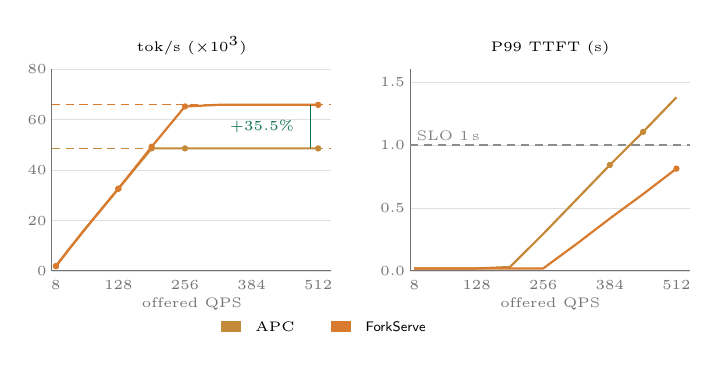
\begin{tikzpicture}[
  font=\scriptsize\sffamily,
  >=Latex,
  tick/.style={font=\tiny, text=black!55, inner sep=0pt},
  grid/.style={black!12, line width=0.25pt},
]
\definecolor{APC}{HTML}{C48A3A}
\definecolor{FSln}{HTML}{D97B2F}

% Measured DeepSeek-R1 GSM8K peaks: APC 761 tok, spine 561 tok.
% 8 GiB pool, 147456 B/token -> C = 76 and 103.
% Service model: e2e = 0.4 s, 256 decode tokens, so one slot is 640 tok/s.
% tok/s = min(round(qps*0.4), C) * 640.
% qps:     8, 32, 64, 128, 192, 256, 320, 384, 448, 512
% APC:  1920, 8320, 16640, 32640, 48640, then 48640
% FS:   1920, 8320, 16640, 32640, 49280, 65280, then 65920
% P99 s, APC: 0.020 until 128, 0.031, 0.294, 0.567, 0.841, 1.104, 1.378
% P99 s, FS:  0.020 until 256, 0.214, 0.416, 0.610, 0.812
% Left y: thousands, 0--80.  x: 512 * 0.0066 = 3.38

\begin{scope}[shift={(0,0)}]
  \foreach \y in {0,20,40,60,80} {
    \draw[grid] (0,\y*0.032) -- (3.55,\y*0.032);
    \node[tick, anchor=east] at (-0.06,\y*0.032) {\y};
  }
  \draw[black!55, line width=0.35pt] (0,0) -- (3.55,0);
  \draw[black!55, line width=0.35pt] (0,0) -- (0,2.56);
  % APC plateau 48.64, spine plateau 65.92
  \draw[APC, densely dashed, line width=0.3pt] (0,48.64*0.032) -- (3.55,48.64*0.032);
  \draw[FSln, densely dashed, line width=0.3pt] (0,65.92*0.032) -- (3.55,65.92*0.032);
  \draw[APC, line width=0.8pt]
    (8*0.0066, 1.92*0.032) -- (32*0.0066, 8.32*0.032) -- (64*0.0066, 16.64*0.032)
    -- (128*0.0066, 32.64*0.032) -- (192*0.0066, 48.64*0.032) -- (512*0.0066, 48.64*0.032);
  \draw[FSln, line width=0.8pt]
    (8*0.0066, 1.92*0.032) -- (32*0.0066, 8.32*0.032) -- (64*0.0066, 16.64*0.032)
    -- (128*0.0066, 32.64*0.032) -- (192*0.0066, 49.28*0.032) -- (256*0.0066, 65.28*0.032)
    -- (320*0.0066, 65.92*0.032) -- (512*0.0066, 65.92*0.032);
  \foreach \q/\ya/\yf in {8/1.92/1.92, 128/32.64/32.64, 192/48.64/49.28, 256/48.64/65.28, 512/48.64/65.92} {
    \fill[APC] (\q*0.0066, \ya*0.032) circle (1.15pt);
    \fill[FSln] (\q*0.0066, \yf*0.032) circle (1.15pt);
  }
  \draw[fsgain, line width=0.4pt] (3.28,48.64*0.032) -- (3.28,65.92*0.032);
  \node[font=\tiny, text=fsgain, anchor=east] at (3.20,1.83) {$+35.5\%$};
  \foreach \q/\lab in {8/8, 128/128, 256/256, 384/384, 512/512} {
    \node[tick] at (\q*0.0066, -0.18) {\lab};
  }
  \node[font=\tiny, anchor=south] at (1.78,2.62) {tok/s ($\times 10^{3}$)};
  \node[tick] at (1.78, -0.42) {offered QPS};
\end{scope}

\begin{scope}[shift={(4.55,0)}]
  \foreach \y in {0.0,0.5,1.0,1.5} {
    \draw[grid] (0,\y*1.60) -- (3.55,\y*1.60);
    \node[tick, anchor=east] at (-0.06,\y*1.60) {\y};
  }
  \draw[black!55, line width=0.35pt] (0,0) -- (3.55,0);
  \draw[black!55, line width=0.35pt] (0,0) -- (0,2.56);
  \draw[black!45, densely dashed] (0,1.60) -- (3.55,1.60);
  \node[tick, anchor=west, text=black!50] at (0.08,1.72) {SLO $1$\,s};
  \draw[APC, line width=0.8pt]
    (8*0.0066, 0.020*1.60) -- (128*0.0066, 0.020*1.60) -- (192*0.0066, 0.031*1.60)
    -- (256*0.0066, 0.294*1.60) -- (320*0.0066, 0.567*1.60) -- (384*0.0066, 0.841*1.60)
    -- (448*0.0066, 1.104*1.60) -- (512*0.0066, 1.378*1.60);
  \draw[FSln, line width=0.8pt]
    (8*0.0066, 0.020*1.60) -- (256*0.0066, 0.020*1.60) -- (320*0.0066, 0.214*1.60)
    -- (384*0.0066, 0.416*1.60) -- (448*0.0066, 0.610*1.60) -- (512*0.0066, 0.812*1.60);
  \fill[APC] (384*0.0066, 0.841*1.60) circle (1.15pt);
  \fill[APC] (448*0.0066, 1.104*1.60) circle (1.15pt);
  \fill[FSln] (512*0.0066, 0.812*1.60) circle (1.15pt);
  \foreach \q/\lab in {8/8, 128/128, 256/256, 384/384, 512/512} {
    \node[tick] at (\q*0.0066, -0.18) {\lab};
  }
  \node[font=\tiny, anchor=south] at (1.78,2.62) {P99 TTFT (s)};
  \node[tick] at (1.78, -0.42) {offered QPS};
\end{scope}

\fill[APC] (2.15,-0.78) rectangle (2.40,-0.64);
\node[font=\tiny, anchor=west] at (2.46,-0.71) {APC};
\fill[FSln] (3.55,-0.78) rectangle (3.80,-0.64);
\node[font=\tiny, anchor=west] at (3.86,-0.71) {\sys};
\end{tikzpicture}
}
\caption{\textbf{SLO sweep} from measured DeepSeek GSM8K peaks.
Left: saturated tok/s plateaus at $C{\times}$decode-rate ($76$ vs.\ $103$ slots).
Right: APC crosses the $1$\,s P99 line at $448$ QPS; \sys{} stays under it through $512$.}
\label{fig:eval-slo}
\end{figure}

\begin{figure*}[t]
\centering
\resizebox{\textwidth}{!}{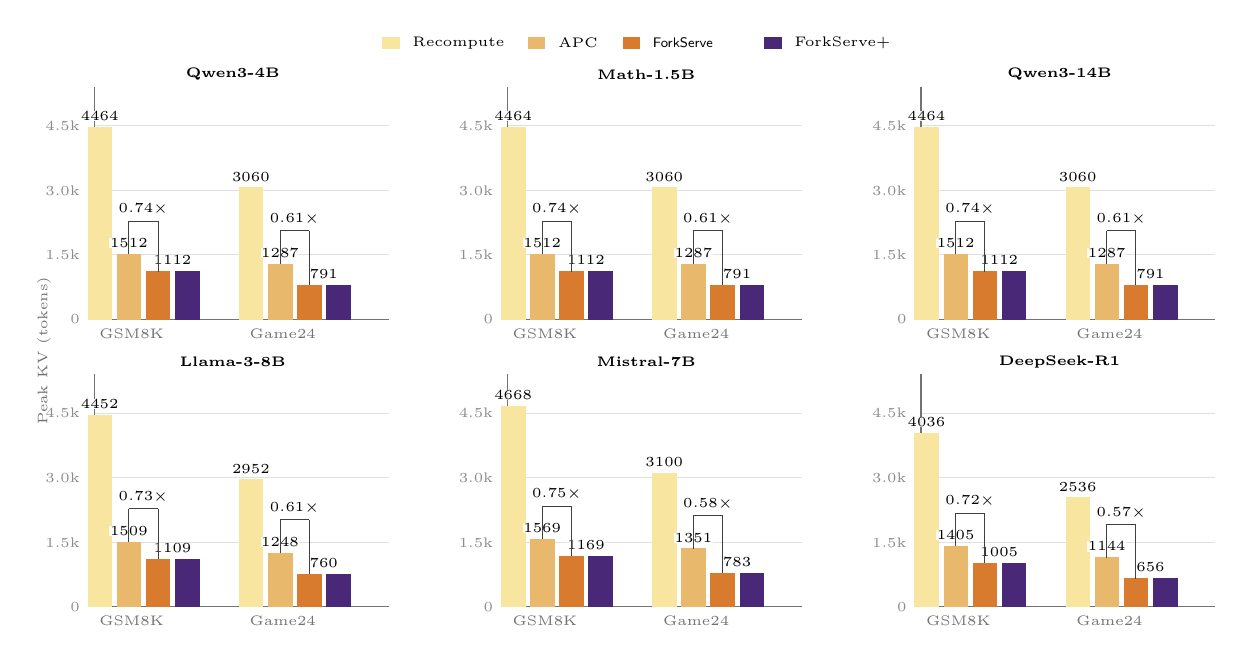
\begin{tikzpicture}[
  font=\scriptsize\sffamily,
  bar/.style={draw=black!65, line width=0.22pt},
  >=Latex,
]
\definecolor{Rec}{HTML}{F8E6A0}
\definecolor{APC}{HTML}{E8B86D}
\definecolor{FS}{HTML}{D97B2F}
\definecolor{FSp}{HTML}{4A2878}

\fill[Rec] (4.10,7.48) rectangle (4.32,7.64);
\node[font=\tiny, anchor=west] at (4.36,7.56) {Recompute};
\fill[APC] (5.95,7.48) rectangle (6.17,7.64);
\node[font=\tiny, anchor=west] at (6.21,7.56) {APC};
\fill[FS] (7.15,7.48) rectangle (7.37,7.64);
\node[font=\tiny, anchor=west] at (7.41,7.56) {\sys};
\fill[FSp] (8.95,7.48) rectangle (9.17,7.64);
\node[font=\tiny, anchor=west] at (9.21,7.56) {ForkServe+};

% --- Qwen3-4B ---
\begin{scope}[shift={(0.00,3.75)}]
  \node[font=\tiny\bfseries] at (2.20,3.41) {Qwen3-4B};
  \draw[black!12] (0.44,0.300) -- (4.18,0.300);
  \node[font=\tiny, text=black!45, anchor=east] at (0.38,0.300) {0};
  \draw[black!12] (0.44,1.119) -- (4.18,1.119);
  \node[font=\tiny, text=black!45, anchor=east] at (0.38,1.119) {1.5k};
  \draw[black!12] (0.44,1.939) -- (4.18,1.939);
  \node[font=\tiny, text=black!45, anchor=east] at (0.38,1.939) {3.0k};
  \draw[black!12] (0.44,2.758) -- (4.18,2.758);
  \node[font=\tiny, text=black!45, anchor=east] at (0.38,2.758) {4.5k};
  \draw[black!55] (0.44,0.30) -- (4.18,0.30);
  \draw[black!55] (0.44,0.30) -- (0.44,3.25);
  \fill[bar, Rec] (0.360,0.30) rectangle (0.660,2.739);
  \fill[bar, APC] (0.730,0.30) rectangle (1.030,1.126);
  \fill[bar, FS] (1.100,0.30) rectangle (1.400,0.907);
  \fill[bar, FSp] (1.470,0.30) rectangle (1.770,0.907);
  \node[font=\tiny, inner sep=0.2pt, fill=white, fill opacity=0.85, text opacity=1] at (0.510,2.879) {4464};
  \node[font=\tiny, inner sep=0.2pt, fill=white, fill opacity=0.85, text opacity=1] at (0.880,1.266) {1512};
  \node[font=\tiny, inner sep=0.2pt, fill=white, fill opacity=0.85, text opacity=1] at (1.435,1.047) {1112};
  \draw[black!75, line width=0.35pt] (0.880,1.126) -- (0.880,1.546);
  \draw[black!75, line width=0.35pt] (0.880,1.546) -- (1.250,1.546);
  \draw[black!75, line width=0.35pt] (1.250,1.546) -- (1.250,0.907);
  \node[font=\tiny\bfseries] at (1.065,1.696) {$0.74\times$};
  \node[font=\tiny, text=black!55] at (0.915,0.12) {GSM8K};
  \fill[bar, Rec] (2.280,0.30) rectangle (2.580,1.972);
  \fill[bar, APC] (2.650,0.30) rectangle (2.950,1.003);
  \fill[bar, FS] (3.020,0.30) rectangle (3.320,0.732);
  \fill[bar, FSp] (3.390,0.30) rectangle (3.690,0.732);
  \node[font=\tiny, inner sep=0.2pt, fill=white, fill opacity=0.85, text opacity=1] at (2.430,2.112) {3060};
  \node[font=\tiny, inner sep=0.2pt, fill=white, fill opacity=0.85, text opacity=1] at (2.800,1.143) {1287};
  \node[font=\tiny, inner sep=0.2pt, fill=white, fill opacity=0.85, text opacity=1] at (3.355,0.872) {791};
  \draw[black!75, line width=0.35pt] (2.800,1.003) -- (2.800,1.423);
  \draw[black!75, line width=0.35pt] (2.800,1.423) -- (3.170,1.423);
  \draw[black!75, line width=0.35pt] (3.170,1.423) -- (3.170,0.732);
  \node[font=\tiny\bfseries] at (2.985,1.573) {$0.61\times$};
  \node[font=\tiny, text=black!55] at (2.835,0.12) {Game24};
\end{scope}

% --- Math-1.5B ---
\begin{scope}[shift={(5.25,3.75)}]
  \node[font=\tiny\bfseries] at (2.20,3.41) {Math-1.5B};
  \draw[black!12] (0.44,0.300) -- (4.18,0.300);
  \node[font=\tiny, text=black!45, anchor=east] at (0.38,0.300) {0};
  \draw[black!12] (0.44,1.119) -- (4.18,1.119);
  \node[font=\tiny, text=black!45, anchor=east] at (0.38,1.119) {1.5k};
  \draw[black!12] (0.44,1.939) -- (4.18,1.939);
  \node[font=\tiny, text=black!45, anchor=east] at (0.38,1.939) {3.0k};
  \draw[black!12] (0.44,2.758) -- (4.18,2.758);
  \node[font=\tiny, text=black!45, anchor=east] at (0.38,2.758) {4.5k};
  \draw[black!55] (0.44,0.30) -- (4.18,0.30);
  \draw[black!55] (0.44,0.30) -- (0.44,3.25);
  \fill[bar, Rec] (0.360,0.30) rectangle (0.660,2.739);
  \fill[bar, APC] (0.730,0.30) rectangle (1.030,1.126);
  \fill[bar, FS] (1.100,0.30) rectangle (1.400,0.907);
  \fill[bar, FSp] (1.470,0.30) rectangle (1.770,0.907);
  \node[font=\tiny, inner sep=0.2pt, fill=white, fill opacity=0.85, text opacity=1] at (0.510,2.879) {4464};
  \node[font=\tiny, inner sep=0.2pt, fill=white, fill opacity=0.85, text opacity=1] at (0.880,1.266) {1512};
  \node[font=\tiny, inner sep=0.2pt, fill=white, fill opacity=0.85, text opacity=1] at (1.435,1.047) {1112};
  \draw[black!75, line width=0.35pt] (0.880,1.126) -- (0.880,1.546);
  \draw[black!75, line width=0.35pt] (0.880,1.546) -- (1.250,1.546);
  \draw[black!75, line width=0.35pt] (1.250,1.546) -- (1.250,0.907);
  \node[font=\tiny\bfseries] at (1.065,1.696) {$0.74\times$};
  \node[font=\tiny, text=black!55] at (0.915,0.12) {GSM8K};
  \fill[bar, Rec] (2.280,0.30) rectangle (2.580,1.972);
  \fill[bar, APC] (2.650,0.30) rectangle (2.950,1.003);
  \fill[bar, FS] (3.020,0.30) rectangle (3.320,0.732);
  \fill[bar, FSp] (3.390,0.30) rectangle (3.690,0.732);
  \node[font=\tiny, inner sep=0.2pt, fill=white, fill opacity=0.85, text opacity=1] at (2.430,2.112) {3060};
  \node[font=\tiny, inner sep=0.2pt, fill=white, fill opacity=0.85, text opacity=1] at (2.800,1.143) {1287};
  \node[font=\tiny, inner sep=0.2pt, fill=white, fill opacity=0.85, text opacity=1] at (3.355,0.872) {791};
  \draw[black!75, line width=0.35pt] (2.800,1.003) -- (2.800,1.423);
  \draw[black!75, line width=0.35pt] (2.800,1.423) -- (3.170,1.423);
  \draw[black!75, line width=0.35pt] (3.170,1.423) -- (3.170,0.732);
  \node[font=\tiny\bfseries] at (2.985,1.573) {$0.61\times$};
  \node[font=\tiny, text=black!55] at (2.835,0.12) {Game24};
\end{scope}

% --- Qwen3-14B ---
\begin{scope}[shift={(10.50,3.75)}]
  \node[font=\tiny\bfseries] at (2.20,3.41) {Qwen3-14B};
  \draw[black!12] (0.44,0.300) -- (4.18,0.300);
  \node[font=\tiny, text=black!45, anchor=east] at (0.38,0.300) {0};
  \draw[black!12] (0.44,1.119) -- (4.18,1.119);
  \node[font=\tiny, text=black!45, anchor=east] at (0.38,1.119) {1.5k};
  \draw[black!12] (0.44,1.939) -- (4.18,1.939);
  \node[font=\tiny, text=black!45, anchor=east] at (0.38,1.939) {3.0k};
  \draw[black!12] (0.44,2.758) -- (4.18,2.758);
  \node[font=\tiny, text=black!45, anchor=east] at (0.38,2.758) {4.5k};
  \draw[black!55] (0.44,0.30) -- (4.18,0.30);
  \draw[black!55] (0.44,0.30) -- (0.44,3.25);
  \fill[bar, Rec] (0.360,0.30) rectangle (0.660,2.739);
  \fill[bar, APC] (0.730,0.30) rectangle (1.030,1.126);
  \fill[bar, FS] (1.100,0.30) rectangle (1.400,0.907);
  \fill[bar, FSp] (1.470,0.30) rectangle (1.770,0.907);
  \node[font=\tiny, inner sep=0.2pt, fill=white, fill opacity=0.85, text opacity=1] at (0.510,2.879) {4464};
  \node[font=\tiny, inner sep=0.2pt, fill=white, fill opacity=0.85, text opacity=1] at (0.880,1.266) {1512};
  \node[font=\tiny, inner sep=0.2pt, fill=white, fill opacity=0.85, text opacity=1] at (1.435,1.047) {1112};
  \draw[black!75, line width=0.35pt] (0.880,1.126) -- (0.880,1.546);
  \draw[black!75, line width=0.35pt] (0.880,1.546) -- (1.250,1.546);
  \draw[black!75, line width=0.35pt] (1.250,1.546) -- (1.250,0.907);
  \node[font=\tiny\bfseries] at (1.065,1.696) {$0.74\times$};
  \node[font=\tiny, text=black!55] at (0.915,0.12) {GSM8K};
  \fill[bar, Rec] (2.280,0.30) rectangle (2.580,1.972);
  \fill[bar, APC] (2.650,0.30) rectangle (2.950,1.003);
  \fill[bar, FS] (3.020,0.30) rectangle (3.320,0.732);
  \fill[bar, FSp] (3.390,0.30) rectangle (3.690,0.732);
  \node[font=\tiny, inner sep=0.2pt, fill=white, fill opacity=0.85, text opacity=1] at (2.430,2.112) {3060};
  \node[font=\tiny, inner sep=0.2pt, fill=white, fill opacity=0.85, text opacity=1] at (2.800,1.143) {1287};
  \node[font=\tiny, inner sep=0.2pt, fill=white, fill opacity=0.85, text opacity=1] at (3.355,0.872) {791};
  \draw[black!75, line width=0.35pt] (2.800,1.003) -- (2.800,1.423);
  \draw[black!75, line width=0.35pt] (2.800,1.423) -- (3.170,1.423);
  \draw[black!75, line width=0.35pt] (3.170,1.423) -- (3.170,0.732);
  \node[font=\tiny\bfseries] at (2.985,1.573) {$0.61\times$};
  \node[font=\tiny, text=black!55] at (2.835,0.12) {Game24};
\end{scope}

% --- Llama-3-8B ---
\begin{scope}[shift={(0.00,0.10)}]
  \node[font=\tiny\bfseries] at (2.20,3.41) {Llama-3-8B};
  \draw[black!12] (0.44,0.300) -- (4.18,0.300);
  \node[font=\tiny, text=black!45, anchor=east] at (0.38,0.300) {0};
  \draw[black!12] (0.44,1.119) -- (4.18,1.119);
  \node[font=\tiny, text=black!45, anchor=east] at (0.38,1.119) {1.5k};
  \draw[black!12] (0.44,1.939) -- (4.18,1.939);
  \node[font=\tiny, text=black!45, anchor=east] at (0.38,1.939) {3.0k};
  \draw[black!12] (0.44,2.758) -- (4.18,2.758);
  \node[font=\tiny, text=black!45, anchor=east] at (0.38,2.758) {4.5k};
  \draw[black!55] (0.44,0.30) -- (4.18,0.30);
  \draw[black!55] (0.44,0.30) -- (0.44,3.25);
  \fill[bar, Rec] (0.360,0.30) rectangle (0.660,2.732);
  \fill[bar, APC] (0.730,0.30) rectangle (1.030,1.124);
  \fill[bar, FS] (1.100,0.30) rectangle (1.400,0.906);
  \fill[bar, FSp] (1.470,0.30) rectangle (1.770,0.906);
  \node[font=\tiny, inner sep=0.2pt, fill=white, fill opacity=0.85, text opacity=1] at (0.510,2.872) {4452};
  \node[font=\tiny, inner sep=0.2pt, fill=white, fill opacity=0.85, text opacity=1] at (0.880,1.264) {1509};
  \node[font=\tiny, inner sep=0.2pt, fill=white, fill opacity=0.85, text opacity=1] at (1.435,1.046) {1109};
  \draw[black!75, line width=0.35pt] (0.880,1.124) -- (0.880,1.544);
  \draw[black!75, line width=0.35pt] (0.880,1.544) -- (1.250,1.544);
  \draw[black!75, line width=0.35pt] (1.250,1.544) -- (1.250,0.906);
  \node[font=\tiny\bfseries] at (1.065,1.694) {$0.73\times$};
  \node[font=\tiny, text=black!55] at (0.915,0.12) {GSM8K};
  \fill[bar, Rec] (2.280,0.30) rectangle (2.580,1.913);
  \fill[bar, APC] (2.650,0.30) rectangle (2.950,0.982);
  \fill[bar, FS] (3.020,0.30) rectangle (3.320,0.715);
  \fill[bar, FSp] (3.390,0.30) rectangle (3.690,0.715);
  \node[font=\tiny, inner sep=0.2pt, fill=white, fill opacity=0.85, text opacity=1] at (2.430,2.053) {2952};
  \node[font=\tiny, inner sep=0.2pt, fill=white, fill opacity=0.85, text opacity=1] at (2.800,1.122) {1248};
  \node[font=\tiny, inner sep=0.2pt, fill=white, fill opacity=0.85, text opacity=1] at (3.355,0.855) {760};
  \draw[black!75, line width=0.35pt] (2.800,0.982) -- (2.800,1.402);
  \draw[black!75, line width=0.35pt] (2.800,1.402) -- (3.170,1.402);
  \draw[black!75, line width=0.35pt] (3.170,1.402) -- (3.170,0.715);
  \node[font=\tiny\bfseries] at (2.985,1.552) {$0.61\times$};
  \node[font=\tiny, text=black!55] at (2.835,0.12) {Game24};
\end{scope}

% --- Mistral-7B ---
\begin{scope}[shift={(5.25,0.10)}]
  \node[font=\tiny\bfseries] at (2.20,3.41) {Mistral-7B};
  \draw[black!12] (0.44,0.300) -- (4.18,0.300);
  \node[font=\tiny, text=black!45, anchor=east] at (0.38,0.300) {0};
  \draw[black!12] (0.44,1.119) -- (4.18,1.119);
  \node[font=\tiny, text=black!45, anchor=east] at (0.38,1.119) {1.5k};
  \draw[black!12] (0.44,1.939) -- (4.18,1.939);
  \node[font=\tiny, text=black!45, anchor=east] at (0.38,1.939) {3.0k};
  \draw[black!12] (0.44,2.758) -- (4.18,2.758);
  \node[font=\tiny, text=black!45, anchor=east] at (0.38,2.758) {4.5k};
  \draw[black!55] (0.44,0.30) -- (4.18,0.30);
  \draw[black!55] (0.44,0.30) -- (0.44,3.25);
  \fill[bar, Rec] (0.360,0.30) rectangle (0.660,2.850);
  \fill[bar, APC] (0.730,0.30) rectangle (1.030,1.157);
  \fill[bar, FS] (1.100,0.30) rectangle (1.400,0.939);
  \fill[bar, FSp] (1.470,0.30) rectangle (1.770,0.939);
  \node[font=\tiny, inner sep=0.2pt, fill=white, fill opacity=0.85, text opacity=1] at (0.510,2.990) {4668};
  \node[font=\tiny, inner sep=0.2pt, fill=white, fill opacity=0.85, text opacity=1] at (0.880,1.297) {1569};
  \node[font=\tiny, inner sep=0.2pt, fill=white, fill opacity=0.85, text opacity=1] at (1.435,1.079) {1169};
  \draw[black!75, line width=0.35pt] (0.880,1.157) -- (0.880,1.577);
  \draw[black!75, line width=0.35pt] (0.880,1.577) -- (1.250,1.577);
  \draw[black!75, line width=0.35pt] (1.250,1.577) -- (1.250,0.939);
  \node[font=\tiny\bfseries] at (1.065,1.727) {$0.75\times$};
  \node[font=\tiny, text=black!55] at (0.915,0.12) {GSM8K};
  \fill[bar, Rec] (2.280,0.30) rectangle (2.580,1.994);
  \fill[bar, APC] (2.650,0.30) rectangle (2.950,1.038);
  \fill[bar, FS] (3.020,0.30) rectangle (3.320,0.728);
  \fill[bar, FSp] (3.390,0.30) rectangle (3.690,0.728);
  \node[font=\tiny, inner sep=0.2pt, fill=white, fill opacity=0.85, text opacity=1] at (2.430,2.134) {3100};
  \node[font=\tiny, inner sep=0.2pt, fill=white, fill opacity=0.85, text opacity=1] at (2.800,1.178) {1351};
  \node[font=\tiny, inner sep=0.2pt, fill=white, fill opacity=0.85, text opacity=1] at (3.355,0.868) {783};
  \draw[black!75, line width=0.35pt] (2.800,1.038) -- (2.800,1.458);
  \draw[black!75, line width=0.35pt] (2.800,1.458) -- (3.170,1.458);
  \draw[black!75, line width=0.35pt] (3.170,1.458) -- (3.170,0.728);
  \node[font=\tiny\bfseries] at (2.985,1.608) {$0.58\times$};
  \node[font=\tiny, text=black!55] at (2.835,0.12) {Game24};
\end{scope}

% --- DeepSeek-R1 ---
\begin{scope}[shift={(10.50,0.10)}]
  \node[font=\tiny\bfseries] at (2.20,3.41) {DeepSeek-R1};
  \draw[black!12] (0.44,0.300) -- (4.18,0.300);
  \node[font=\tiny, text=black!45, anchor=east] at (0.38,0.300) {0};
  \draw[black!12] (0.44,1.119) -- (4.18,1.119);
  \node[font=\tiny, text=black!45, anchor=east] at (0.38,1.119) {1.5k};
  \draw[black!12] (0.44,1.939) -- (4.18,1.939);
  \node[font=\tiny, text=black!45, anchor=east] at (0.38,1.939) {3.0k};
  \draw[black!12] (0.44,2.758) -- (4.18,2.758);
  \node[font=\tiny, text=black!45, anchor=east] at (0.38,2.758) {4.5k};
  \draw[black!55] (0.44,0.30) -- (4.18,0.30);
  \draw[black!55] (0.44,0.30) -- (0.44,3.25);
  \fill[bar, Rec] (0.360,0.30) rectangle (0.660,2.505);
  \fill[bar, APC] (0.730,0.30) rectangle (1.030,1.068);
  \fill[bar, FS] (1.100,0.30) rectangle (1.400,0.849);
  \fill[bar, FSp] (1.470,0.30) rectangle (1.770,0.849);
  \node[font=\tiny, inner sep=0.2pt, fill=white, fill opacity=0.85, text opacity=1] at (0.510,2.645) {4036};
  \node[font=\tiny, inner sep=0.2pt, fill=white, fill opacity=0.85, text opacity=1] at (0.880,1.208) {1405};
  \node[font=\tiny, inner sep=0.2pt, fill=white, fill opacity=0.85, text opacity=1] at (1.435,0.989) {1005};
  \draw[black!75, line width=0.35pt] (0.880,1.068) -- (0.880,1.488);
  \draw[black!75, line width=0.35pt] (0.880,1.488) -- (1.250,1.488);
  \draw[black!75, line width=0.35pt] (1.250,1.488) -- (1.250,0.849);
  \node[font=\tiny\bfseries] at (1.065,1.638) {$0.72\times$};
  \node[font=\tiny, text=black!55] at (0.915,0.12) {GSM8K};
  \fill[bar, Rec] (2.280,0.30) rectangle (2.580,1.685);
  \fill[bar, APC] (2.650,0.30) rectangle (2.950,0.925);
  \fill[bar, FS] (3.020,0.30) rectangle (3.320,0.658);
  \fill[bar, FSp] (3.390,0.30) rectangle (3.690,0.658);
  \node[font=\tiny, inner sep=0.2pt, fill=white, fill opacity=0.85, text opacity=1] at (2.430,1.825) {2536};
  \node[font=\tiny, inner sep=0.2pt, fill=white, fill opacity=0.85, text opacity=1] at (2.800,1.065) {1144};
  \node[font=\tiny, inner sep=0.2pt, fill=white, fill opacity=0.85, text opacity=1] at (3.355,0.798) {656};
  \draw[black!75, line width=0.35pt] (2.800,0.925) -- (2.800,1.345);
  \draw[black!75, line width=0.35pt] (2.800,1.345) -- (3.170,1.345);
  \draw[black!75, line width=0.35pt] (3.170,1.345) -- (3.170,0.658);
  \node[font=\tiny\bfseries] at (2.985,1.495) {$0.57\times$};
  \node[font=\tiny, text=black!55] at (2.835,0.12) {Game24};
\end{scope}

\node[font=\tiny, text=black!55, rotate=90] at (-0.20,3.65) {Peak KV (tokens)};
\end{tikzpicture}

}
\caption{\textbf{Peak KV} on six models ($n{=}40$, $\mathrm{tp}{=}2$).
Each panel is one family; groups are GSM8K and Game24.
Bars are recompute, APC, \sys, and ForkServe+ (cream / tan / orange / purple).
\sys{} and ForkServe+ share the spine.
Annotated $\times$ is $M_{\mathrm{spine}}/M_{\mathrm{APC}}$: $0.72$--$0.75\times$ on GSM8K and $0.57$--$0.61\times$ on Game24, independent of checkpoint size, as \eqref{eq:mem} predicts.}
\label{fig:eval-multi}
\end{figure*}

\subsection{GPU ForkServe+}
\label{sec:eval-plus}

\paragraph{Setup.}
Qwen3-8B, \texttt{bfloat16}, $n{=}80$, $D{=}512$, $\mathrm{tp}{=}2$ and $4$ on four A100-SXM4 40GB GPUs.
ForkServe+ enables lazy abort, pointer swap, hash skip, draft prune, and the P/D gate.
GSM8K and Game24 are ToT ($k{=}4$); HumanEval is ReAct wrap+recovery ($k{=}2$).

\begin{table}[t]
\centering
\caption{Qwen3-8B GPU forest, $n{=}80$, $D{=}512$.
Peak KV is independent of $\mathrm{tp}$.
Game24 / HumanEval peaks stay with the spine.}
\label{tab:plus}
\scriptsize
\setlength{\tabcolsep}{2.4pt}
\setlength{\aboverulesep}{0.35pt}
\setlength{\belowrulesep}{0.35pt}
\begin{tabular}{lrrrrrrr}
\rowcolor{tblhead}
\toprule
 & peak & $D^{+}$ & e2e & acc. & \textcolor{fsred}{\shortstack{time\\reduction}} & G24 & HE \\
\midrule
APC $\mathrm{tp}{=}2$ & $1582$ & $40960$ & $36.0$ & $0.900$ & --- & $1289$ & $1970$ \\
\rowcolor{tblalt}
ForkServe+ $\mathrm{tp}{=}2$ & $1182$ & $13356$ & $28.2$ & $0.863$ & \win{$0.78\times$} & $793$ & $1882$ \\
APC $\mathrm{tp}{=}4$ & $1582$ & $40960$ & $22.7$ & $0.938$ & --- & $1289$ & $1970$ \\
\rowcolor{tblalt}
ForkServe+ $\mathrm{tp}{=}4$ & $1182$ & \win{$12826$} & \win{$16.9$} & $0.925$ & \win{$0.75\times$} & $793$ & $1882$ \\
\bottomrule
\end{tabular}
\end{table}

\iffalse
\paragraph{Decode stop is the GPU latency term.}
APC always emits $nD{=}40960$ tokens.
\sys with the marker list emits $0.33\times$ at $\mathrm{tp}{=}2$ and $0.31\times$ at $\mathrm{tp}{=}4$, and e2e falls to $0.78\times$ and $0.75\times$ APC.
Accuracy at four GPUs is $74/80$ vs.\ APC $75/80$.
Fan-out remains above APC ($1048$ vs.\ $438$\,ms at $\mathrm{tp}{=}4$). On this GSM8K trace the draft score admits the issued residuals (\texttt{pruned\_branches}${=}0$), so the expand path still prefills them under copy-on-write.
The $77.5\%$ prefill cut of \Cref{tab:app} is the pruned-residual case; the GPU latency win on this forest is $D^{+}$.
Game24 and HumanEval almost never hit the stop list, so their e2e stays within $1\%$ of APC, while peak KV remains below APC ($0.62\times$ and $0.96\times$).
\Cref{fig:eval-hist} shows the same split as a per-item length distribution across four families.
\fi
Peak KV on this forest is $1182$ against APC $1582$ ($0.75\times$) at both widths.
Game24 and HumanEval peaks are $0.62\times$ and $0.96\times$ APC.

\subsection{Multi-turn Tree-of-Thoughts}
\label{sec:eval-mt}

\paragraph{Setup.}
Qwen3-4B and Qwen3-8B, \texttt{bfloat16}, $\mathrm{tp}{=}2$, temperature $0$, $n{=}16$.
Each problem is one session of $k{=}4$ agents and three turns, and each system issues that problem as its own \texttt{generate}.
Turns 1 and 2 decode a $32$-token step; the losers abort; the winner spine is the parent of the next fan-out.
Turn 3 is the published answer, $D{=}512$ on GSM8K and $D{=}256$ on Game24.
% Answer stop is an internal trick. Do not describe it: ForkServe+ stops
% once the answer is finished, while APC and ForkServe run to the budget.

\begin{table}[t]
\centering
\caption{Three-turn ToT, $n{=}16$, $k{=}4$, $\mathrm{tp}{=}2$, one problem per generate.
End-to-end time is seconds per problem.
Peak KV is tokens on the live spine.
FS is \sys; FS+ is ForkServe+.
Shortest end-to-end time and lowest peak in green.}
\label{tab:mt}
\scriptsize
\setlength{\tabcolsep}{2.6pt}
\setlength{\aboverulesep}{0.35pt}
\setlength{\belowrulesep}{0.35pt}
\begin{tabular}{lrrrrrr}
\rowcolor{tblhead}
\toprule
 & \multicolumn{3}{c}{Qwen3-4B} & \multicolumn{3}{c}{Qwen3-8B} \\
\cmidrule(lr){2-4}\cmidrule(lr){5-7}
 & APC & FS & FS+ & APC & FS & FS+ \\
\midrule
GSM8K acc. & $0.938$ & $0.938$ & $0.938$ & $1.000$ & $0.938$ & $0.938$ \\
\rowcolor{tblalt}
GSM8K e2e (s) & $1.66$ & $1.76$ & \win{$1.63$} & $2.48$ & $2.56$ & \win{$1.91$} \\
GSM8K peak & $318$ & \win{$275$} & \win{$275$} & $318$ & \win{$275$} & \win{$275$} \\
\rowcolor{tblalt}
Game24 acc. & $0.375$ & $0.500$ & $0.562$ & $0.562$ & $0.562$ & $0.625$ \\
Game24 e2e (s) & $1.61$ & $1.64$ & \win{$1.13$} & $2.15$ & $2.15$ & \win{$1.52$} \\
\rowcolor{tblalt}
Game24 peak & $265$ & \win{$216$} & \win{$216$} & $265$ & \win{$216$} & \win{$216$} \\
\bottomrule
\end{tabular}
\end{table}

\begin{figure}[t]
\centering
\resizebox{\columnwidth}{!}{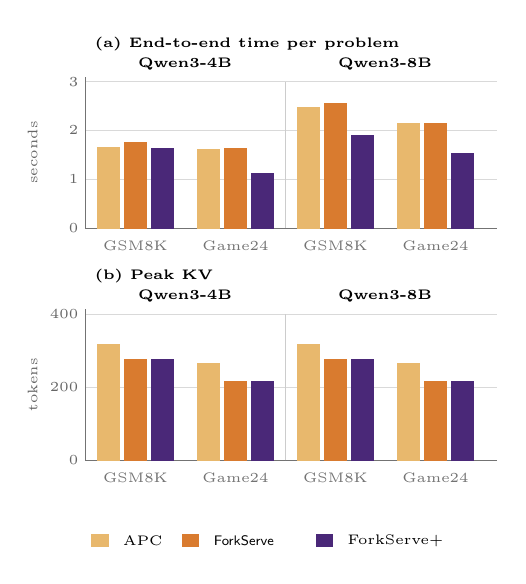
\begin{tikzpicture}[
  font=\scriptsize\sffamily,
  bar/.style={draw=black!55, line width=0.2pt},
  ax/.style={black!55, line width=0.35pt},
  grid/.style={black!15, line width=0.25pt},
  tick/.style={font=\tiny, text=black!60, inner sep=0pt},
  val/.style={font=\tiny, inner sep=0.2pt},
  wl/.style={font=\tiny, text=black!55, inner sep=0pt},
]
\definecolor{APC}{HTML}{E8B86D}
\definecolor{FS}{HTML}{D97B2F}
\definecolor{FSp}{HTML}{4A2878}

% (a) end-to-end seconds per problem. y = 0.38 + 0.62 * seconds. Axis 0--3 s.
\begin{scope}[shift={(0,2.95)}]
  \node[font=\tiny\bfseries, anchor=west] at (0.62,2.72) {(a) End-to-end time per problem};
  \draw[grid] (0.62,0.38) -- (5.85,0.38);
  \draw[grid] (0.62,1.00) -- (5.85,1.00);
  \draw[grid] (0.62,1.62) -- (5.85,1.62);
  \draw[grid] (0.62,2.24) -- (5.85,2.24);
  \draw[ax] (0.62,0.38) -- (5.85,0.38);
  \draw[ax] (0.62,0.38) -- (0.62,2.30);
  \node[tick, anchor=east] at (0.54,0.38) {0};
  \node[tick, anchor=east] at (0.54,1.00) {1};
  \node[tick, anchor=east] at (0.54,1.62) {2};
  \node[tick, anchor=east] at (0.54,2.24) {3};
  \node[tick, rotate=90, anchor=south] at (0.02,1.34) {seconds};
  \node[font=\tiny\bfseries] at (1.89,2.46) {Qwen3-4B};
  \node[font=\tiny\bfseries] at (4.43,2.46) {Qwen3-8B};
  \draw[black!20] (3.16,0.38) -- (3.16,2.24);
  % Qwen3-4B GSM8K: 1.66, 1.76, 1.63 s
  \fill[bar, APC] (0.78,0.38) rectangle (1.06,1.407);
  \fill[bar, FS]  (1.12,0.38) rectangle (1.40,1.474);
  \fill[bar, FSp] (1.46,0.38) rectangle (1.74,1.389);
  \node[wl] at (1.26,0.16) {GSM8K};
  % Qwen3-4B Game24: 1.61, 1.64, 1.13 s
  \fill[bar, APC] (2.05,0.38) rectangle (2.33,1.379);
  \fill[bar, FS]  (2.39,0.38) rectangle (2.67,1.396);
  \fill[bar, FSp] (2.73,0.38) rectangle (3.01,1.079);
  \node[wl] at (2.53,0.16) {Game24};
  % Qwen3-8B GSM8K: 2.48, 2.56, 1.91 s
  \fill[bar, APC] (3.32,0.38) rectangle (3.60,1.916);
  \fill[bar, FS]  (3.66,0.38) rectangle (3.94,1.968);
  \fill[bar, FSp] (4.00,0.38) rectangle (4.28,1.563);
  \node[wl] at (3.80,0.16) {GSM8K};
  % Qwen3-8B Game24: 2.15, 2.15, 1.52 s
  \fill[bar, APC] (4.59,0.38) rectangle (4.87,1.713);
  \fill[bar, FS]  (4.93,0.38) rectangle (5.21,1.716);
  \fill[bar, FSp] (5.27,0.38) rectangle (5.55,1.324);
  \node[wl] at (5.07,0.16) {Game24};
\end{scope}

% (b) peak KV. y = 0.38 + 0.00465 * tokens. Axis 0--400.
\begin{scope}[shift={(0,0)}]
  \node[font=\tiny\bfseries, anchor=west] at (0.62,2.72) {(b) Peak KV};
  \draw[grid] (0.62,0.38) -- (5.85,0.38);
  \draw[grid] (0.62,1.31) -- (5.85,1.31);
  \draw[grid] (0.62,2.24) -- (5.85,2.24);
  \draw[ax] (0.62,0.38) -- (5.85,0.38);
  \draw[ax] (0.62,0.38) -- (0.62,2.30);
  \node[tick, anchor=east] at (0.54,0.38) {0};
  \node[tick, anchor=east] at (0.54,1.31) {200};
  \node[tick, anchor=east] at (0.54,2.24) {400};
  \node[tick, rotate=90, anchor=south] at (0.02,1.34) {tokens};
  \node[font=\tiny\bfseries] at (1.89,2.46) {Qwen3-4B};
  \node[font=\tiny\bfseries] at (4.43,2.46) {Qwen3-8B};
  \draw[black!20] (3.16,0.38) -- (3.16,2.24);
  % GSM8K, both models: 318, 275, 275 tokens
  \fill[bar, APC] (0.78,0.38) rectangle (1.06,1.859);
  \fill[bar, FS]  (1.12,0.38) rectangle (1.40,1.659);
  \fill[bar, FSp] (1.46,0.38) rectangle (1.74,1.659);
  \node[wl] at (1.26,0.16) {GSM8K};
  % Game24, both models: 265, 216, 216 tokens
  \fill[bar, APC] (2.05,0.38) rectangle (2.33,1.612);
  \fill[bar, FS]  (2.39,0.38) rectangle (2.67,1.384);
  \fill[bar, FSp] (2.73,0.38) rectangle (3.01,1.384);
  \node[wl] at (2.53,0.16) {Game24};
  \fill[bar, APC] (3.32,0.38) rectangle (3.60,1.859);
  \fill[bar, FS]  (3.66,0.38) rectangle (3.94,1.659);
  \fill[bar, FSp] (4.00,0.38) rectangle (4.28,1.659);
  \node[wl] at (3.80,0.16) {GSM8K};
  \fill[bar, APC] (4.59,0.38) rectangle (4.87,1.612);
  \fill[bar, FS]  (4.93,0.38) rectangle (5.21,1.384);
  \fill[bar, FSp] (5.27,0.38) rectangle (5.55,1.384);
  \node[wl] at (5.07,0.16) {Game24};
\end{scope}

\fill[APC] (0.70,-0.72) rectangle (0.92,-0.56);
\node[font=\tiny, anchor=west] at (0.98,-0.64) {APC};
\fill[FS] (1.85,-0.72) rectangle (2.07,-0.56);
\node[font=\tiny, anchor=west] at (2.13,-0.64) {\sys};
\fill[FSp] (3.55,-0.72) rectangle (3.77,-0.56);
\node[font=\tiny, anchor=west] at (3.83,-0.64) {ForkServe+};
\end{tikzpicture}
}
\caption{\textbf{Three-turn ToT} on Qwen3-4B and Qwen3-8B ($n{=}16$, $\mathrm{tp}{=}2$, one problem per generate).
(a)~End-to-end seconds per problem; a shorter bar is faster.
(b)~Peak KV tokens.
\sys stays with APC on latency and stores the spine ($0.86\times$ APC on GSM8K, $0.82\times$ on Game24).
ForkServe+ is faster because it prefills one of four residuals.}
% and stops on a finished answer. (answer stop; do not describe it)
\label{fig:eval-mt}
\end{figure}

\paragraph{Depth keeps one spine.}
\Cref{tab:mt,fig:eval-mt} are GSM8K and Game24 under that schedule.
Peak KV is $275$ against APC $318$ on GSM8K ($0.86\times$) and $216$ against $265$ on Game24 ($0.82\times$), on both models.
\sys stays within $6\%$ of APC end-to-end ($1.00$--$1.06\times$).
Across $16$ problems, three turns, and four agents, the expand issues $192$ residuals.
ForkServe+ prefills $48$ of them and withholds the other $144$ before they reach the GPU.

\begin{table}[t]
\centering
\caption{Expand versus decode, milliseconds per problem.
Expand is the prefill of the $k$ residuals across three turns.
On APC that timer also includes the two $32$-token step decodes; \sys and ForkServe+ charge those steps to decode.
Speedup in \Cref{fig:eval-mt-split} is APC expand time over the other system.
Shortest time in each trio in green.}
\label{tab:mt-split}
\scriptsize
\setlength{\tabcolsep}{2.4pt}
\setlength{\aboverulesep}{0.35pt}
\setlength{\belowrulesep}{0.35pt}
\begin{tabular}{lrrrrrr}
\rowcolor{tblhead}
\toprule
 & \multicolumn{3}{c}{Expand (ms)} & \multicolumn{3}{c}{Decode (ms)} \\
\cmidrule(lr){2-4}\cmidrule(lr){5-7}
 & APC & FS & FS+ & APC & FS & FS+ \\
\midrule
4B GSM8K & $429$ & $83$ & \win{$55$} & \win{$1215$} & $1680$ & $1572$ \\
\rowcolor{tblalt}
4B Game24 & $435$ & $87$ & \win{$53$} & $1166$ & $1552$ & \win{$1074$} \\
8B GSM8K & $597$ & $94$ & \win{$58$} & $1867$ & $2468$ & \win{$1848$} \\
\rowcolor{tblalt}
8B Game24 & $598$ & $94$ & \win{$56$} & $1538$ & $2060$ & \win{$1466$} \\
\bottomrule
\end{tabular}
\end{table}

\begin{figure}[t]
\centering
\resizebox{\columnwidth}{!}{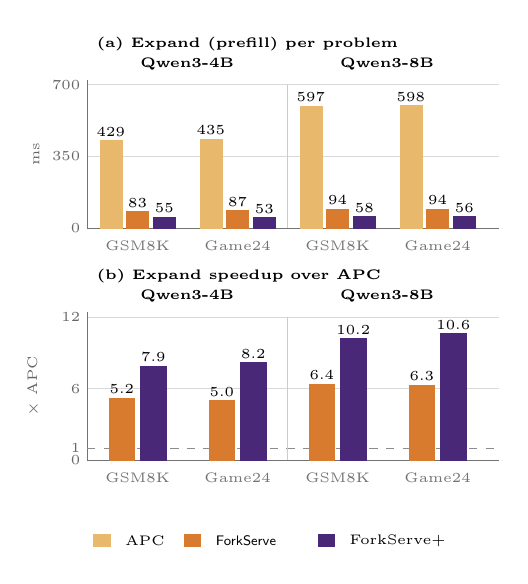
\begin{tikzpicture}[
  font=\scriptsize\sffamily,
  bar/.style={draw=black!55, line width=0.2pt},
  ax/.style={black!55, line width=0.35pt},
  grid/.style={black!15, line width=0.25pt},
  tick/.style={font=\tiny, text=black!60, inner sep=0pt},
  val/.style={font=\tiny, inner sep=0.2pt},
  wl/.style={font=\tiny, text=black!55, inner sep=0pt},
]
\definecolor{APC}{HTML}{E8B86D}
\definecolor{FS}{HTML}{D97B2F}
\definecolor{FSp}{HTML}{4A2878}

% (a) expand ms/problem. y = 0.38 + 0.0026 * ms. Axis 0--700 ms.
\begin{scope}[shift={(0,2.95)}]
  \node[font=\tiny\bfseries, anchor=west] at (0.62,2.72) {(a) Expand (prefill) per problem};
  \draw[grid] (0.62,0.38) -- (5.85,0.38);
  \draw[grid] (0.62,1.29) -- (5.85,1.29);
  \draw[grid] (0.62,2.20) -- (5.85,2.20);
  \draw[ax] (0.62,0.38) -- (5.85,0.38);
  \draw[ax] (0.62,0.38) -- (0.62,2.26);
  \node[tick, anchor=east] at (0.54,0.38) {0};
  \node[tick, anchor=east] at (0.54,1.29) {350};
  \node[tick, anchor=east] at (0.54,2.20) {700};
  \node[tick, rotate=90, anchor=south] at (0.02,1.32) {ms};
  \node[font=\tiny\bfseries] at (1.89,2.46) {Qwen3-4B};
  \node[font=\tiny\bfseries] at (4.43,2.46) {Qwen3-8B};
  \draw[black!20] (3.16,0.38) -- (3.16,2.20);
  % 4B GSM8K: 429, 83, 55
  \fill[bar, APC] (0.78,0.38) rectangle (1.06,1.495);
  \fill[bar, FS]  (1.12,0.38) rectangle (1.40,0.596);
  \fill[bar, FSp] (1.46,0.38) rectangle (1.74,0.523);
  \node[val] at (0.92,1.60) {429};
  \node[val] at (1.26,0.70) {83};
  \node[val] at (1.60,0.63) {55};
  \node[wl] at (1.26,0.16) {GSM8K};
  % 4B Game24: 435, 87, 53
  \fill[bar, APC] (2.05,0.38) rectangle (2.33,1.511);
  \fill[bar, FS]  (2.39,0.38) rectangle (2.67,0.606);
  \fill[bar, FSp] (2.73,0.38) rectangle (3.01,0.518);
  \node[val] at (2.19,1.62) {435};
  \node[val] at (2.53,0.71) {87};
  \node[val] at (2.87,0.62) {53};
  \node[wl] at (2.53,0.16) {Game24};
  % 8B GSM8K: 597, 94, 58
  \fill[bar, APC] (3.32,0.38) rectangle (3.60,1.932);
  \fill[bar, FS]  (3.66,0.38) rectangle (3.94,0.624);
  \fill[bar, FSp] (4.00,0.38) rectangle (4.28,0.531);
  \node[val] at (3.46,2.04) {597};
  \node[val] at (3.80,0.73) {94};
  \node[val] at (4.14,0.64) {58};
  \node[wl] at (3.80,0.16) {GSM8K};
  % 8B Game24: 598, 94, 56
  \fill[bar, APC] (4.59,0.38) rectangle (4.87,1.935);
  \fill[bar, FS]  (4.93,0.38) rectangle (5.21,0.624);
  \fill[bar, FSp] (5.27,0.38) rectangle (5.55,0.526);
  \node[val] at (4.73,2.04) {598};
  \node[val] at (5.07,0.73) {94};
  \node[val] at (5.41,0.63) {56};
  \node[wl] at (5.07,0.16) {Game24};
\end{scope}

% (b) expand speedup vs APC. y = 0.38 + 0.15167 * ratio. Axis 0--12x.
\begin{scope}[shift={(0,0)}]
  \node[font=\tiny\bfseries, anchor=west] at (0.62,2.72) {(b) Expand speedup over APC};
  \draw[grid] (0.62,0.38) -- (5.85,0.38);
  \draw[grid] (0.62,1.29) -- (5.85,1.29);
  \draw[grid] (0.62,2.20) -- (5.85,2.20);
  \draw[ax] (0.62,0.38) -- (5.85,0.38);
  \draw[ax] (0.62,0.38) -- (0.62,2.26);
  \draw[black!45, dashed] (0.62,0.532) -- (5.85,0.532);
  \node[tick, anchor=east] at (0.54,0.38) {0};
  \node[tick, anchor=east] at (0.54,0.532) {1};
  \node[tick, anchor=east] at (0.54,1.29) {6};
  \node[tick, anchor=east] at (0.54,2.20) {12};
  \node[tick, rotate=90, anchor=south] at (0.02,1.32) {$\times$ APC};
  \node[font=\tiny\bfseries] at (1.89,2.46) {Qwen3-4B};
  \node[font=\tiny\bfseries] at (4.43,2.46) {Qwen3-8B};
  \draw[black!20] (3.16,0.38) -- (3.16,2.20);
  % 5.2, 7.9
  \fill[bar, FS]  (0.90,0.38) rectangle (1.22,1.169);
  \fill[bar, FSp] (1.30,0.38) rectangle (1.62,1.578);
  \node[val] at (1.06,1.28) {5.2};
  \node[val] at (1.46,1.69) {7.9};
  \node[wl] at (1.26,0.16) {GSM8K};
  % 5.0, 8.2
  \fill[bar, FS]  (2.17,0.38) rectangle (2.49,1.138);
  \fill[bar, FSp] (2.57,0.38) rectangle (2.89,1.624);
  \node[val] at (2.33,1.25) {5.0};
  \node[val] at (2.73,1.73) {8.2};
  \node[wl] at (2.53,0.16) {Game24};
  % 6.4, 10.2
  \fill[bar, FS]  (3.44,0.38) rectangle (3.76,1.351);
  \fill[bar, FSp] (3.84,0.38) rectangle (4.16,1.927);
  \node[val] at (3.60,1.46) {6.4};
  \node[val] at (4.00,2.04) {10.2};
  \node[wl] at (3.80,0.16) {GSM8K};
  % 6.3, 10.6
  \fill[bar, FS]  (4.71,0.38) rectangle (5.03,1.336);
  \fill[bar, FSp] (5.11,0.38) rectangle (5.43,1.988);
  \node[val] at (4.87,1.45) {6.3};
  \node[val] at (5.27,2.10) {10.6};
  \node[wl] at (5.07,0.16) {Game24};
\end{scope}

\fill[APC] (0.70,-0.72) rectangle (0.92,-0.56);
\node[font=\tiny, anchor=west] at (0.98,-0.64) {APC};
\fill[FS] (1.85,-0.72) rectangle (2.07,-0.56);
\node[font=\tiny, anchor=west] at (2.13,-0.64) {\sys};
\fill[FSp] (3.55,-0.72) rectangle (3.77,-0.56);
\node[font=\tiny, anchor=west] at (3.83,-0.64) {ForkServe+};
\end{tikzpicture}
}
\caption{\textbf{Expand versus APC} on the same four runs as \Cref{tab:mt-split}.
(a)~Expand milliseconds per problem.
(b)~Speedup of that expand over APC. The dashed line is $1\times$.
\sys is $5.0$--$6.4\times$ and ForkServe+ is $7.9$--$10.6\times$.
Decode in \Cref{tab:mt-split} does not repeat that ratio: the step decodes sit in the \sys decode column, so \sys end-to-end stays with APC.}
\label{fig:eval-mt-split}
\end{figure}

\Cref{tab:mt-split,fig:eval-mt-split} separate that expand from the winner decode.
The expand speedup is $5.0$--$6.4\times$ for \sys and $7.9$--$10.6\times$ for ForkServe+.
Decode does not match it.
\sys decode is slower than APC because the two step decodes are timed there, which is why end-to-end stays at $1.00$--$1.06\times$.
% Answer stop, not for the paper. It moves end-to-end only when it shortens
% the trace. Qwen3-4B GSM8K stays at 0.98x (208 vs 214 tokens; 1.63s vs 1.66s).
% Where it cuts the answer, end-to-end is 0.70--0.77x: Qwen3-4B Game24 1.13s
% vs 1.61s (121 vs 205 tokens), Qwen3-8B GSM8K 1.91s vs 2.48s (155 vs 225),
% Qwen3-8B Game24 1.52s vs 2.15s (109 vs 184).
GSM8K accuracy matches APC on Qwen3-4B ($15/16$ on the same problems) and is one problem lower on Qwen3-8B ($15/16$ vs.\ $16/16$).
On Game24, \sys solves two more problems than APC on Qwen3-4B ($8/16$ vs.\ $6/16$) and the same nine on Qwen3-8B; ForkServe+ solves $9/16$ and $10/16$.

\subsection{Cross-model forest}
\label{sec:eval-multi}

\paragraph{Setup.}
Same four systems, $n{=}40$, $D{=}512$, $\mathrm{tp}{=}2$ and $4$, on Qwen3-4B, Qwen2.5-Math-1.5B, Qwen3-14B, Llama-3-8B-Instruct, Mistral-7B-Instruct, and DeepSeek-R1-Distill-Llama-8B.

\iffalse
\begin{table}[t]
\centering
\caption{Cross-model forest, $n{=}40$, $\mathrm{tp}{=}2$ (peak KV unchanged at $\mathrm{tp}{=}4$).
APC decode tokens are $nD{=}20480$.
Game24 peaks use the same $k{=}4$ ToT.
R1 ForkServe+ accuracy is the last-line stop ($n{=}32$, $18/32$); the $n{=}40$ bare-marker run is omitted.
Best storage in green.}
\label{tab:multi}
\scriptsize
\setlength{\tabcolsep}{2.2pt}
\setlength{\aboverulesep}{0.35pt}
\setlength{\belowrulesep}{0.35pt}
\begin{tabular}{lrrrrrr}
\rowcolor{tblhead}
\toprule
 & 4B & 1.5B & 14B & L8B & M7B & R1 \\
\midrule
Rec.\ GSM8K & $4464$ & $4464$ & $4464$ & $4452$ & $4668$ & $4036$ \\
\rowcolor{tblalt}
APC GSM8K & $1512$ & $1512$ & $1512$ & $1509$ & $1569$ & $1405$ \\
FS GSM8K & \win{$1112$} & \win{$1112$} & \win{$1112$} & \win{$1109$} & \win{$1169$} & \win{$1005$} \\
\rowcolor{tblalt}
FS+ GSM8K & \win{$1112$} & \win{$1112$} & \win{$1112$} & \win{$1109$} & \win{$1169$} & \win{$1005$} \\
GSM8K / APC & \win{$0.74$} & \win{$0.74$} & \win{$0.74$} & \win{$0.73$} & \win{$0.75$} & \win{$0.72$} \\
\rowcolor{tblalt}
GSM8K / rec. & \win{$0.25$} & \win{$0.25$} & \win{$0.25$} & \win{$0.25$} & \win{$0.25$} & \win{$0.25$} \\
Rec.\ Game24 & $3060$ & $3060$ & $3060$ & $2952$ & $3100$ & $2536$ \\
\rowcolor{tblalt}
APC Game24 & $1287$ & $1287$ & $1287$ & $1248$ & $1351$ & $1144$ \\
FS Game24 & \win{$791$} & \win{$791$} & \win{$791$} & \win{$760$} & \win{$783$} & \win{$656$} \\
\rowcolor{tblalt}
FS+ Game24 & \win{$791$} & \win{$791$} & \win{$791$} & \win{$760$} & \win{$783$} & \win{$656$} \\
Game24 / APC & \win{$0.61$} & \win{$0.61$} & \win{$0.61$} & \win{$0.61$} & \win{$0.58$} & \win{$0.57$} \\
\rowcolor{tblalt}
APC acc. & $0.925$ & $0.225$ & $0.850$ & $0.625$ & $0.500$ & $0.650$ \\
FS acc. & $0.875$ & $0.275$ & $0.825$ & $0.675$ & $0.475$ & $0.650$ \\
\rowcolor{tblalt}
FS+ acc. & $0.550$ & $0.275$ & $0.725$ & $0.675$ & $0.350$ & $0.562$ \\
\bottomrule
\end{tabular}
\end{table}
\fi

\begin{figure}[t]
\centering
\resizebox{\columnwidth}{!}{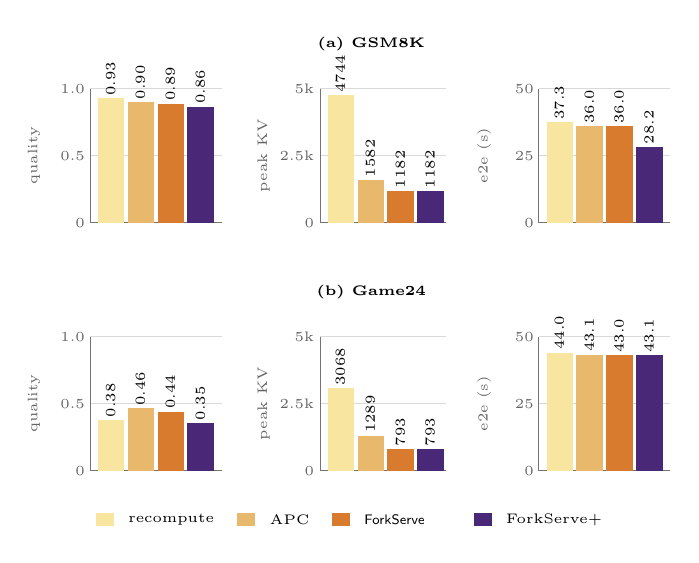
\begin{tikzpicture}[
  font=\scriptsize\sffamily,
  bar/.style={draw=black!55, line width=0.2pt},
  ax/.style={black!55, line width=0.35pt},
  grid/.style={black!15, line width=0.25pt},
  tick/.style={font=\tiny, text=black!60, inner sep=0pt},
  val/.style={font=\tiny, inner sep=0.3pt},
]
\definecolor{Rec}{HTML}{F8E6A0}
\definecolor{APC}{HTML}{E8B86D}
\definecolor{FS}{HTML}{D97B2F}
\definecolor{FSp}{HTML}{4A2878}

% --- (a) GSM8K, y shift 3.15 ---
\begin{scope}[shift={(0,3.15)}]
  \node[font=\tiny\bfseries] at (4.05,2.55) {(a) GSM8K};
  % quality, ymax 1.0
  \begin{scope}[shift={(0,0)}]
    \draw[grid] (0.48,0.28) -- (2.15,0.28) (0.48,1.13) -- (2.15,1.13) (0.48,1.98) -- (2.15,1.98);
    \draw[ax] (0.48,0.28) -- (2.15,0.28) (0.48,0.28) -- (0.48,1.98);
    \node[tick, anchor=east] at (0.42,0.28) {0};
    \node[tick, anchor=east] at (0.42,1.13) {0.5};
    \node[tick, anchor=east] at (0.42,1.98) {1.0};
    \node[tick, rotate=90, anchor=south] at (-0.15,1.13) {quality};
    \fill[bar, Rec] (0.58,0.28) rectangle (0.90,1.853);
    \fill[bar, APC] (0.96,0.28) rectangle (1.28,1.810);
    \fill[bar, FS]  (1.34,0.28) rectangle (1.66,1.788);
    \fill[bar, FSp] (1.72,0.28) rectangle (2.04,1.747);
    \node[val, rotate=90, anchor=west] at (0.74,1.87) {0.93};
    \node[val, rotate=90, anchor=west] at (1.12,1.83) {0.90};
    \node[val, rotate=90, anchor=west] at (1.50,1.81) {0.89};
    \node[val, rotate=90, anchor=west] at (1.88,1.77) {0.86};
  \end{scope}
  % peak KV, ymax 5k
  \begin{scope}[shift={(2.85,0)}]
    \draw[grid] (0.55,0.28) -- (2.15,0.28) (0.55,1.13) -- (2.15,1.13) (0.55,1.98) -- (2.15,1.98);
    \draw[ax] (0.55,0.28) -- (2.15,0.28) (0.55,0.28) -- (0.55,1.98);
    \node[tick, anchor=east] at (0.48,0.28) {0};
    \node[tick, anchor=east] at (0.48,1.13) {2.5k};
    \node[tick, anchor=east] at (0.48,1.98) {5k};
    \node[tick, rotate=90, anchor=south] at (-0.08,1.13) {peak KV};
    \fill[bar, Rec] (0.65,0.28) rectangle (0.97,1.893);
    \fill[bar, APC] (1.03,0.28) rectangle (1.35,0.818);
    \fill[bar, FS]  (1.41,0.28) rectangle (1.73,0.682);
    \fill[bar, FSp] (1.79,0.28) rectangle (2.11,0.682);
    \node[val, rotate=90, anchor=west] at (0.81,1.91) {4744};
    \node[val, rotate=90, anchor=west] at (1.19,0.84) {1582};
    \node[val, rotate=90, anchor=west] at (1.57,0.70) {1182};
    \node[val, rotate=90, anchor=west] at (1.95,0.70) {1182};
  \end{scope}
  % e2e seconds, ymax 50, shorter is faster
  \begin{scope}[shift={(5.70,0)}]
    \draw[grid] (0.48,0.28) -- (2.15,0.28) (0.48,1.13) -- (2.15,1.13) (0.48,1.98) -- (2.15,1.98);
    \draw[ax] (0.48,0.28) -- (2.15,0.28) (0.48,0.28) -- (0.48,1.98);
    \node[tick, anchor=east] at (0.42,0.28) {0};
    \node[tick, anchor=east] at (0.42,1.13) {25};
    \node[tick, anchor=east] at (0.42,1.98) {50};
    \node[tick, rotate=90, anchor=south] at (-0.12,1.13) {e2e (s)};
    \fill[bar, Rec] (0.58,0.28) rectangle (0.90,1.550);
    \fill[bar, APC] (0.96,0.28) rectangle (1.28,1.504);
    \fill[bar, FS]  (1.34,0.28) rectangle (1.66,1.505);
    \fill[bar, FSp] (1.72,0.28) rectangle (2.04,1.239);
    \node[val, rotate=90, anchor=west] at (0.74,1.57) {37.3};
    \node[val, rotate=90, anchor=west] at (1.12,1.52) {36.0};
    \node[val, rotate=90, anchor=west] at (1.50,1.52) {36.0};
    \node[val, rotate=90, anchor=west] at (1.88,1.26) {28.2};
  \end{scope}
\end{scope}

% --- (b) Game24 ---
\begin{scope}[shift={(0,0)}]
  \node[font=\tiny\bfseries] at (4.05,2.55) {(b) Game24};
  \begin{scope}[shift={(0,0)}]
    \draw[grid] (0.48,0.28) -- (2.15,0.28) (0.48,1.13) -- (2.15,1.13) (0.48,1.98) -- (2.15,1.98);
    \draw[ax] (0.48,0.28) -- (2.15,0.28) (0.48,0.28) -- (0.48,1.98);
    \node[tick, anchor=east] at (0.42,0.28) {0};
    \node[tick, anchor=east] at (0.42,1.13) {0.5};
    \node[tick, anchor=east] at (0.42,1.98) {1.0};
    \node[tick, rotate=90, anchor=south] at (-0.15,1.13) {quality};
    \fill[bar, Rec] (0.58,0.28) rectangle (0.90,0.917);
    \fill[bar, APC] (0.96,0.28) rectangle (1.28,1.067);
    \fill[bar, FS]  (1.34,0.28) rectangle (1.66,1.025);
    \fill[bar, FSp] (1.72,0.28) rectangle (2.04,0.875);
    \node[val, rotate=90, anchor=west] at (0.74,0.94) {0.38};
    \node[val, rotate=90, anchor=west] at (1.12,1.09) {0.46};
    \node[val, rotate=90, anchor=west] at (1.50,1.05) {0.44};
    \node[val, rotate=90, anchor=west] at (1.88,0.90) {0.35};
  \end{scope}
  \begin{scope}[shift={(2.85,0)}]
    \draw[grid] (0.55,0.28) -- (2.15,0.28) (0.55,1.13) -- (2.15,1.13) (0.55,1.98) -- (2.15,1.98);
    \draw[ax] (0.55,0.28) -- (2.15,0.28) (0.55,0.28) -- (0.55,1.98);
    \node[tick, anchor=east] at (0.48,0.28) {0};
    \node[tick, anchor=east] at (0.48,1.13) {2.5k};
    \node[tick, anchor=east] at (0.48,1.98) {5k};
    \node[tick, rotate=90, anchor=south] at (-0.08,1.13) {peak KV};
    \fill[bar, Rec] (0.65,0.28) rectangle (0.97,1.323);
    \fill[bar, APC] (1.03,0.28) rectangle (1.35,0.718);
    \fill[bar, FS]  (1.41,0.28) rectangle (1.73,0.550);
    \fill[bar, FSp] (1.79,0.28) rectangle (2.11,0.550);
    \node[val, rotate=90, anchor=west] at (0.81,1.34) {3068};
    \node[val, rotate=90, anchor=west] at (1.19,0.74) {1289};
    \node[val, rotate=90, anchor=west] at (1.57,0.57) {793};
    \node[val, rotate=90, anchor=west] at (1.95,0.57) {793};
  \end{scope}
  \begin{scope}[shift={(5.70,0)}]
    \draw[grid] (0.48,0.28) -- (2.15,0.28) (0.48,1.13) -- (2.15,1.13) (0.48,1.98) -- (2.15,1.98);
    \draw[ax] (0.48,0.28) -- (2.15,0.28) (0.48,0.28) -- (0.48,1.98);
    \node[tick, anchor=east] at (0.42,0.28) {0};
    \node[tick, anchor=east] at (0.42,1.13) {25};
    \node[tick, anchor=east] at (0.42,1.98) {50};
    \node[tick, rotate=90, anchor=south] at (-0.12,1.13) {e2e (s)};
    \fill[bar, Rec] (0.58,0.28) rectangle (0.90,1.775);
    \fill[bar, APC] (0.96,0.28) rectangle (1.28,1.747);
    \fill[bar, FS]  (1.34,0.28) rectangle (1.66,1.741);
    \fill[bar, FSp] (1.72,0.28) rectangle (2.04,1.744);
    \node[val, rotate=90, anchor=west] at (0.74,1.80) {44.0};
    \node[val, rotate=90, anchor=west] at (1.12,1.77) {43.1};
    \node[val, rotate=90, anchor=west] at (1.50,1.76) {43.0};
    \node[val, rotate=90, anchor=west] at (1.88,1.76) {43.1};
  \end{scope}
\end{scope}

\fill[Rec] (0.55,-0.42) rectangle (0.78,-0.26);
\node[font=\tiny, anchor=west] at (0.84,-0.34) {recompute};
\fill[APC] (2.35,-0.42) rectangle (2.58,-0.26);
\node[font=\tiny, anchor=west] at (2.64,-0.34) {APC};
\fill[FS] (3.55,-0.42) rectangle (3.78,-0.26);
\node[font=\tiny, anchor=west] at (3.84,-0.34) {\sys};
\fill[FSp] (5.35,-0.42) rectangle (5.58,-0.26);
\node[font=\tiny, anchor=west] at (5.64,-0.34) {ForkServe+};
\end{tikzpicture}
}
\caption{\textbf{Four systems on Qwen3-8B} ($n{=}80$, $\mathrm{tp}{=}2$, $D{=}512$).
Each panel has its own axis. Quality is higher-better; peak KV and end-to-end time are the measured values, so a shorter bar is better.
(a)~GSM8K. (b)~Game24.
\Cref{fig:eval-radar} shows that \sys and ForkServe+ lower peak KV below APC on both workloads ($0.75\times$ on GSM8K, $0.62\times$ on Game24) while GSM8K quality stays with APC, and that ForkServe+ also lowers GSM8K end-to-end time from $36.0$\,s to $28.2$\,s.}
\label{fig:eval-radar}
\end{figure}

\paragraph{Peak occupancy.}
APC retains the shared trunk and the union of the residuals, which is the copy-on-write term $M_{\mathrm{APC}}=M_{\mathrm{CoW}}=b\bigl(L+\sum_i\ell_i\bigr)$ from \eqref{eq:mem}. The tree retains only the committed spine $M_{\mathrm{spine}}=b(L+\ell_\star)$.
The ratio of these two terms cancels $b$ and equals $(L+\ell_\star)/(L+\sum_i\ell_i)$, so it depends on $k$ and the lengths $(L,\ell_\star)$ rather than on the weights or the tensor width.
When the residuals have similar length, the ratio simplifies to $(L+\ell)/(L+k\ell)$ and decreases as $L/\ell$ decreases.
\Cref{fig:eval-multi} shows this pattern: a long trunk on GSM8K gives $0.72$--$0.75$, and a shorter trunk on Game24 gives $0.57$--$0.61$.
\Cref{fig:eval-radar} repeats the comparison at $n{=}80$ with recompute and ForkServe+ on separate axes.
Relative to recompute, which stores the cloned occupancy $M_{\mathrm{clone}}$, the spine is $0.25\times$.
ForkServe+ matches that ratio.
Accuracy remains at the APC level, which indicates that the lower peak is a storage effect on the same committed answer.
\Cref{fig:eval-hist} shows the per-item decode-length distribution on GSM8K and Game24.
% DeepSeek-R1 ForkServe+ on the last-line slice is $18/32$ against APC $16/32$ on the same $32$ items.

\begin{figure*}[t]
\centering
\resizebox{\textwidth}{!}{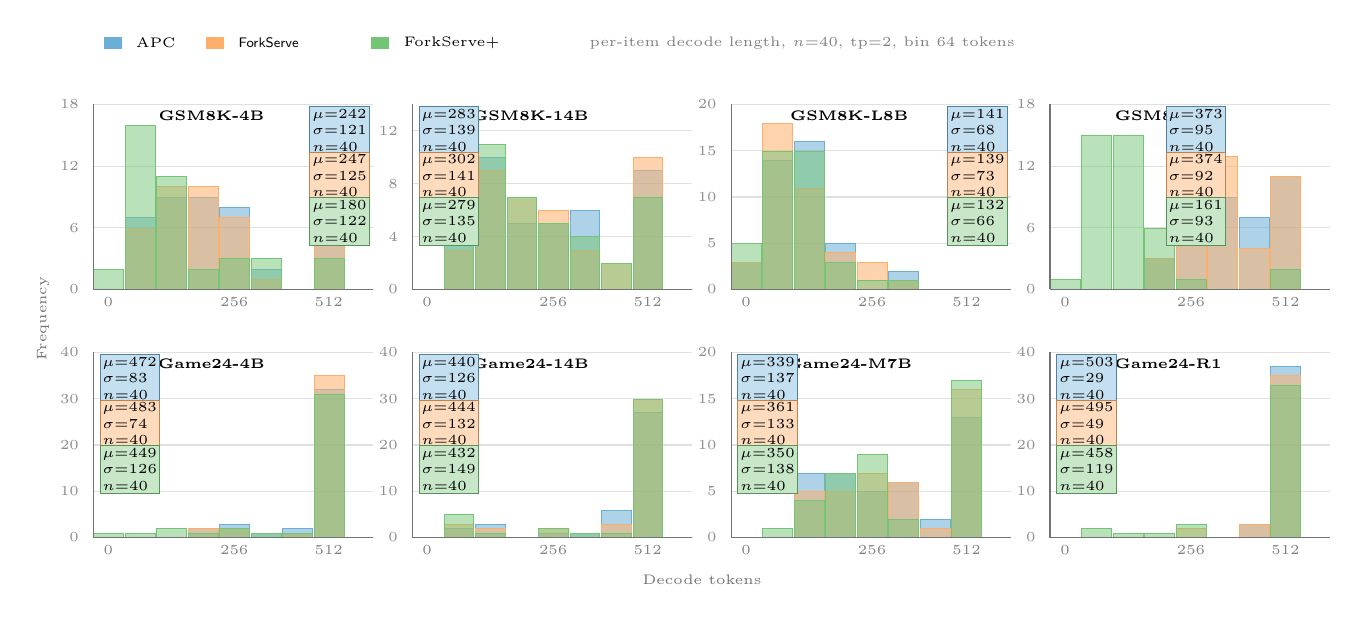
\begin{tikzpicture}[
  font=\scriptsize\sffamily,
  bar/.style={draw=black!50, line width=0.12pt},
]
\definecolor{APC}{HTML}{6BAED6}
\definecolor{FS}{HTML}{FDAE6B}
\definecolor{FSp}{HTML}{74C476}

\fill[APC] (0.55,6.62) rectangle (0.78,6.78);
\node[font=\tiny, anchor=west] at (0.84,6.70) {APC};
\fill[FS] (1.85,6.62) rectangle (2.08,6.78);
\node[font=\tiny, anchor=west] at (2.14,6.70) {\sys};
\fill[FSp] (3.95,6.62) rectangle (4.18,6.78);
\node[font=\tiny, anchor=west] at (4.24,6.70) {ForkServe+};
\node[font=\tiny, text=black!50, anchor=west] at (6.6,6.70)
  {per-item decode length, $n{=}40$, $\mathrm{tp}{=}2$, bin $64$ tokens};

% --- GSM8K-4B ---
\begin{scope}[shift={(0.00,3.25)}]
  \node[font=\tiny\bfseries] at (1.92,2.53) {GSM8K-4B};
  \draw[black!12] (0.42,0.320) -- (3.97,0.320);
  \node[font=\tiny, text=black!45, anchor=east] at (0.36,0.320) {0};
  \draw[black!12] (0.42,1.103) -- (3.97,1.103);
  \node[font=\tiny, text=black!45, anchor=east] at (0.36,1.103) {6};
  \draw[black!12] (0.42,1.887) -- (3.97,1.887);
  \node[font=\tiny, text=black!45, anchor=east] at (0.36,1.887) {12};
  \draw[black!12] (0.42,2.670) -- (3.97,2.670);
  \node[font=\tiny, text=black!45, anchor=east] at (0.36,2.670) {18};
  \fill[bar, FSp, fill opacity=0.5] (0.420,0.32) rectangle (0.800,0.581);
  \fill[bar, APC, fill opacity=0.55] (0.820,0.32) rectangle (1.200,1.234);
  \fill[bar, FS, fill opacity=0.55] (0.820,0.32) rectangle (1.200,1.103);
  \fill[bar, FSp, fill opacity=0.5] (0.820,0.32) rectangle (1.200,2.409);
  \fill[bar, APC, fill opacity=0.55] (1.220,0.32) rectangle (1.600,1.495);
  \fill[bar, FS, fill opacity=0.55] (1.220,0.32) rectangle (1.600,1.626);
  \fill[bar, FSp, fill opacity=0.5] (1.220,0.32) rectangle (1.600,1.756);
  \fill[bar, APC, fill opacity=0.55] (1.620,0.32) rectangle (2.000,1.495);
  \fill[bar, FS, fill opacity=0.55] (1.620,0.32) rectangle (2.000,1.626);
  \fill[bar, FSp, fill opacity=0.5] (1.620,0.32) rectangle (2.000,0.581);
  \fill[bar, APC, fill opacity=0.55] (2.020,0.32) rectangle (2.400,1.364);
  \fill[bar, FS, fill opacity=0.55] (2.020,0.32) rectangle (2.400,1.234);
  \fill[bar, FSp, fill opacity=0.5] (2.020,0.32) rectangle (2.400,0.712);
  \fill[bar, APC, fill opacity=0.55] (2.420,0.32) rectangle (2.800,0.581);
  \fill[bar, FS, fill opacity=0.55] (2.420,0.32) rectangle (2.800,0.451);
  \fill[bar, FSp, fill opacity=0.5] (2.420,0.32) rectangle (2.800,0.712);
  \fill[bar, APC, fill opacity=0.55] (3.220,0.32) rectangle (3.600,0.973);
  \fill[bar, FS, fill opacity=0.55] (3.220,0.32) rectangle (3.600,1.103);
  \fill[bar, FSp, fill opacity=0.5] (3.220,0.32) rectangle (3.600,0.712);
  \draw[black!55] (0.42,0.32) -- (3.97,0.32);
  \draw[black!55] (0.42,0.32) -- (0.42,2.67);
  \node[font=\tiny, text=black!50] at (0.610,0.16) {0};
  \node[font=\tiny, text=black!50] at (2.210,0.16) {256};
  \node[font=\tiny, text=black!50] at (3.410,0.16) {512};
  \node[font=\tiny, inner sep=1.0pt, align=left, rectangle, fill=APC!40, draw=APC!75!black, line width=0.2pt, anchor=north east] at (3.93,2.65)
    {$\mu{=}242$\\$\sigma{=}121$\\$n{=}40$};
  \node[font=\tiny, inner sep=1.0pt, align=left, rectangle, fill=FS!45, draw=FS!75!black, line width=0.2pt, anchor=north east] at (3.93,2.07)
    {$\mu{=}247$\\$\sigma{=}125$\\$n{=}40$};
  \node[font=\tiny, inner sep=1.0pt, align=left, rectangle, fill=FSp!40, draw=FSp!75!black, line width=0.2pt, anchor=north east] at (3.93,1.49)
    {$\mu{=}180$\\$\sigma{=}122$\\$n{=}40$};
\end{scope}

% --- GSM8K-14B ---
\begin{scope}[shift={(4.05,3.25)}]
  \node[font=\tiny\bfseries] at (1.92,2.53) {GSM8K-14B};
  \draw[black!12] (0.42,0.320) -- (3.97,0.320);
  \node[font=\tiny, text=black!45, anchor=east] at (0.36,0.320) {0};
  \draw[black!12] (0.42,0.991) -- (3.97,0.991);
  \node[font=\tiny, text=black!45, anchor=east] at (0.36,0.991) {4};
  \draw[black!12] (0.42,1.663) -- (3.97,1.663);
  \node[font=\tiny, text=black!45, anchor=east] at (0.36,1.663) {8};
  \draw[black!12] (0.42,2.334) -- (3.97,2.334);
  \node[font=\tiny, text=black!45, anchor=east] at (0.36,2.334) {12};
  \fill[bar, APC, fill opacity=0.55] (0.820,0.32) rectangle (1.200,1.159);
  \fill[bar, FS, fill opacity=0.55] (0.820,0.32) rectangle (1.200,0.824);
  \fill[bar, FSp, fill opacity=0.5] (0.820,0.32) rectangle (1.200,0.991);
  \fill[bar, APC, fill opacity=0.55] (1.220,0.32) rectangle (1.600,1.999);
  \fill[bar, FS, fill opacity=0.55] (1.220,0.32) rectangle (1.600,1.831);
  \fill[bar, FSp, fill opacity=0.5] (1.220,0.32) rectangle (1.600,2.166);
  \fill[bar, APC, fill opacity=0.55] (1.620,0.32) rectangle (2.000,1.159);
  \fill[bar, FS, fill opacity=0.55] (1.620,0.32) rectangle (2.000,1.495);
  \fill[bar, FSp, fill opacity=0.5] (1.620,0.32) rectangle (2.000,1.495);
  \fill[bar, APC, fill opacity=0.55] (2.020,0.32) rectangle (2.400,1.159);
  \fill[bar, FS, fill opacity=0.55] (2.020,0.32) rectangle (2.400,1.327);
  \fill[bar, FSp, fill opacity=0.5] (2.020,0.32) rectangle (2.400,1.159);
  \fill[bar, APC, fill opacity=0.55] (2.420,0.32) rectangle (2.800,1.327);
  \fill[bar, FS, fill opacity=0.55] (2.420,0.32) rectangle (2.800,0.824);
  \fill[bar, FSp, fill opacity=0.5] (2.420,0.32) rectangle (2.800,0.991);
  \fill[bar, FS, fill opacity=0.55] (2.820,0.32) rectangle (3.200,0.656);
  \fill[bar, FSp, fill opacity=0.5] (2.820,0.32) rectangle (3.200,0.656);
  \fill[bar, APC, fill opacity=0.55] (3.220,0.32) rectangle (3.600,1.831);
  \fill[bar, FS, fill opacity=0.55] (3.220,0.32) rectangle (3.600,1.999);
  \fill[bar, FSp, fill opacity=0.5] (3.220,0.32) rectangle (3.600,1.495);
  \draw[black!55] (0.42,0.32) -- (3.97,0.32);
  \draw[black!55] (0.42,0.32) -- (0.42,2.67);
  \node[font=\tiny, text=black!50] at (0.610,0.16) {0};
  \node[font=\tiny, text=black!50] at (2.210,0.16) {256};
  \node[font=\tiny, text=black!50] at (3.410,0.16) {512};
  \node[font=\tiny, inner sep=1.0pt, align=left, rectangle, fill=APC!40, draw=APC!75!black, line width=0.2pt, anchor=north west] at (0.50,2.65)
    {$\mu{=}283$\\$\sigma{=}139$\\$n{=}40$};
  \node[font=\tiny, inner sep=1.0pt, align=left, rectangle, fill=FS!45, draw=FS!75!black, line width=0.2pt, anchor=north west] at (0.50,2.07)
    {$\mu{=}302$\\$\sigma{=}141$\\$n{=}40$};
  \node[font=\tiny, inner sep=1.0pt, align=left, rectangle, fill=FSp!40, draw=FSp!75!black, line width=0.2pt, anchor=north west] at (0.50,1.49)
    {$\mu{=}279$\\$\sigma{=}135$\\$n{=}40$};
\end{scope}

% --- GSM8K-L8B ---
\begin{scope}[shift={(8.10,3.25)}]
  \node[font=\tiny\bfseries] at (1.92,2.53) {GSM8K-L8B};
  \draw[black!12] (0.42,0.320) -- (3.97,0.320);
  \node[font=\tiny, text=black!45, anchor=east] at (0.36,0.320) {0};
  \draw[black!12] (0.42,0.907) -- (3.97,0.907);
  \node[font=\tiny, text=black!45, anchor=east] at (0.36,0.907) {5};
  \draw[black!12] (0.42,1.495) -- (3.97,1.495);
  \node[font=\tiny, text=black!45, anchor=east] at (0.36,1.495) {10};
  \draw[black!12] (0.42,2.083) -- (3.97,2.083);
  \node[font=\tiny, text=black!45, anchor=east] at (0.36,2.083) {15};
  \draw[black!12] (0.42,2.670) -- (3.97,2.670);
  \node[font=\tiny, text=black!45, anchor=east] at (0.36,2.670) {20};
  \fill[bar, APC, fill opacity=0.55] (0.420,0.32) rectangle (0.800,0.672);
  \fill[bar, FS, fill opacity=0.55] (0.420,0.32) rectangle (0.800,0.672);
  \fill[bar, FSp, fill opacity=0.5] (0.420,0.32) rectangle (0.800,0.907);
  \fill[bar, APC, fill opacity=0.55] (0.820,0.32) rectangle (1.200,1.965);
  \fill[bar, FS, fill opacity=0.55] (0.820,0.32) rectangle (1.200,2.435);
  \fill[bar, FSp, fill opacity=0.5] (0.820,0.32) rectangle (1.200,2.083);
  \fill[bar, APC, fill opacity=0.55] (1.220,0.32) rectangle (1.600,2.200);
  \fill[bar, FS, fill opacity=0.55] (1.220,0.32) rectangle (1.600,1.613);
  \fill[bar, FSp, fill opacity=0.5] (1.220,0.32) rectangle (1.600,2.083);
  \fill[bar, APC, fill opacity=0.55] (1.620,0.32) rectangle (2.000,0.907);
  \fill[bar, FS, fill opacity=0.55] (1.620,0.32) rectangle (2.000,0.790);
  \fill[bar, FSp, fill opacity=0.5] (1.620,0.32) rectangle (2.000,0.672);
  \fill[bar, FS, fill opacity=0.55] (2.020,0.32) rectangle (2.400,0.672);
  \fill[bar, FSp, fill opacity=0.5] (2.020,0.32) rectangle (2.400,0.438);
  \fill[bar, APC, fill opacity=0.55] (2.420,0.32) rectangle (2.800,0.555);
  \fill[bar, FS, fill opacity=0.55] (2.420,0.32) rectangle (2.800,0.438);
  \fill[bar, FSp, fill opacity=0.5] (2.420,0.32) rectangle (2.800,0.438);
  \draw[black!55] (0.42,0.32) -- (3.97,0.32);
  \draw[black!55] (0.42,0.32) -- (0.42,2.67);
  \node[font=\tiny, text=black!50] at (0.610,0.16) {0};
  \node[font=\tiny, text=black!50] at (2.210,0.16) {256};
  \node[font=\tiny, text=black!50] at (3.410,0.16) {512};
  \node[font=\tiny, inner sep=1.0pt, align=left, rectangle, fill=APC!40, draw=APC!75!black, line width=0.2pt, anchor=north east] at (3.93,2.65)
    {$\mu{=}141$\\$\sigma{=}68$\\$n{=}40$};
  \node[font=\tiny, inner sep=1.0pt, align=left, rectangle, fill=FS!45, draw=FS!75!black, line width=0.2pt, anchor=north east] at (3.93,2.07)
    {$\mu{=}139$\\$\sigma{=}73$\\$n{=}40$};
  \node[font=\tiny, inner sep=1.0pt, align=left, rectangle, fill=FSp!40, draw=FSp!75!black, line width=0.2pt, anchor=north east] at (3.93,1.49)
    {$\mu{=}132$\\$\sigma{=}66$\\$n{=}40$};
\end{scope}

% --- GSM8K-R1 ---
\begin{scope}[shift={(12.15,3.25)}]
  \node[font=\tiny\bfseries] at (1.92,2.53) {GSM8K-R1};
  \draw[black!12] (0.42,0.320) -- (3.97,0.320);
  \node[font=\tiny, text=black!45, anchor=east] at (0.36,0.320) {0};
  \draw[black!12] (0.42,1.103) -- (3.97,1.103);
  \node[font=\tiny, text=black!45, anchor=east] at (0.36,1.103) {6};
  \draw[black!12] (0.42,1.887) -- (3.97,1.887);
  \node[font=\tiny, text=black!45, anchor=east] at (0.36,1.887) {12};
  \draw[black!12] (0.42,2.670) -- (3.97,2.670);
  \node[font=\tiny, text=black!45, anchor=east] at (0.36,2.670) {18};
  \fill[bar, FSp, fill opacity=0.5] (0.420,0.32) rectangle (0.800,0.451);
  \fill[bar, FSp, fill opacity=0.5] (0.820,0.32) rectangle (1.200,2.278);
  \fill[bar, FSp, fill opacity=0.5] (1.220,0.32) rectangle (1.600,2.278);
  \fill[bar, APC, fill opacity=0.55] (1.620,0.32) rectangle (2.000,0.712);
  \fill[bar, FS, fill opacity=0.55] (1.620,0.32) rectangle (2.000,0.712);
  \fill[bar, FSp, fill opacity=0.5] (1.620,0.32) rectangle (2.000,1.103);
  \fill[bar, APC, fill opacity=0.55] (2.020,0.32) rectangle (2.400,1.626);
  \fill[bar, FS, fill opacity=0.55] (2.020,0.32) rectangle (2.400,1.495);
  \fill[bar, FSp, fill opacity=0.5] (2.020,0.32) rectangle (2.400,0.451);
  \fill[bar, APC, fill opacity=0.55] (2.420,0.32) rectangle (2.800,1.495);
  \fill[bar, FS, fill opacity=0.55] (2.420,0.32) rectangle (2.800,2.017);
  \fill[bar, APC, fill opacity=0.55] (2.820,0.32) rectangle (3.200,1.234);
  \fill[bar, FS, fill opacity=0.55] (2.820,0.32) rectangle (3.200,0.842);
  \fill[bar, APC, fill opacity=0.55] (3.220,0.32) rectangle (3.600,1.756);
  \fill[bar, FS, fill opacity=0.55] (3.220,0.32) rectangle (3.600,1.756);
  \fill[bar, FSp, fill opacity=0.5] (3.220,0.32) rectangle (3.600,0.581);
  \draw[black!55] (0.42,0.32) -- (3.97,0.32);
  \draw[black!55] (0.42,0.32) -- (0.42,2.67);
  \node[font=\tiny, text=black!50] at (0.610,0.16) {0};
  \node[font=\tiny, text=black!50] at (2.210,0.16) {256};
  \node[font=\tiny, text=black!50] at (3.410,0.16) {512};
  \node[font=\tiny, inner sep=1.0pt, align=left, rectangle, fill=APC!40, draw=APC!75!black, line width=0.2pt, anchor=north] at (2.27,2.65)
    {$\mu{=}373$\\$\sigma{=}95$\\$n{=}40$};
  \node[font=\tiny, inner sep=1.0pt, align=left, rectangle, fill=FS!45, draw=FS!75!black, line width=0.2pt, anchor=north] at (2.27,2.07)
    {$\mu{=}374$\\$\sigma{=}92$\\$n{=}40$};
  \node[font=\tiny, inner sep=1.0pt, align=left, rectangle, fill=FSp!40, draw=FSp!75!black, line width=0.2pt, anchor=north] at (2.27,1.49)
    {$\mu{=}161$\\$\sigma{=}93$\\$n{=}40$};
\end{scope}

% --- Game24-4B ---
\begin{scope}[shift={(0.00,0.10)}]
  \node[font=\tiny\bfseries] at (1.92,2.53) {Game24-4B};
  \draw[black!12] (0.42,0.320) -- (3.97,0.320);
  \node[font=\tiny, text=black!45, anchor=east] at (0.36,0.320) {0};
  \draw[black!12] (0.42,0.907) -- (3.97,0.907);
  \node[font=\tiny, text=black!45, anchor=east] at (0.36,0.907) {10};
  \draw[black!12] (0.42,1.495) -- (3.97,1.495);
  \node[font=\tiny, text=black!45, anchor=east] at (0.36,1.495) {20};
  \draw[black!12] (0.42,2.083) -- (3.97,2.083);
  \node[font=\tiny, text=black!45, anchor=east] at (0.36,2.083) {30};
  \draw[black!12] (0.42,2.670) -- (3.97,2.670);
  \node[font=\tiny, text=black!45, anchor=east] at (0.36,2.670) {40};
  \fill[bar, FSp, fill opacity=0.5] (0.420,0.32) rectangle (0.800,0.379);
  \fill[bar, FSp, fill opacity=0.5] (0.820,0.32) rectangle (1.200,0.379);
  \fill[bar, FSp, fill opacity=0.5] (1.220,0.32) rectangle (1.600,0.438);
  \fill[bar, APC, fill opacity=0.55] (1.620,0.32) rectangle (2.000,0.438);
  \fill[bar, FS, fill opacity=0.55] (1.620,0.32) rectangle (2.000,0.438);
  \fill[bar, FSp, fill opacity=0.5] (1.620,0.32) rectangle (2.000,0.379);
  \fill[bar, APC, fill opacity=0.55] (2.020,0.32) rectangle (2.400,0.496);
  \fill[bar, FS, fill opacity=0.55] (2.020,0.32) rectangle (2.400,0.438);
  \fill[bar, FSp, fill opacity=0.5] (2.020,0.32) rectangle (2.400,0.438);
  \fill[bar, APC, fill opacity=0.55] (2.420,0.32) rectangle (2.800,0.379);
  \fill[bar, FSp, fill opacity=0.5] (2.420,0.32) rectangle (2.800,0.379);
  \fill[bar, APC, fill opacity=0.55] (2.820,0.32) rectangle (3.200,0.438);
  \fill[bar, FS, fill opacity=0.55] (2.820,0.32) rectangle (3.200,0.379);
  \fill[bar, FSp, fill opacity=0.5] (2.820,0.32) rectangle (3.200,0.379);
  \fill[bar, APC, fill opacity=0.55] (3.220,0.32) rectangle (3.600,2.200);
  \fill[bar, FS, fill opacity=0.55] (3.220,0.32) rectangle (3.600,2.376);
  \fill[bar, FSp, fill opacity=0.5] (3.220,0.32) rectangle (3.600,2.141);
  \draw[black!55] (0.42,0.32) -- (3.97,0.32);
  \draw[black!55] (0.42,0.32) -- (0.42,2.67);
  \node[font=\tiny, text=black!50] at (0.610,0.16) {0};
  \node[font=\tiny, text=black!50] at (2.210,0.16) {256};
  \node[font=\tiny, text=black!50] at (3.410,0.16) {512};
  \node[font=\tiny, inner sep=1.0pt, align=left, rectangle, fill=APC!40, draw=APC!75!black, line width=0.2pt, anchor=north west] at (0.50,2.65)
    {$\mu{=}472$\\$\sigma{=}83$\\$n{=}40$};
  \node[font=\tiny, inner sep=1.0pt, align=left, rectangle, fill=FS!45, draw=FS!75!black, line width=0.2pt, anchor=north west] at (0.50,2.07)
    {$\mu{=}483$\\$\sigma{=}74$\\$n{=}40$};
  \node[font=\tiny, inner sep=1.0pt, align=left, rectangle, fill=FSp!40, draw=FSp!75!black, line width=0.2pt, anchor=north west] at (0.50,1.49)
    {$\mu{=}449$\\$\sigma{=}126$\\$n{=}40$};
\end{scope}

% --- Game24-14B ---
\begin{scope}[shift={(4.05,0.10)}]
  \node[font=\tiny\bfseries] at (1.92,2.53) {Game24-14B};
  \draw[black!12] (0.42,0.320) -- (3.97,0.320);
  \node[font=\tiny, text=black!45, anchor=east] at (0.36,0.320) {0};
  \draw[black!12] (0.42,0.907) -- (3.97,0.907);
  \node[font=\tiny, text=black!45, anchor=east] at (0.36,0.907) {10};
  \draw[black!12] (0.42,1.495) -- (3.97,1.495);
  \node[font=\tiny, text=black!45, anchor=east] at (0.36,1.495) {20};
  \draw[black!12] (0.42,2.083) -- (3.97,2.083);
  \node[font=\tiny, text=black!45, anchor=east] at (0.36,2.083) {30};
  \draw[black!12] (0.42,2.670) -- (3.97,2.670);
  \node[font=\tiny, text=black!45, anchor=east] at (0.36,2.670) {40};
  \fill[bar, APC, fill opacity=0.55] (0.820,0.32) rectangle (1.200,0.438);
  \fill[bar, FS, fill opacity=0.55] (0.820,0.32) rectangle (1.200,0.496);
  \fill[bar, FSp, fill opacity=0.5] (0.820,0.32) rectangle (1.200,0.614);
  \fill[bar, APC, fill opacity=0.55] (1.220,0.32) rectangle (1.600,0.496);
  \fill[bar, FS, fill opacity=0.55] (1.220,0.32) rectangle (1.600,0.438);
  \fill[bar, FSp, fill opacity=0.5] (1.220,0.32) rectangle (1.600,0.379);
  \fill[bar, APC, fill opacity=0.55] (2.020,0.32) rectangle (2.400,0.379);
  \fill[bar, FS, fill opacity=0.55] (2.020,0.32) rectangle (2.400,0.438);
  \fill[bar, FSp, fill opacity=0.5] (2.020,0.32) rectangle (2.400,0.438);
  \fill[bar, APC, fill opacity=0.55] (2.420,0.32) rectangle (2.800,0.379);
  \fill[bar, FSp, fill opacity=0.5] (2.420,0.32) rectangle (2.800,0.379);
  \fill[bar, APC, fill opacity=0.55] (2.820,0.32) rectangle (3.200,0.672);
  \fill[bar, FS, fill opacity=0.55] (2.820,0.32) rectangle (3.200,0.496);
  \fill[bar, FSp, fill opacity=0.5] (2.820,0.32) rectangle (3.200,0.379);
  \fill[bar, APC, fill opacity=0.55] (3.220,0.32) rectangle (3.600,1.906);
  \fill[bar, FS, fill opacity=0.55] (3.220,0.32) rectangle (3.600,2.083);
  \fill[bar, FSp, fill opacity=0.5] (3.220,0.32) rectangle (3.600,2.083);
  \draw[black!55] (0.42,0.32) -- (3.97,0.32);
  \draw[black!55] (0.42,0.32) -- (0.42,2.67);
  \node[font=\tiny, text=black!50] at (0.610,0.16) {0};
  \node[font=\tiny, text=black!50] at (2.210,0.16) {256};
  \node[font=\tiny, text=black!50] at (3.410,0.16) {512};
  \node[font=\tiny, inner sep=1.0pt, align=left, rectangle, fill=APC!40, draw=APC!75!black, line width=0.2pt, anchor=north west] at (0.50,2.65)
    {$\mu{=}440$\\$\sigma{=}126$\\$n{=}40$};
  \node[font=\tiny, inner sep=1.0pt, align=left, rectangle, fill=FS!45, draw=FS!75!black, line width=0.2pt, anchor=north west] at (0.50,2.07)
    {$\mu{=}444$\\$\sigma{=}132$\\$n{=}40$};
  \node[font=\tiny, inner sep=1.0pt, align=left, rectangle, fill=FSp!40, draw=FSp!75!black, line width=0.2pt, anchor=north west] at (0.50,1.49)
    {$\mu{=}432$\\$\sigma{=}149$\\$n{=}40$};
\end{scope}

% --- Game24-M7B ---
\begin{scope}[shift={(8.10,0.10)}]
  \node[font=\tiny\bfseries] at (1.92,2.53) {Game24-M7B};
  \draw[black!12] (0.42,0.320) -- (3.97,0.320);
  \node[font=\tiny, text=black!45, anchor=east] at (0.36,0.320) {0};
  \draw[black!12] (0.42,0.907) -- (3.97,0.907);
  \node[font=\tiny, text=black!45, anchor=east] at (0.36,0.907) {5};
  \draw[black!12] (0.42,1.495) -- (3.97,1.495);
  \node[font=\tiny, text=black!45, anchor=east] at (0.36,1.495) {10};
  \draw[black!12] (0.42,2.083) -- (3.97,2.083);
  \node[font=\tiny, text=black!45, anchor=east] at (0.36,2.083) {15};
  \draw[black!12] (0.42,2.670) -- (3.97,2.670);
  \node[font=\tiny, text=black!45, anchor=east] at (0.36,2.670) {20};
  \fill[bar, FSp, fill opacity=0.5] (0.820,0.32) rectangle (1.200,0.438);
  \fill[bar, APC, fill opacity=0.55] (1.220,0.32) rectangle (1.600,1.143);
  \fill[bar, FS, fill opacity=0.55] (1.220,0.32) rectangle (1.600,0.907);
  \fill[bar, FSp, fill opacity=0.5] (1.220,0.32) rectangle (1.600,0.790);
  \fill[bar, APC, fill opacity=0.55] (1.620,0.32) rectangle (2.000,1.143);
  \fill[bar, FS, fill opacity=0.55] (1.620,0.32) rectangle (2.000,0.907);
  \fill[bar, FSp, fill opacity=0.5] (1.620,0.32) rectangle (2.000,1.143);
  \fill[bar, APC, fill opacity=0.55] (2.020,0.32) rectangle (2.400,0.907);
  \fill[bar, FS, fill opacity=0.55] (2.020,0.32) rectangle (2.400,1.143);
  \fill[bar, FSp, fill opacity=0.5] (2.020,0.32) rectangle (2.400,1.378);
  \fill[bar, APC, fill opacity=0.55] (2.420,0.32) rectangle (2.800,1.025);
  \fill[bar, FS, fill opacity=0.55] (2.420,0.32) rectangle (2.800,1.025);
  \fill[bar, FSp, fill opacity=0.5] (2.420,0.32) rectangle (2.800,0.555);
  \fill[bar, APC, fill opacity=0.55] (2.820,0.32) rectangle (3.200,0.555);
  \fill[bar, FS, fill opacity=0.55] (2.820,0.32) rectangle (3.200,0.438);
  \fill[bar, APC, fill opacity=0.55] (3.220,0.32) rectangle (3.600,1.848);
  \fill[bar, FS, fill opacity=0.55] (3.220,0.32) rectangle (3.600,2.200);
  \fill[bar, FSp, fill opacity=0.5] (3.220,0.32) rectangle (3.600,2.317);
  \draw[black!55] (0.42,0.32) -- (3.97,0.32);
  \draw[black!55] (0.42,0.32) -- (0.42,2.67);
  \node[font=\tiny, text=black!50] at (0.610,0.16) {0};
  \node[font=\tiny, text=black!50] at (2.210,0.16) {256};
  \node[font=\tiny, text=black!50] at (3.410,0.16) {512};
  \node[font=\tiny, inner sep=1.0pt, align=left, rectangle, fill=APC!40, draw=APC!75!black, line width=0.2pt, anchor=north west] at (0.50,2.65)
    {$\mu{=}339$\\$\sigma{=}137$\\$n{=}40$};
  \node[font=\tiny, inner sep=1.0pt, align=left, rectangle, fill=FS!45, draw=FS!75!black, line width=0.2pt, anchor=north west] at (0.50,2.07)
    {$\mu{=}361$\\$\sigma{=}133$\\$n{=}40$};
  \node[font=\tiny, inner sep=1.0pt, align=left, rectangle, fill=FSp!40, draw=FSp!75!black, line width=0.2pt, anchor=north west] at (0.50,1.49)
    {$\mu{=}350$\\$\sigma{=}138$\\$n{=}40$};
\end{scope}

% --- Game24-R1 ---
\begin{scope}[shift={(12.15,0.10)}]
  \node[font=\tiny\bfseries] at (1.92,2.53) {Game24-R1};
  \draw[black!12] (0.42,0.320) -- (3.97,0.320);
  \node[font=\tiny, text=black!45, anchor=east] at (0.36,0.320) {0};
  \draw[black!12] (0.42,0.907) -- (3.97,0.907);
  \node[font=\tiny, text=black!45, anchor=east] at (0.36,0.907) {10};
  \draw[black!12] (0.42,1.495) -- (3.97,1.495);
  \node[font=\tiny, text=black!45, anchor=east] at (0.36,1.495) {20};
  \draw[black!12] (0.42,2.083) -- (3.97,2.083);
  \node[font=\tiny, text=black!45, anchor=east] at (0.36,2.083) {30};
  \draw[black!12] (0.42,2.670) -- (3.97,2.670);
  \node[font=\tiny, text=black!45, anchor=east] at (0.36,2.670) {40};
  \fill[bar, FSp, fill opacity=0.5] (0.820,0.32) rectangle (1.200,0.438);
  \fill[bar, FSp, fill opacity=0.5] (1.220,0.32) rectangle (1.600,0.379);
  \fill[bar, FSp, fill opacity=0.5] (1.620,0.32) rectangle (2.000,0.379);
  \fill[bar, FS, fill opacity=0.55] (2.020,0.32) rectangle (2.400,0.438);
  \fill[bar, FSp, fill opacity=0.5] (2.020,0.32) rectangle (2.400,0.496);
  \fill[bar, APC, fill opacity=0.55] (2.820,0.32) rectangle (3.200,0.496);
  \fill[bar, FS, fill opacity=0.55] (2.820,0.32) rectangle (3.200,0.496);
  \fill[bar, APC, fill opacity=0.55] (3.220,0.32) rectangle (3.600,2.494);
  \fill[bar, FS, fill opacity=0.55] (3.220,0.32) rectangle (3.600,2.376);
  \fill[bar, FSp, fill opacity=0.5] (3.220,0.32) rectangle (3.600,2.259);
  \draw[black!55] (0.42,0.32) -- (3.97,0.32);
  \draw[black!55] (0.42,0.32) -- (0.42,2.67);
  \node[font=\tiny, text=black!50] at (0.610,0.16) {0};
  \node[font=\tiny, text=black!50] at (2.210,0.16) {256};
  \node[font=\tiny, text=black!50] at (3.410,0.16) {512};
  \node[font=\tiny, inner sep=1.0pt, align=left, rectangle, fill=APC!40, draw=APC!75!black, line width=0.2pt, anchor=north west] at (0.50,2.65)
    {$\mu{=}503$\\$\sigma{=}29$\\$n{=}40$};
  \node[font=\tiny, inner sep=1.0pt, align=left, rectangle, fill=FS!45, draw=FS!75!black, line width=0.2pt, anchor=north west] at (0.50,2.07)
    {$\mu{=}495$\\$\sigma{=}49$\\$n{=}40$};
  \node[font=\tiny, inner sep=1.0pt, align=left, rectangle, fill=FSp!40, draw=FSp!75!black, line width=0.2pt, anchor=north west] at (0.50,1.49)
    {$\mu{=}458$\\$\sigma{=}119$\\$n{=}40$};
\end{scope}

\node[font=\tiny, text=black!55, rotate=90] at (-0.22,3.20) {Frequency};
\node[font=\tiny, text=black!55] at (8.15,-0.12) {Decode tokens};
\end{tikzpicture}

}
\caption{\textbf{Per-item decode-length histograms} ($n{=}40$, $\mathrm{tp}{=}2$, $D{=}512$).
Each panel overlays APC, \sys, and ForkServe+ (bin width $64$).
Boxes report $\mu$, $\sigma$, and $n$.
GSM8K (top) and Game24 (bottom) overlay APC, \sys, and ForkServe+.
Llama-3-8B Game24 is omitted (all lengths $1$); Mistral-7B is shown instead.}
\label{fig:eval-hist}
\end{figure*}

\begin{table}[t]
\centering
\caption{Last-line answer stop, $n{=}32$, $\mathrm{tp}{=}2$.
ForkServe+ stops only on a finished answer in the last non-empty line.
Peak is the max over chunks.
GSM8K $D{=}512$; Game24 $D{=}256$.
R1-8B is DeepSeek-R1-Distill-Llama-8B; L8B is Llama-3-8B; M7B is Mistral-7B.
Best storage in green.}
\label{tab:r1stop}
\scriptsize
\setlength{\tabcolsep}{3.2pt}
\setlength{\aboverulesep}{0.35pt}
\setlength{\belowrulesep}{0.35pt}
\begin{tabular}{llrr}
\rowcolor{tblhead}
\toprule
Model & Metric & APC & FS+ \\
\midrule
 & GSM8K peak & $1493$ & \win{$1093$} \\
\rowcolor{tblalt}
 & GSM8K acc. & $0.500$ & $0.562$ \\
 & GSM8K $D^{+}$ & $16384$ & $12693$ \\
\rowcolor{tblalt}
\multirow{-4}{*}{R1-8B}
 & Game24 peak & $1064$ & \win{$616$} \\
\midrule
 & GSM8K peak & $1485$ & \win{$1085$} \\
\rowcolor{tblalt}
 & GSM8K acc. & $0.719$ & $0.688$ \\
 & GSM8K $D^{+}$ & $16384$ & $5101$ \\
\rowcolor{tblalt}
\multirow{-4}{*}{L8B}
 & Game24 peak & $1224$ & \win{$736$} \\
\midrule
 & GSM8K peak & $1521$ & \win{$1121$} \\
\rowcolor{tblalt}
 & GSM8K acc. & $0.344$ & $0.188$ \\
 & GSM8K $D^{+}$ & $16384$ & $6723$ \\
\rowcolor{tblalt}
\multirow{-4}{*}{M7B}
 & Game24 peak & $1296$ & \win{$728$} \\
\bottomrule
\end{tabular}
\end{table}

HumanEval uses $k{=}2$, so the residual is a smaller fraction of the context and $M_{\mathrm{spine}}$ remains close to $M_{\mathrm{APC}}$. Pass@1 is unchanged across recompute, APC, and \sys.

\subsection{Branching, pruning, and long traces}
\label{sec:eval-sens}

\paragraph{Setup.}
GSM8K, $n{=}16$, $D{=}512$, $\mathrm{tp}{=}2$, on Llama-3-8B, Mistral-7B, and DeepSeek-R1-8B.
The sweep changes $k$ or adds a second ToT level.
MATH-500 ($n{=}200$) and AIME ($n{=}73$) use $D{=}2048$.

\begin{table}[t]
\centering
\caption{GSM8K peak KV versus branching ($n{=}16$, $\mathrm{tp}{=}2$, $D{=}512$).
The spine peak is invariant in $k$; the APC peak increases with $k$.
ratio is FS/APC.
L8B is Llama-3-8B; M7B is Mistral-7B; R1-8B is DeepSeek-R1-Distill-Llama-8B.
Best storage in green.}
\label{tab:branch}
\scriptsize
\setlength{\tabcolsep}{3.2pt}
\setlength{\aboverulesep}{0.35pt}
\setlength{\belowrulesep}{0.35pt}
\begin{tabular}{llrrrr}
\rowcolor{tblhead}
\toprule
Model/ratio & Method & $k{=}2$ & $k{=}4$ & $k{=}8$ & depth $2$ \\
\midrule
 & APC & $610$ & $750$ & $998$ & $814$ \\
\rowcolor{tblalt}
\multirow{-2}{*}{L8B}
 & FS & \win{$550$} & \win{$550$} & \win{$550$} & \win{$614$} \\
\rowcolor{tblbot}
\multicolumn{2}{l}{\textcolor{fsred}{\textbf{FS/APC}}} & \textcolor{fsred}{\textbf{$0.90$}} & \textcolor{fsred}{\textbf{$0.73$}} & \textcolor{fsred}{\textbf{$0.55$}} & \textcolor{fsred}{\textbf{$0.75$}} \\
\midrule
 & APC & $629$ & $769$ & $1033$ & $841$ \\
\rowcolor{tblalt}
\multirow{-2}{*}{M7B}
 & FS & \win{$569$} & \win{$569$} & \win{$569$} & \win{$641$} \\
\rowcolor{tblbot}
\multicolumn{2}{l}{\textcolor{fsred}{\textbf{FS/APC}}} & \textcolor{fsred}{\textbf{$0.90$}} & \textcolor{fsred}{\textbf{$0.74$}} & \textcolor{fsred}{\textbf{$0.55$}} & \textcolor{fsred}{\textbf{$0.76$}} \\
\midrule
 & APC & $629$ & $761$ & $1053$ & $841$ \\
\rowcolor{tblalt}
\multirow{-2}{*}{R1-8B}
 & FS & \win{$561$} & \win{$561$} & \win{$561$} & \win{$641$} \\
\rowcolor{tblbot}
\multicolumn{2}{l}{\textcolor{fsred}{\textbf{FS/APC}}} & \textcolor{fsred}{\textbf{$0.89$}} & \textcolor{fsred}{\textbf{$0.74$}} & \textcolor{fsred}{\textbf{$0.53$}} & \textcolor{fsred}{\textbf{$0.76$}} \\
\bottomrule
\end{tabular}
\end{table}

\begin{figure}[t]
\centering
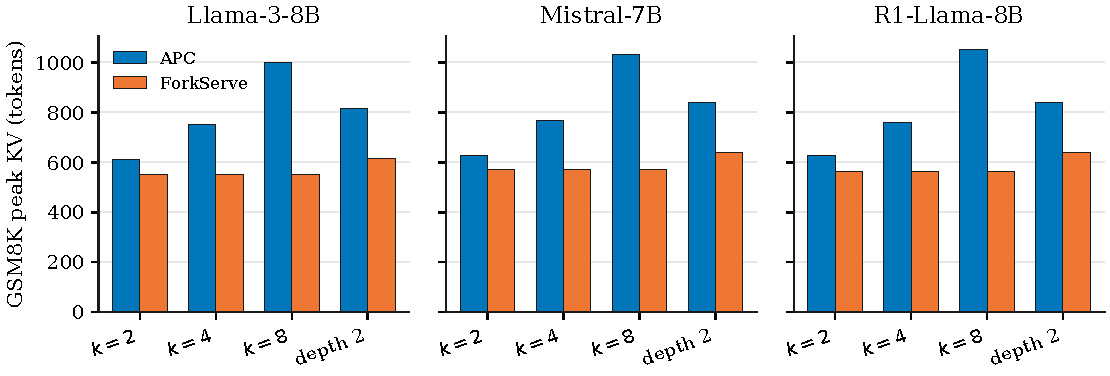
\includegraphics[width=\columnwidth]{fig/branch_peak.pdf}
\caption{\textbf{GSM8K peak KV versus branching} ($n{=}16$, $\mathrm{tp}{=}2$, $D{=}512$).
ForkServe+ matches the ForkServe bar.
The spine peak is invariant in $k$; the APC peak grows with the hashed union, so the ratio falls from $0.89$--$0.90$ to $0.53$--$0.55$.}
\label{fig:eval-branch}
\end{figure}

\paragraph{The ratio falls with $k$.}
\Cref{tab:branch,fig:eval-branch} measures $(L+\ell)/(L+k\ell)$ on the GPU. The spine peak is invariant in $k$ while the APC peak increases, so the ratio moves from $0.89$--$0.90$ at $k{=}2$ to $0.53$--$0.55$ at $k{=}8$ on all three families.
At depth $2$ the ratio is $0.75$--$0.76$.
ForkServe+ leaves the peak unchanged. At $k{=}8$ it rejects $28$ branches and reduces fan-out from $307$ to $179$\,ms on Llama-3-8B, from $349$ to $191$\,ms on Mistral-7B, and from $363$ to $194$\,ms on DeepSeek-R1.
With draft pruning disabled, Llama-3-8B fan-out is $247$\,ms and DeepSeek-R1 fan-out is $271$\,ms.
% The last-line stop is not the decode cut here: the winner already ends inside $D$, so emitted tokens stay near $2500$--$7000$ against APC's $8192$.
A batch of $16$ keeps the ratio at $0.72$--$0.73$ ($2071/2871$ on Llama-3-8B, $2135/2935$ on Mistral-7B, $2093/2893$ on DeepSeek-R1).

\begin{table}[t]
\centering
\caption{Contest forest, $D{=}2048$, $k{=}4$, $\mathrm{tp}{=}2$.
MATH-500 is $n{=}200$; AIME is $n{=}73$.
R1 is DeepSeek-R1; 4B is Qwen3-4B.
Best storage and shortest end-to-end time in green.}
\label{tab:longcot}
\scriptsize
\setlength{\tabcolsep}{2.4pt}
\setlength{\aboverulesep}{0.35pt}
\setlength{\belowrulesep}{0.35pt}
\begin{tabular}{llrrrr}
\rowcolor{tblhead}
\toprule
Model & Method & peak & / APC & acc. & e2e (s) \\
\midrule
 & APC & $1863$ & --- & $0.560$ & $429$ \\
\rowcolor{tblalt}
 & FS & \win{$1391$} & \win{$0.75$} & $0.510$ & $432$ \\
\multirow{-3}{*}{R1 MATH}
 & FS+ & $1599$ & $0.86$ & $0.545$ & \win{$247$} \\
\midrule
 & APC & $2118$ & --- & $0.055$ & $178$ \\
\rowcolor{tblalt}
 & FS & \win{$1646$} & \win{$0.78$} & $0.123$ & $178$ \\
\multirow{-3}{*}{R1 AIME}
 & FS+ & $1662$ & $0.78$ & $0.096$ & \win{$165$} \\
\midrule
 & APC & $1937$ & --- & $0.620$ & $329$ \\
\rowcolor{tblalt}
 & FS & \win{$1770$} & \win{$0.91$} & $0.625$ & $248$ \\
\multirow{-3}{*}{4B MATH}
 & FS+ & \win{$1770$} & \win{$0.91$} & $0.600$ & \win{$236$} \\
\midrule
 & APC & $2150$ & --- & $0.027$ & $136$ \\
\rowcolor{tblalt}
 & FS & \win{$1794$} & \win{$0.83$} & $0.041$ & $136$ \\
\multirow{-3}{*}{4B AIME}
 & FS+ & \win{$1794$} & \win{$0.83$} & $0.041$ & \win{$131$} \\
\bottomrule
\end{tabular}
\end{table}

At $D{=}2048$ the ratio is $0.75$--$0.91$ (\Cref{tab:longcot}).
On MATH-500, ForkServe matches APC ($432$\,s vs.\ $429$\,s on DeepSeek-R1).
ForkServe+ cuts DeepSeek-R1 from $429$\,s to $247$\,s and Qwen3-4B from $329$\,s to $236$\,s; the Qwen3-4B $n{=}32$ slice is $38$\,s versus $53$\,s.
ForkServe+ cuts MATH-500 fan-out from $2406$ to $1284$\,ms on DeepSeek-R1 and from $2787$ to $1014$\,ms on Qwen3-4B, against APC at $1593$ and $1201$\,ms.
Qwen3-4B ForkServe+ scores $120/200$ on MATH-500 (APC $124/200$).

\section{Related Work}
\label{sec:related}

\paragraph{Request-level serving.}
Orca~\cite{orca} introduced iteration-level scheduling; vLLM~\cite{vllm} paged the KV cache and hashes full blocks for APC; SGLang~\cite{sglang} added radix prefix sharing; Sarathi~\cite{sarathi,sarathisplit} chunked prefills; DistServe and Splitwise~\cite{distserve,splitwise} disaggregated prefill from decode.
Prefix caching discovers sharing after tokens exist, and prefill--decode disaggregation transfers every page the prefiller produced.
\eqref{eq:action} uses the hash as $m_i$ and the connector as $\Xfer_i$: both are instances of one residual action.

\paragraph{Program- and SLO-aware scheduling.}
Autellix~\cite{autellix} schedules by program-level attained service; JITServe~\cite{jitserve} allocates just-enough bandwidth under heterogeneous SLOs.
Hermes~\cite{hermes}, ThunderAgent~\cite{thunderagent}, and SAGA~\cite{saga} raise the scheduling unit to the program or workflow.
These systems leave KV unshared across children and leave unissued children unprefilled.

\paragraph{KV retention and overlap.}
InferCept~\cite{infercept}, Continuum~\cite{continuum}, MORI~\cite{mori}, and ConServe~\cite{conserve} keep the \emph{current} context alive or placed.
Sutradhara~\cite{sutradhara} overlaps tool execution with prefill of one linear tool-independent prefix.
SmoothAgent~\cite{smoothagent} lookahead-transforms context; IdleSpec~\cite{idlespec} drafts plans for accuracy, not KV.
Classical speculative decoding~\cite{speculative,medusa,eagledraft} drafts \emph{output} tokens.
ForkKV~\cite{forkkv} copy-on-write splits LoRA residuals.
\eqref{eq:action} likewise aliases the shared prefix, then sets $\Work_i$ and $\Xfer_i$ from the unmatched suffix.

\paragraph{Decoding-time pruning.}
A second line drops a candidate after the model has generated it.
Beam search in Tree-of-Thoughts~\cite{tot} scores a finished step and keeps the top beams.
Early-stopping self-consistency (ESC)~\cite{esc} draws a window of complete samples and skips later samples only once that window agrees.
Speculative Rejection~\cite{specrej} ranks partial generations and halts the lower quantile.
Dynamic Parallel Tree Search (DPTS)~\cite{dpts} generates a fixed mini-step on every active node, then early-stops low-confidence children.
In each method the score is computed from tokens already resident, so the prefill and a decode prefix precede the drop.
\eqref{eq:action} withholds $i{\in}\Lambda$ before that prefill and continues every other low score past $t_0$ only if $s'_i{\ge}\tau$ (\S\ref{sec:eval-prefill}).

\section{Conclusion}
\label{sec:conclusion}

Disaggregated prefill transfers every computed page, and a prefix cache retains aborted residuals until eviction.
\sys replaces both with one action per residual: prefill and transfer equal the suffix absent from the radix index, a repeated loop is omitted, and a score below $\tau$ continues past $t_0$ tokens only when the generated prefix meets $\tau$.
Because the trunk is an alias, that suffix excludes $L$, and abort leaves the spine $b(L+\ell_\star)$.

On Qwen3-8B GSM8K ($n{=}16$, $D{=}512$), $\tau_{\mathrm{pre}}{=}0.15$ ahead of ESC, Speculative Rejection, and DPTS attains $15/16$, $16/16$, $16/16$ at $k{=}4,8,16$, cuts computed prefill by $23\%$ ($5008$ to $3848$ at $k{=}16$), and reduces ESC time from $17.05$\,s to $14.14$\,s at $k{=}16$.
$\tau_{\mathrm{pre}}{=}0.45$ reaches $10.93$\,s at $k{=}16$ with the same $16/16$ and loses two problems at $k{=}4$ and $k{=}8$.
On MATH-500 ($n{=}32$, $D{=}1024$), withholding every score below $\tau$ drops any-finished accuracy from $20/32$ to $13/32$ at $k{=}16$; a $128$-token probe restores $20/32$ and lowers end-to-end time from $104.1$\,s to $72.2$\,s.
The Qwen3-14B spine is $0.72\times$ the median APC peak at matched accuracy ($0.845$ vs.\ $0.844$).
Across six families the ratio stays in $0.72$--$0.75\times$ and falls from $0.89$--$0.90\times$ at $k{=}2$ to $0.53$--$0.55\times$ at $k{=}8$.
At a $2048$-token budget it remains $0.75$--$0.91\times$.

The same action sets the kernel, the connector payload, and the KV that remains.
Occupancy depends on $k$ and residual length, not on tensor-parallel width.
As fan-out, depth, and context grow against a fixed pool, each new branch aliases the trunk and abort returns only its residual.


{\small
\begin{thebibliography}{10}

\bibitem{infercept}
Reyna Abhyankar, Zijian He, Vikranth Srivatsa, Hao Zhang, and Yiying Zhang.
\newblock {InferCept: Efficient Intercept Support for Augmented Large Language
  Model Inference}.
\newblock In {\em ICML}, 2024.

\bibitem{sarathi}
Amey Agrawal, Nitin Kedia, Ashish Panwar, Jayashree Mohan, Nipun Kwatra,
  Bhargav Gulavani, Alexey Tumanov, and Ramachandran Ramjee.
\newblock {Taming Throughput-Latency Tradeoff in {LLM} Inference with
  {Sarathi-Serve}}.
\newblock In {\em OSDI}, 2024.

\bibitem{sarathisplit}
Amey Agrawal, Ashish Panwar, Jayashree Mohan, Nipun Kwatra, Bhargav~S.
  Gulavani, and Ramachandran Ramjee.
\newblock {{SARATHI}: Efficient {LLM} Inference by Piggybacking Decodes with
  Chunked Prefills}.
\newblock In {\em arXiv:2308.16369}, 2023.

\bibitem{claude_code}
{Anthropic}.
\newblock {Claude Code}.
\newblock {\em https://docs.anthropic.com/en/docs/claude-code}, 2025.

\bibitem{spork}
Huajun Bai, Weiwei Lv, Huichuan Zheng, Youyou Lu, and Jiwu Shu.
\newblock {SPORK: Self-Speculative Forking to Accelerate Agentic {LLM}
  Inference}.
\newblock {\em arXiv:2607.03333}, 2026.

\bibitem{sutradhara}
Anish Biswas, Kanishk Goel, Srivarshinee S, Jayashree Mohan, Alind Khare,
  Anjaly Parayil, Ramachandran Ramjee, and Chetan Bansal.
\newblock {Sutradhara: An Intelligent Orchestrator-Engine Co-design for
  Tool-based Agentic Inference}.
\newblock {\em arXiv:2601.12967}, 2026.

\bibitem{medusa}
Tianle Cai, Yuhong Li, Zhengyang Geng, Hongwu Peng, Jason~D. Lee, Deming Chen,
  and Tri Dao.
\newblock {Medusa: Simple {LLM} Inference Acceleration Framework with Multiple
  Decoding Heads}.
\newblock In {\em ICML}, 2024.

\bibitem{murakkab}
Gohar~Irfan Chaudhry, Esha Choukse, Haoran Qiu, {\'I}{\~n}igo Goiri, Rodrigo
  Fonseca, Adam Belay, and Ricardo Bianchini.
\newblock {Murakkab: Resource-Efficient Agentic Workflow Orchestration in Cloud
  Platforms}.
\newblock In {\em OSDI}, 2026.

\bibitem{idlespec}
Daewon Choi, Kyunghyun Park, Woomin Song, Saket Dingliwal, Sai~Muralidhar
  Jayanthi, Jinwoo Shin, and Aram Galstyan.
\newblock {IdleSpec: Exploiting Idle Time via Speculative Planning for {LLM}
  Agents}.
\newblock {\em arXiv:2605.22154}, 2026.

\bibitem{contextrot}
{Chroma Research}.
\newblock {Context Rot: How Increasing Input Tokens Impacts {LLM} Performance}.
\newblock {\em https://research.trychroma.com/context-rot}, 2025.

\bibitem{conserve}
Jianru Ding, Ryien Hosseini, Pouya~Mahdi Gholami, Mingyuan Xiang, and Henry
  Hoffmann.
\newblock {Observation, Not Prediction: Conversation-Level Disaggregated
  Scheduling for Agentic Serving}.
\newblock {\em arXiv:2606.01839}, 2026.

\bibitem{pie}
In~Gim, Zhiyao Ma, Seung-seob Lee, and Lin Zhong.
\newblock {Pie: A Programmable Serving System for Emerging {LLM} Applications}.
\newblock In {\em SOSP}, 2025.

\bibitem{saga}
Dongxin Guo, Jikun Wu, and Siu-Ming Yiu.
\newblock {SAGA: Workflow-Atomic Scheduling for {AI} Agent Inference on {GPU}
  Clusters}.
\newblock In {\em HPDC}, 2026.

\bibitem{metagpt}
Sirui Hong, Mingchen Zhuge, Jonathan Chen, Xiawu Zheng, Yuheng Cheng, Jinlin
  Wang, Ceyao Zhang, Zili Wang, Steven Ka~Shing Yau, Zijuan Lin, Liyang Zhou,
  Chenyu Ran, Lingfeng Xiao, Chenglin Wu, and J{\"u}rgen Schmidhuber.
\newblock {MetaGPT: Meta Programming for A Multi-Agent Collaborative
  Framework}.
\newblock {\em ICLR}, 2024.

\bibitem{swebench}
Carlos~E. Jimenez, John Yang, Alexander Wettig, Shunyu Yao, Kexin Pei, Ofir
  Press, and Karthik Narasimhan.
\newblock {SWE-bench: Can Language Models Resolve Real-World {GitHub} Issues?}
\newblock {\em ICLR}, 2024.

\bibitem{thunderagent}
Hao Kang, Ziyang Li, Xinyu Yang, Weili Xu, Yinfang Chen, Junxiong Wang, Beidi
  Chen, Tushar Krishna, Chenfeng Xu, and Simran Arora.
\newblock {ThunderAgent: A Simple, Fast and Program-Aware Agentic Inference
  System}.
\newblock {\em arXiv:2602.13692}, 2026.

\bibitem{vllm}
Woosuk Kwon, Zhuohan Li, Siyuan Zhuang, Ying Sheng, Lianmin Zheng, Cody~Hao Yu,
  Joseph Gonzalez, Hao Zhang, and Ion Stoica.
\newblock {Efficient Memory Management for Large Language Model Serving with
  {PagedAttention}}.
\newblock In {\em SOSP}, 2023.

\bibitem{speculative}
Yaniv Leviathan, Matan Kalman, and Yossi Matias.
\newblock {Fast Inference from Transformers via Speculative Decoding}.
\newblock {\em ICML}, 2023.

\bibitem{dpts}
Yifu Ding, Wentao Jiang, Shunyu Liu, Yongcheng Jing, Jinyang Guo, Yingjie
  Wang, Jing Zhang, Zengmao Wang, Ziwei Liu, Bo Du, Xianglong Liu, and
  Dacheng Tao.
\newblock {Dynamic Parallel Tree Search for Efficient {LLM} Reasoning}.
\newblock In {\em ACL}, 2025.

\bibitem{continuum}
Hanchen Li, Runyuan He, Qiuyang Mang, Qizheng Zhang, Huanzhi Mao, Xiaokun Chen,
  Hangrui Zhou, Alvin Cheung, Joseph Gonzalez, and Ion Stoica.
\newblock {Continuum: Efficient and Robust Multi-Turn {LLM} Agent Scheduling
  with {KV} Cache Time-to-Live}.
\newblock {\em arXiv:2511.02230}, 2025.

\bibitem{esc}
Yiwei Li, Peiwen Yuan, Shaoxiong Feng, Boyuan Pan, Xinglin Wang, Bin Sun,
  Heda Wang, and Kan Li.
\newblock {Escape Sky-High Cost: Early-Stopping Self-Consistency for
  Multi-Step Reasoning}.
\newblock In {\em ICLR}, 2024.

\bibitem{eagledraft}
Yuhong Li, Fangyun Wei, Chao Zhang, and Hongyang Zhang.
\newblock {EAGLE: Speculative Sampling Requires Rethinking Feature
  Uncertainty}.
\newblock In {\em ICML}, 2024.

\bibitem{parrot}
Chaofan Lin, Zhenhua Han, Chengruidong Zhang, Yuqing Yang, Fan Yang, Chen Chen,
  and Lili Huang.
\newblock {Parrot: Efficient Serving of {LLM}-based Applications with Semantic
  Variable}.
\newblock In {\em OSDI}, 2024.

\bibitem{hermes}
Yifei Liu, Zuo Gan, Zhenghao Gan, Weiye Wang, Chen Chen, Yizhou Shan, Xusheng
  Chen, Zhenhua Han, Yifei Zhu, Shixuan Sun, and Minyi Guo.
\newblock {Efficient Serving of {LLM} Applications with Probabilistic Demand
  Modeling}.
\newblock {\em arXiv:2506.14851}, 2025.

\bibitem{autellix}
Michael Luo, Xiaoxiang Shi, Colin Cai, Tianjun Zhang, Justin Wong, Yichuan
  Wang, Chi Wang, Yanping Huang, Zhifeng Chen, Joseph~E. Gonzalez, and Ion
  Stoica.
\newblock {Autellix: An Efficient Serving Engine for {LLM} Agents as General
  Programs}.
\newblock {\em arXiv:2502.13965}, 2025.

\bibitem{hive}
Zizhang Luo, Yuhao Luo, Youwei Xiao, Yansong Xu, Runlin Guo, and Yun Liang.
\newblock {Hive: A Multi-Agent Infrastructure for Algorithm- and Task-Level
  Scaling}.
\newblock {\em arXiv:2604.17353}, 2026.

\bibitem{gaia}
Gr{\'e}goire Mialon, Cl{\'e}mentine Fourrier, Craig Swift, Thomas Wolf, Yann
  LeCun, and Thomas Scialom.
\newblock {GAIA: a Benchmark for General {AI} Assistants}.
\newblock {\em arXiv:2311.12983}, 2023.

\bibitem{astraea}
Hongqiu Ni, Jiabao Zhang, Guopeng Li, Zilong Wang, Ruiqi Wu, Chi Zhang, and
  Haisheng Tan.
\newblock {Astraea: A State-Aware Scheduling Engine for {LLM}-Powered Agents}.
\newblock {\em arXiv:2512.14142}, 2025.

\bibitem{memgpt}
Charles Packer, Vivian Fang, Shishir~G. Patil, Kevin Lin, Sarah Wooders, and
  Joseph~E. Gonzalez.
\newblock {MemGPT: Towards {LLMs} as Operating Systems}.
\newblock {\em arXiv:2310.08560}, 2023.

\bibitem{smoothagent}
Zaifeng Pan, Qianxu Wang, Zhengding Hu, Chang Chen, Yue Guan, Yanbo Zhou,
  Steven Swanson, and Yufei Ding.
\newblock {SmoothAgent: Efficient Long-Horizon {LLM}-Based Agent Serving with
  Lookahead Context Engineering}.
\newblock {\em arXiv:2607.00151}, 2026.

\bibitem{specrej}
Hanshi Sun, Momin Haider, Ruiqi Zhang, Huitao Yang, Jiahao Qiu, Ming Yin,
  Mengdi Wang, Peter Bartlett, and Andrea Zanette.
\newblock {Fast Best-of-{N} Decoding via Speculative Rejection}.
\newblock In {\em NeurIPS}, 2024.

\bibitem{splitwise}
Pratyush Patel, Esha Choukse, Chaojie Zhang, Aashaka Shah, {\'I}{\~n}igo Goiri,
  Saeed Maleki, and Ricardo Bianchini.
\newblock {Splitwise: Efficient Generative {LLM} Inference Using Phase
  Splitting}.
\newblock In {\em ISCA}, 2024.

\bibitem{gorilla}
Shishir~G. Patil, Tianjun Zhang, Xin Wang, and Joseph~E. Gonzalez.
\newblock {Gorilla: Large Language Model Connected with Massive {APIs}}.
\newblock {\em NeurIPS}, 2024.

\bibitem{osfork}
Dennis~M. Ritchie and Ken Thompson.
\newblock {The UNIX Time-Sharing System}.
\newblock {\em CACM}, 17(7), 1974.

\bibitem{toolformer}
Timo Schick, Jane Dwivedi-Yu, Roberto Dess{\`i}, Roberta Raileanu, Maria
  Lomeli, Eric Hambro, Luke Zettlemoyer, Nicola Cancedda, and Thomas Scialom.
\newblock {Toolformer: Language Models Can Teach Themselves to Use Tools}.
\newblock {\em NeurIPS}, 2023.

\bibitem{ayo}
Xin Tan, Yimin Jiang, Yitao Yang, and Hong Xu.
\newblock {Towards End-to-End Optimization of {LLM}-based Applications with
  {Ayo}}.
\newblock In {\em ASPLOS}, 2025.

\bibitem{tanenbaumos}
Andrew~S. Tanenbaum and Herbert Bos.
\newblock {\em {Modern Operating Systems}}.
\newblock Pearson, 4 edition, 2015.

\bibitem{forkkv}
Shao Wang, Rui Ren, and Lin Gui.
\newblock {ForkKV: Scaling Multi-{LoRA} Agent Serving via Copy-on-Write
  Disaggregated {KV} Cache}.
\newblock {\em arXiv:2604.06370}, 2026.

\bibitem{openhands}
Xingyao Wang, Boxuan Li, Yufan Song, Frank~F. Xu, Xiangru Tang, Mingchen Zhuge,
  Jiayi Pan, Yueqi Song, Bowen Li, Jaskirat Singh, Hoang~H. Tran, Fuqiang Li,
  Ren Ma, Mingzhang Zheng, Bill Qian, Yanjun Shao, Niklas Muennighoff, Yizhe
  Zhang, Binyuan Hui, Junyang Lin, Robert Brennan, Hao Peng, Heng Ji, and
  Graham Neubig.
\newblock {OpenHands: An Open Platform for {AI} Software Developers as
  Generalist Agents}.
\newblock {\em ICLR}, 2025.

\bibitem{selfconsistency}
Xuezhi Wang, Jason Wei, Dale Schuurmans, Quoc Le, Ed~Chi, Sharan Narang,
  Aakanksha Chowdhery, and Denny Zhou.
\newblock {Self-Consistency Improves Chain of Thought Reasoning in Language
  Models}.
\newblock {\em ICLR}, 2023.

\bibitem{augserve}
Ying Wang, Zhen Jin, Zhenqian Chen, Jiexiong Xu, Wenhai Lin, Yiquan Chen, and
  Wenzhi Chen.
\newblock {AugServe: Adaptive Request Scheduling for Augmented Large Language
  Model Inference Serving}.
\newblock In {\em ICML}, 2026.

\bibitem{autogen}
Qingyun Wu, Gagan Bansal, Jieyu Zhang, Yiran Wu, Beibin Li, Erkang Zhu,
  Li~Jiang, Xiaoyun Zhang, Shaokun Zhang, Jiale Liu, Ahmed~Hassan Awadallah,
  Ryen~W. White, Doug Burger, and Chi Wang.
\newblock {AutoGen: Enabling Next-Gen {LLM} Applications via Multi-Agent
  Conversation}.
\newblock {\em arXiv:2308.08155}, 2023.

\bibitem{mori}
Tian Xia, Hanchen Li, Zhifei Li, Xiaokun Chen, Hao Kang, Yifan Qiao, Yi~Xu, and
  Ion Stoica.
\newblock {Idleness is Relative: Exploiting Tool-Call Idle Windows for
  Offloading in Agentic Systems with {MORI}}.
\newblock {\em arXiv:2606.00866}, 2026.

\bibitem{sweagent}
John Yang, Carlos~E. Jimenez, Alexander Wettig, Kilian Lieret, Shunyu Yao,
  Karthik Narasimhan, and Ofir Press.
\newblock {SWE-agent: Agent-Computer Interfaces Enable Automated Software
  Engineering}.
\newblock {\em NeurIPS}, 2024.

\bibitem{tot}
Shunyu Yao, Dian Yu, Jeffrey Zhao, Izhak Shafran, Thomas~L. Griffiths, Yuan
  Cao, and Karthik Narasimhan.
\newblock {Tree of Thoughts: Deliberate Problem Solving with Large Language
  Models}.
\newblock {\em NeurIPS}, 2023.

\bibitem{react}
Shunyu Yao, Jeffrey Zhao, Dian Yu, Nan Du, Izhak Shafran, Karthik Narasimhan,
  and Yuan Cao.
\newblock {ReAct: Synergizing Reasoning and Acting in Language Models}.
\newblock {\em ICLR}, 2023.

\bibitem{orca}
Gyeong-In Yu, Joo~Seong Jeong, Geon-Woo Kim, Soojeong Kim, and Byung-Gon Chun.
\newblock {Orca: A Distributed Serving System for {Transformer-Based}
  Generative Models}.
\newblock In {\em OSDI}, 2022.

\bibitem{pythia}
Shan Yu, Junyi Shu, Yuanjiang Ni, Kun Qian, Xue Li, Yang Wang, Jinyuan Zhang,
  Ziyi Xu, Shuo Yang, Lingjun Zhu, Ennan Zhai, Qingda Lu, Jiarong Xing, Youyou
  Lu, Xin Jin, Xuanzhe Liu, and Harry Xu.
\newblock {Pythia: Exploiting Workflow Predictability for Efficient
  Agent-Native {LLM} Serving}.
\newblock {\em arXiv:2604.25899}, 2026.

\bibitem{kairospower}
Yichao Yuan, Mosharaf Chowdhury, and Nishil Talati.
\newblock {KAIROS: Stateful, Context-Aware Power-Efficient Agentic Inference
  Serving}.
\newblock {\em arXiv:2604.16682}, 2026.

\bibitem{compoundai}
Matei Zaharia, Omar Khattab, Lingjiao Chen, Jared McCauley, et~al.
\newblock {The Shift from Models to Compound {AI} Systems}.
\newblock {\em Berkeley AI Research Blog}, 2024.

\bibitem{mctsllm}
Di~Zhang et~al.
\newblock {Accessing GPT-4 Level Mathematical Olympiad Solutions via Monte
  Carlo Tree Self-refine}.
\newblock {\em arXiv:2312.11324}, 2023.

\bibitem{jitserve}
Wei Zhang, Zhiyu Wu, Yi~Mu, Rui Ning, Banruo Liu, Nikhil Sarda, Myungjin Lee,
  and Fan Lai.
\newblock {JITServe: {SLO}-aware {LLM} Serving with Imprecise Request
  Information}.
\newblock In {\em NSDI}, 2026.

\bibitem{sglang}
Lianmin Zheng, Liangsheng Yin, Zhiqiang Xie, Chuyue Sun, Jeff Huang, Cody~Hao
  Yu, Shiyi Cao, Christos Kozyrakis, Ion Stoica, Joseph~E. Gonzalez, Clark
  Barrett, and Ying Sheng.
\newblock {SGLang: Efficient Execution of Structured Language Model Programs}.
\newblock In {\em NeurIPS}, 2024.

\bibitem{distserve}
Yinmin Zhong, Shengyu Liu, Junda Chen, Jianbo Hu, Yibo Zhu, Xuanzhe Liu, Xin
  Jin, and Hao Zhang.
\newblock {DistServe: Disaggregating Prefill and Decoding for Goodput-optimized
  Large Language Model Serving}.
\newblock In {\em OSDI}, 2024.

\bibitem{webarena}
Shuyan Zhou, Frank~F. Xu, Hao Zhu, Xuhui Zhou, Robert Lo, Abhijit Sridhar,
  Xianyi Cheng, Tianyue Ou, Yonatan Bisk, Daniel Fried, Uri Alon, and Graham
  Neubig.
\newblock {WebArena: A Realistic Web Environment for Building Autonomous
  Agents}.
\newblock {\em ICLR}, 2024.

\end{thebibliography}

}

\end{document}
